\documentclass[a4paper,10pt,english]{article}
%\documentclass[12pt,preprint]{aastex}
\usepackage[utf8]{inputenc}
\usepackage[margin=0.5in]{geometry} % narrow margins
\usepackage{amsfonts}
\usepackage{graphicx}
\usepackage{float}
\usepackage{cite}
\usepackage{amsmath}
\usepackage{epsfig,floatflt}
\usepackage{hyperref}
\usepackage{listings}
\usepackage[table,xcdraw]{xcolor}
\usepackage{booktabs}
\usepackage{subfig}
\usepackage{algpseudocode}
\usepackage{algorithm}
%\usepackage{amsmath,graphicx,varioref,verbatim,amsfonts,geometry,amssymb,dsfont,blindtext}
\hypersetup{colorlinks=true}
\usepackage{xcolor}
\usepackage{hhline}
\usepackage[export]{adjustbox}
\definecolor{LightGray}{gray}{0.95}
\definecolor{dkgreen}{rgb}{0,0.6,0}
\definecolor{gray}{rgb}{0.5,0.5,0.5}
\definecolor{mauve}{rgb}{0.58,0,0.82}
\definecolor{mygray}{rgb}{0.9,0.9,0.9}
\definecolor{LightGray}{gray}{0.95}
\lstset{frame=tb,
	language=Python,
	aboveskip=3mm,
	belowskip=3mm,
	showstringspaces=false,
	columns=flexible,
	basicstyle={\small\ttfamily},
	numbers=none,
	numberstyle=\tiny\color{gray},
	keywordstyle=\color{blue},
	commentstyle=\color{dkgreen},
	stringstyle=\color{mauve},
	backgroundcolor=\color{mygray},
	breaklines=true,
	postbreak=\mbox{\textcolor{red}{$\hookrightarrow$}\space}
	%breakatwhitespace=true,
	%tabsize=3
}

%\usepackage[english]{babel}
%\usepackage{fancyhdr}
%\usepackage{lastpage}
%
%\pagestyle{fancy}
%\fancyhf{}
%
%\rfoot{Page \thepage \hspace{1pt} of \pageref{LastPage}}
\pagenumbering{arabic}

\begin{document}
\title{FYS-STK4155 Project 1}
\author{Bendik Steinsvåg Dalen \& Gabriel Sigurd Cabrera}
%\maketitle

\twocolumn[
\maketitle
\begin{abstract}
	dtcfvgbjhkgvfcdxszeasxrdtgyubhnijhugfvcdfguhij ftufykubhk nj jkdsi jkjk dsjknslj fd,nøj ka n,sdf jknm bnjdsajk nmnj mbfdjksa ,nfdsa mn n,asdf\\\\
\end{abstract}
]


%\begin{@twocolumnfalse}
%%	\maketitle
%	\begin{abstract}
%		dtcfvgbjhkgvfcdxszeasxrdtgyubhnijhugfvcdfguhij ftufykubhk nj jkdsi jkjk dsjknslj fd,nøj ka n,sdf jknm bnjdsajk nmnj mbfdjksa ,nfdsa mn n,asdf
%	\end{abstract}
%\end{@twocolumnfalse}

\section{Introduction}
\label{sec:introduction}

The purpose of this report is to analyze the performance of several regression methods – Ordinary Least Squares (OLS), Ridge Regression, and LASSO\footnote{Short for \textit{least absolute shrinkage and selection operator}.} Regression.  In addition to implementing these regression methods, we will be validating (and cross-validating) our results by calculating the \textit{mean squared error}, \textit{bias}, and \textit{variance}, giving us an understanding of how these models' predictive capabilities vary as functions of complexity.

Once we have a clear picture of how these regression models behave, we hope to determine which model best fits our input data.  This will require analyzing our validation data and determining what complexity and hyperparameter minimizes our total error.

%Things we need to write about:
%
%Background on regression analysis and resampling methods.
%Mention:
%	OLS
%	Ridge
%	LASSO
%	k-fold cross-validation
%	Bias-Variance trade of?
%
%We will first study how they preform for the two dimensional Franke-function. (A bit about the Franke-function, maybe a tldr for the method).
%
%We will then implement them for some real terrain data for Møsvatn Austfjell in Norway. mm. (biggest lake in Norway ) %\cite{https://no.wikipedia.org/wiki/Møsvatn}


%Discuss background, physical importance and possibly some history of
%the problem that is being studied in this paper.




\section{Data}
\label{sec:data}

In this report, we will be working with two separate datasets.

\subsection{The Franke Function}

The first dataset will be given by the \textit{Franke function}, which is defined as follows:

\begin{align*}
f(x,y) &= \frac{3}{4} \exp \left( -\frac{(9x-2)^2}{4} -\frac{(9y-2)^2}{4} \right) \\ &+ \frac{3}{4} \exp \left( -\frac{9x+1}{49} -\frac{9y+1}{10} \right) \\ &+ \frac{1}{2} \exp \left( -\frac{(9x-7)^2}{4} -\frac{(9y-3)^2}{4} \right) \\ &- \frac{1}{5} \exp \left( -(9x-4)^2 - (9y-7)^2 \right)
\end{align*}

We will be solving the Franke function for 100 $x$-values and 100 $y$-values in the range $[0,1]$, leaving us with a grid containing a total of 10000 $xy$ coordinate pairs.  This leaves us with the values plotted in Figure \ref{fig_Franke}.

\begin{figure}[H]
	\centering
	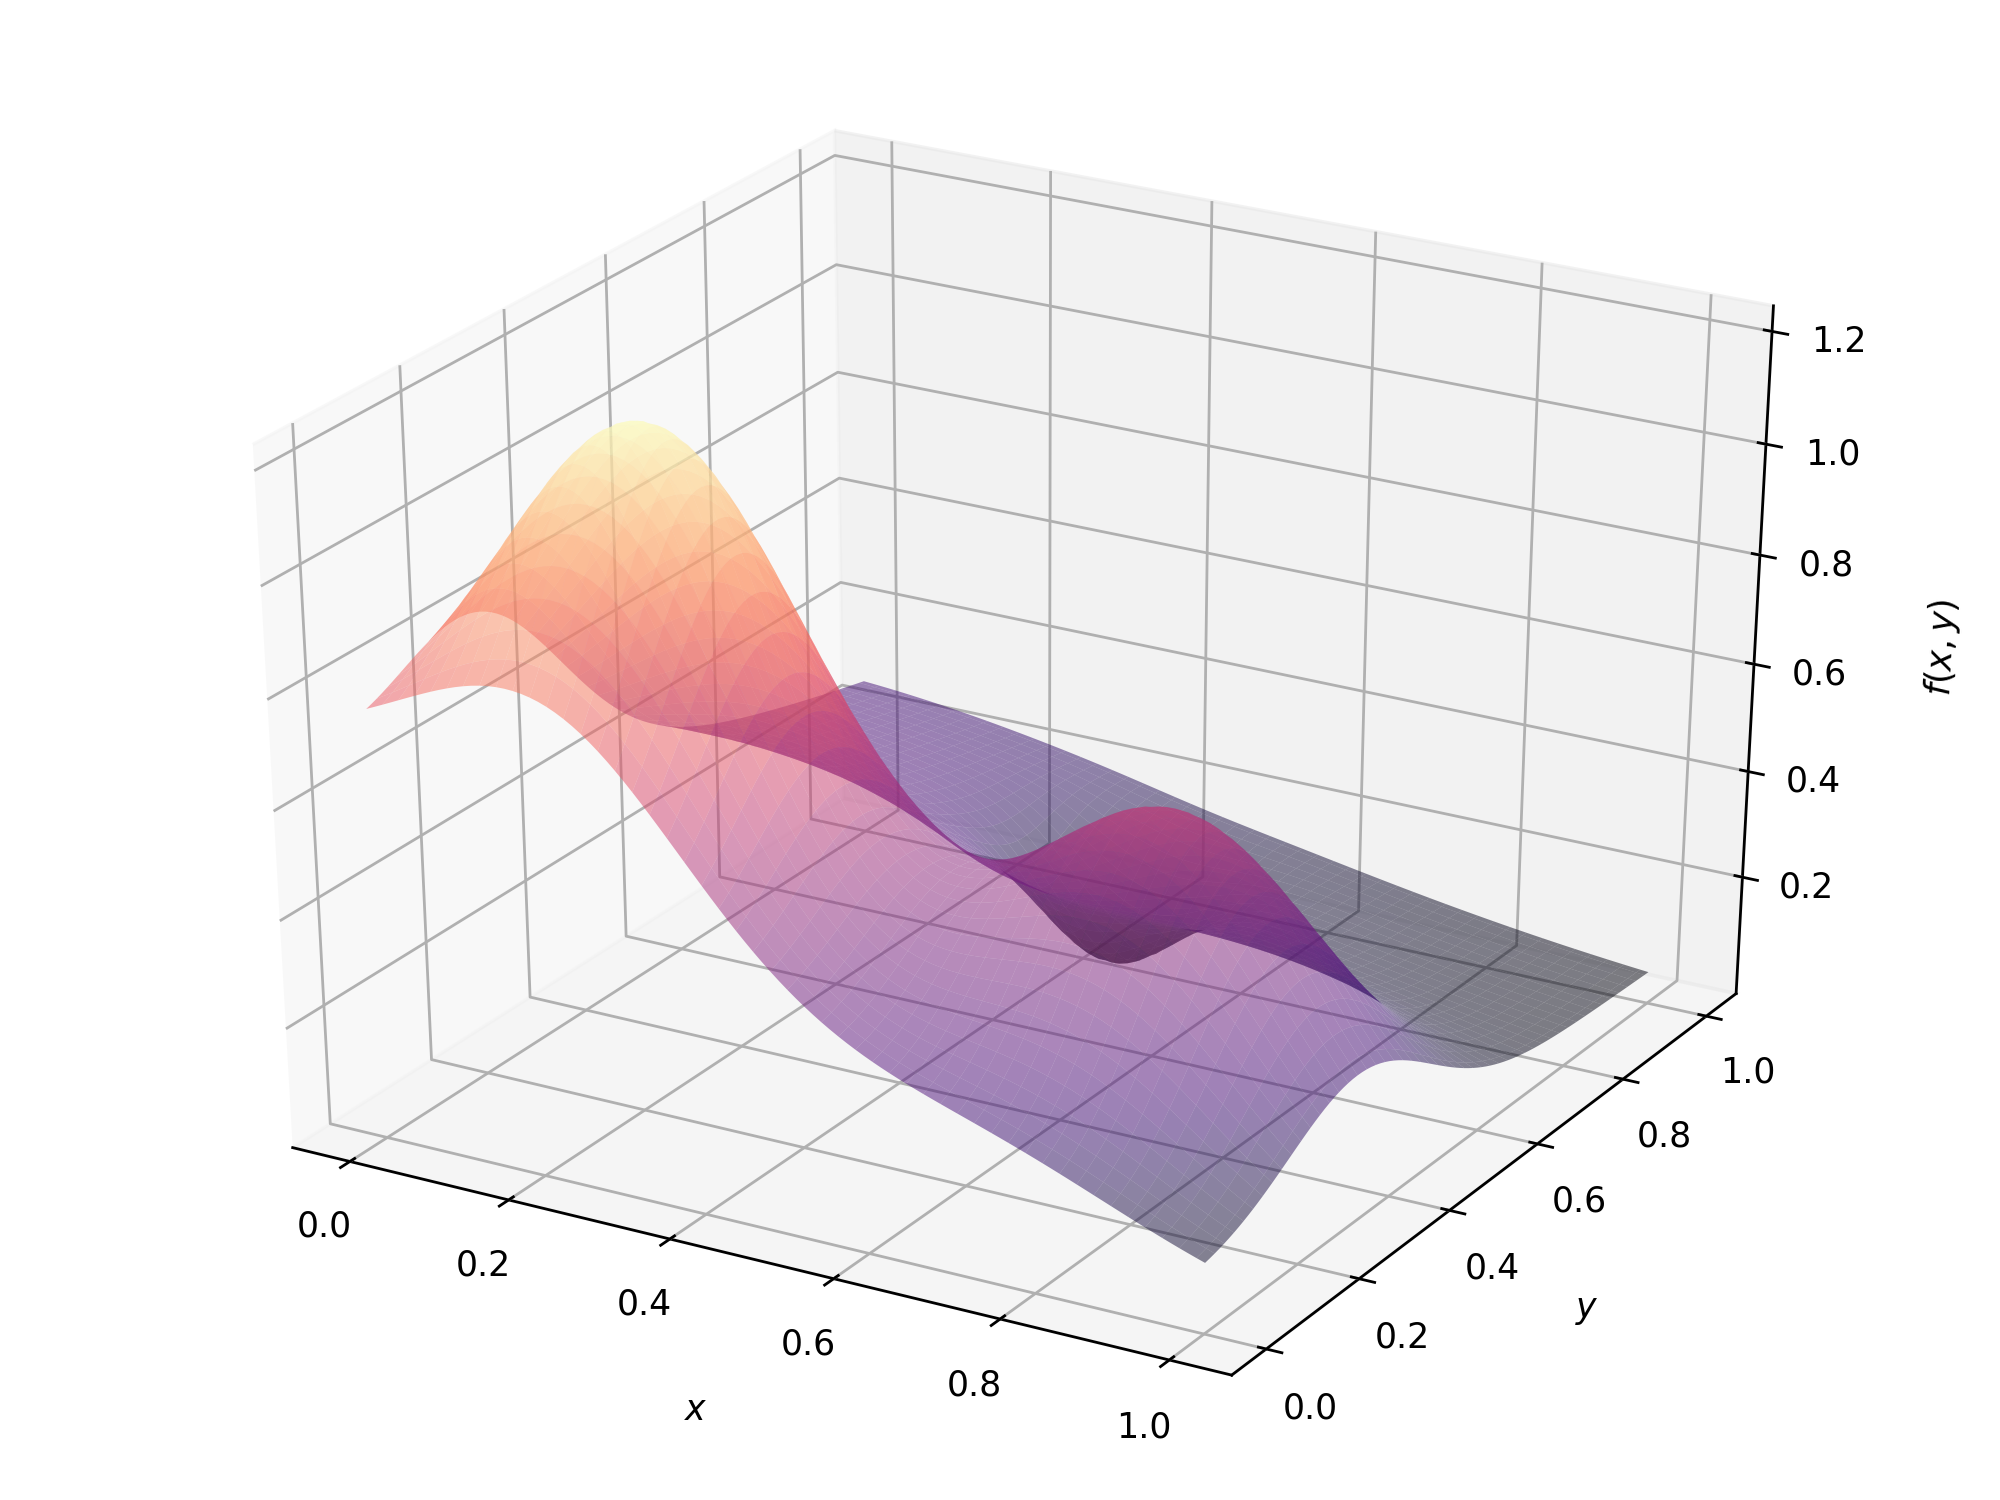
\includegraphics[width = 0.5\textwidth, center]{Franke.png}
	\caption{The \textit{Franke function} for $x$ and $y$ values ranging from zero to one. \label{fig_Franke}}
\end{figure}


In addition, we will also be adding \textit{Gaussian noise} to each value $f(x,y)$, such that we are left with values as seen in Figure \ref{fig_Franke_noise}.

\begin{figure}[H]
	\centering
	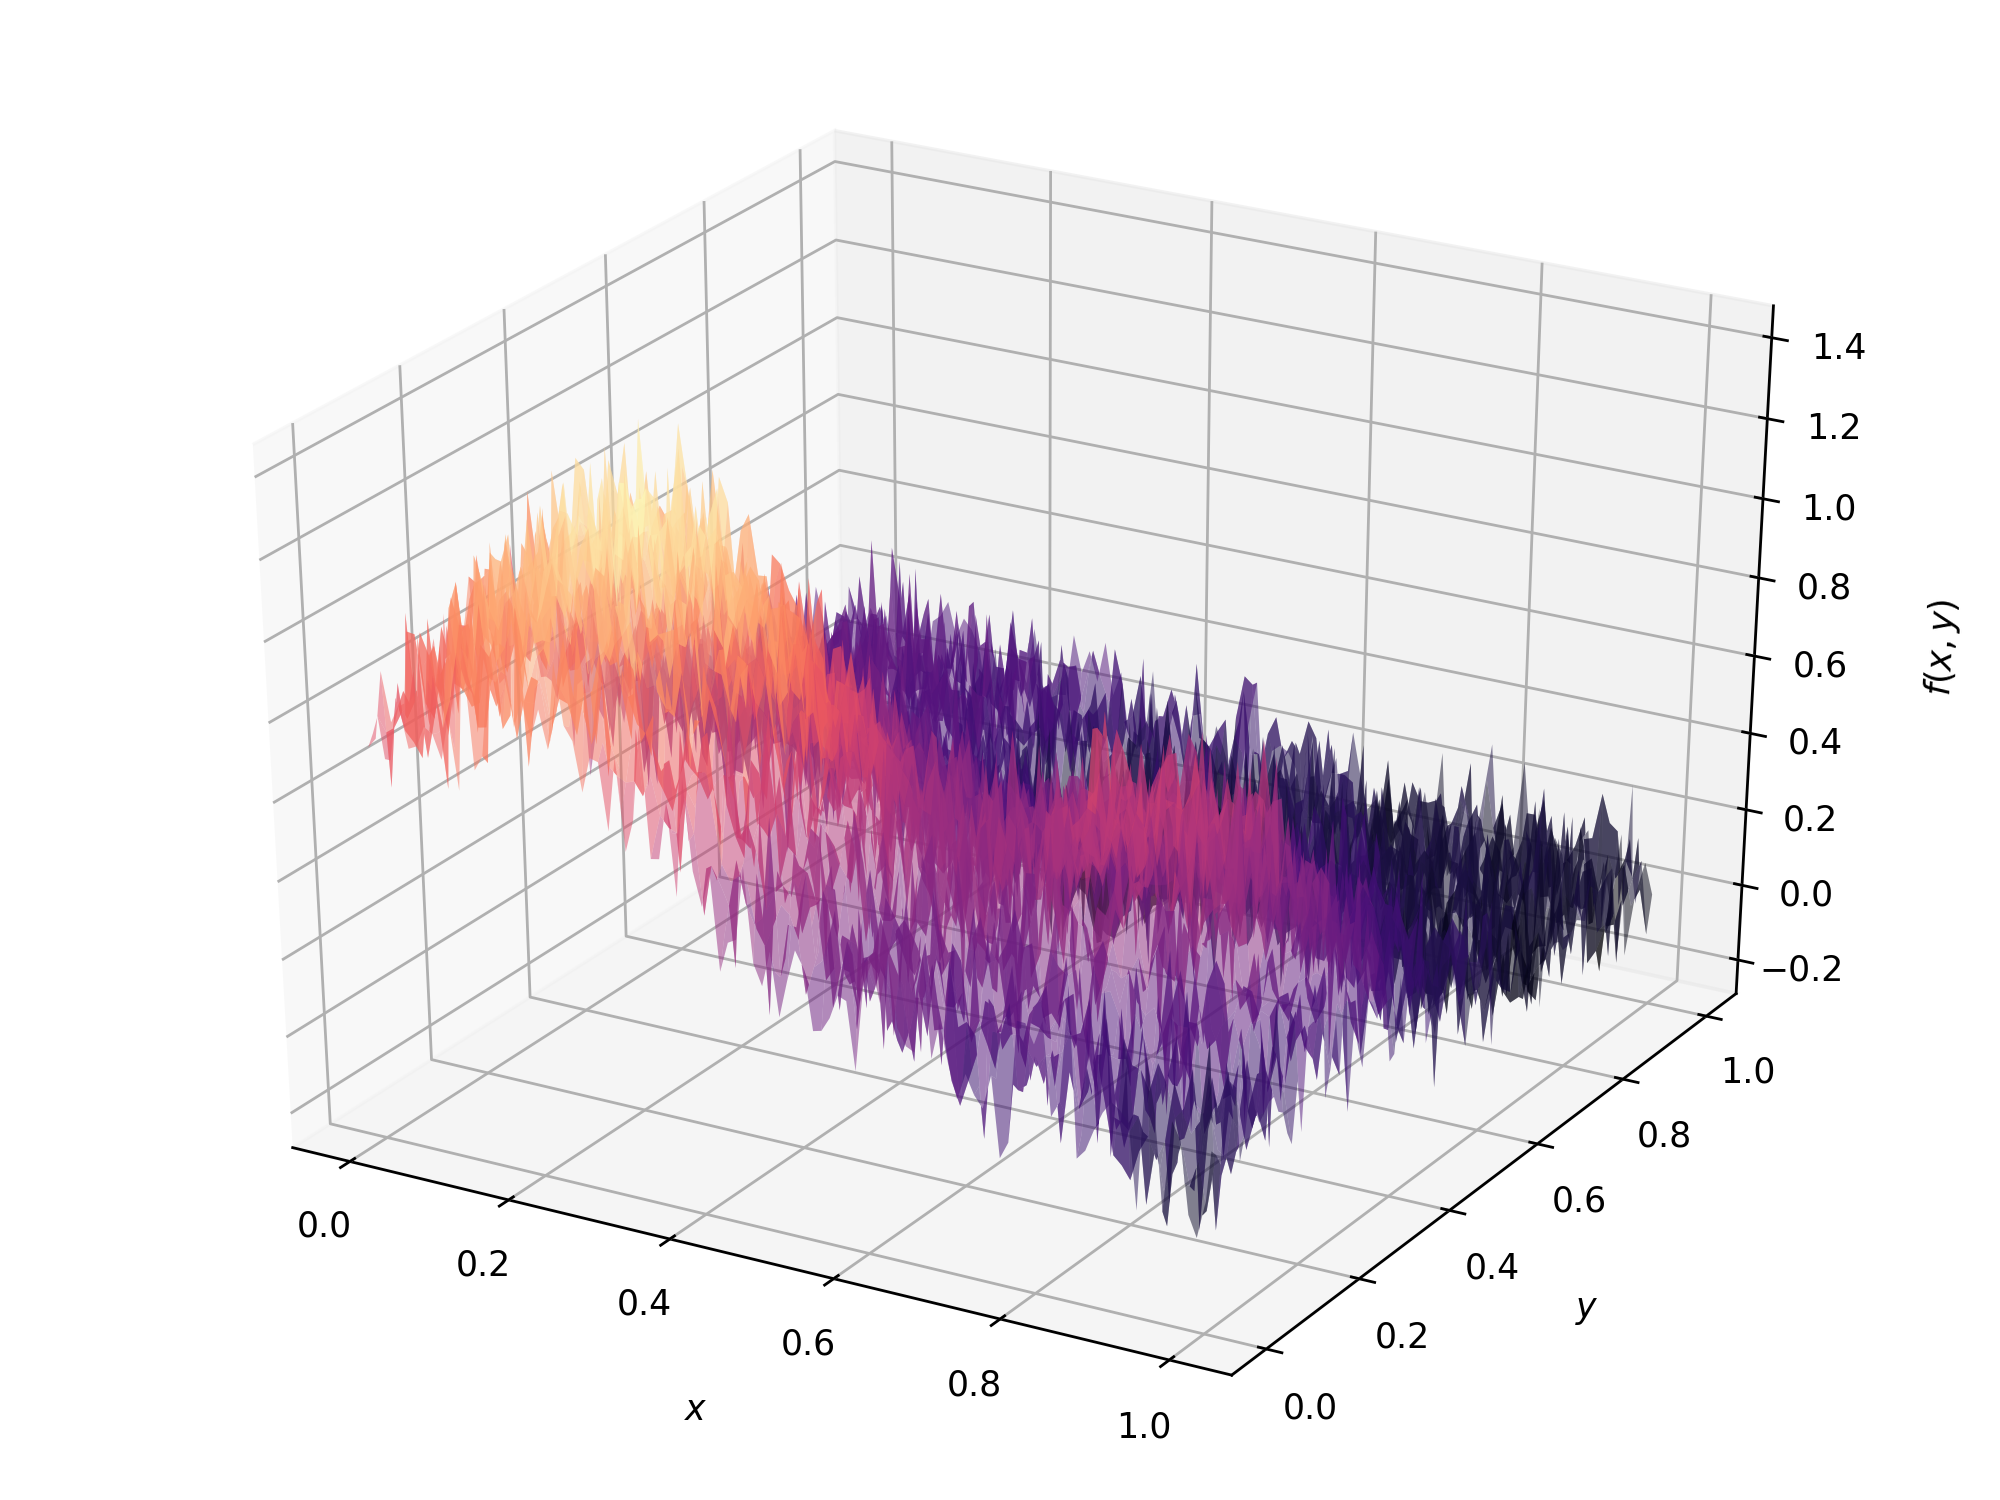
\includegraphics[width = 0.5\textwidth, center]{Franke_noise.png}
	\caption{The \textit{Franke function} for $x$ and $y$ values ranging from zero to one, with a Gaussian noise $N(0,0.01)$\label{fig_Franke_noise}}
\end{figure}

\subsection{Møsvatn Austfjell}

For our second dataset, we will be using real data taken from the \textit{U.S. Geological Survey} \cite{earthexplorer} official website \url{https://earthexplorer.usgs.gov/}.  More specifically, we will be using a \texttt{.tif} file containing altitude data for a rectangular region of Møsvatn Austfjell shown in Figure \ref{fig_austfjell}.

\begin{figure}[H]
	\centering
	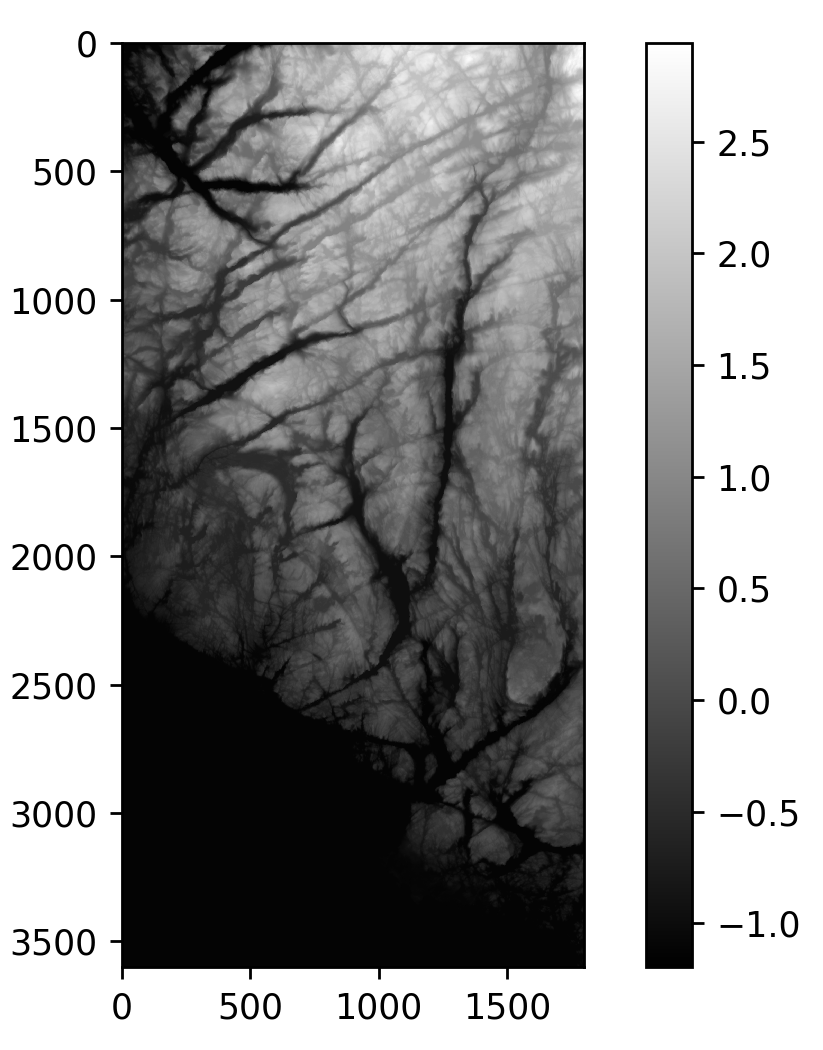
\includegraphics[width = 0.4\textwidth, center]{real_data.png}
	\caption{Altitude data from Møsvatn Austfjell, from the USGS website \cite{earthexplorer}.\label{fig_austfjell}}
\end{figure}	



\section{Method}
\label{sec:method}

\subsection{Generalization of Multidimensional Polynomials}

If we wish to construct a $p$-dimensional polynomial of degree $d$, we need to know what terms need to be included to give us a completely generalized polynomial.  For a 1-D polynomial of second degree, we would have three terms:

\begin{equation*}
f(x) = \beta_1 + \beta_2 x + \beta_3 x^2
\end{equation*}

Where $\beta$ is a vector containing each coefficient.	For a 2-D polynomial of second degree, we would have 6 terms:

\begin{equation*}
f(x,y) = \beta_1 + \beta_2 x + \beta_3 y + \beta_4 xy + \beta_5 x^2 + \beta_6 y^2
\end{equation*}

And for a 3-D polynomial of second degree, we would have 10 terms:

\begin{align*}
f(x,y,z) &= \beta_1 + \beta_2 x + \beta_3 y + \beta_4 z + \beta_5 xy \\ &+ \beta_6 xz + \beta_7 yz + \beta_8 x^2 + \beta_9 y^2 + \beta_{10} z^2
\end{align*}

There are many possible combinations of $p$ and $d$, and the number of terms blows up significantly as these values increase.  We can, however, create a general expression \cite{2482654} for any $p$ and $d$ using summation notation:

\begin{equation}
\label{eq_method_0}
f(\mathbf{x}) = \sum_{\sum_{j = 1}^d i_j \leq p} \left( \beta_{i_1, i_2, \cdots, i_d} \prod_{k = 1}^d x_k^{i_k} \right)
\end{equation}

Alternatively, a simple \texttt{python} script can be used to find all the terms' exponents by calculating all permutations of the natural numbers from zero to $d$ in sets of length $p$, then removing all results whose sum is greater than $d$.

\begin{lstlisting}[showstringspaces=false,language=Python,firstnumber = 1]
powers = np.arange(0, degree + 1, 1)
powers = np.repeat(powers, p)
exponents = list(permutations(powers, p))
exponents = np.unique(exponents, axis = 0)

if p != 1:
	expo_sum = np.sum(exponents, axis = 1)
	valid_idx = np.where(np.less_equal(expo_sum, degree))[0]
	exponents = np.array(exponents, dtype = np.int64)
	exponents = exponents[valid_idx]
else:
	exponents = np.array(exponents, dtype = np.int64)
\end{lstlisting}


\subsection{Ordinary Least-Squares (OLS) Regression}

We are given a $p+1$-dimensional dataset\footnote{Meaning a set of $p$ input features and 1 output.} consisting of $N$ datapoints per feature such that:

\begin{equation}
\label{eq_method_1}
\mathbf{X} = \begin{bmatrix} X_{1,1} & X_{1,2} & \cdots & X_{1,p} \\ X_{2,1} & X_{2,2} & \cdots & X_{2,p} \\ \vdots & \vdots & \ddots & \vdots \\ X_{N,1} & X_{N,2} & \cdots & X_{N,p} \end{bmatrix} \qquad \mathbf{y} = \begin{bmatrix} y_1 \\ y_2 \\ \vdots \\ y_N \end{bmatrix}
\end{equation}

Where the $N \times p$ matrix $\mathbf{X}$ contains the dataset's \textit{input data}, and the $N$-vector $\mathbf{y}$ contains its \textit{output data}, such that each row in $\mathbf{X}$ corresponds to a single output in $\mathbf{y}$.

Now, we wish to find a $p$-dimensional polynomial of degree $d$ which most closely matches our dataset. We will need a design matrix $\mathbf{A}$; this will require using the knowledge presented in (\ref{eq_method_0}), since a design matrix should contain each polynomial term as an individual column.

Next, we will be using the method of \textit{least squares} \cite{hastie_tibshirani_friedman_2013}, whereby we attempt to minimize the \textit{residual sum of squares}:

\begin{equation*}
RSS(\beta) = \sum_{i=1}^N (y_i - \mathbf{A}_i^\textsc{t} \beta)^2 
\end{equation*}

Where $\mathbf{A}_i$ represents the $i$\textsuperscript{th} row in $\mathbf{A}$, and $beta$ is the set of coefficents in the aforementioned polynomial; in matrix form, this can be written more concisely:

\begin{equation*}
RSS(\beta) = (\mathbf{y} - \mathbf{A} \beta)^\textsc{t}(\mathbf{y} - \mathbf{A} \beta)
\end{equation*}

To minimize the $RSS$, we can differentiate it with respect to $\beta$ and set the right-hand side equal to zero – this allows us to solve for $\beta$, which will give us the coefficients to the polynomial that best matches our dataset:

\begin{equation*}
\mathbf{A}^\textsc{t} (\mathbf{y} - \mathbf{A} \beta) = 0 \iff \mathbf{A}^\textsc{t} y = \mathbf{A}^\textsc{t} \mathbf{A} \beta
\end{equation*}

Solving for $\beta$ then gives us our desired result:

\begin{equation}
\label{eq_method_2}
\beta = (\mathbf{A}^\textsc{t} \mathbf{A} ) ^{-1} \mathbf{A}^\textsc{t} \mathbf{y}
\end{equation}

Using the set of coefficients given by (\ref{eq_method_2}), we can then match the dataset from (\ref{eq_method_1}) as effectively as possible.

\subsection{Ridge Regression}

The solution for $\beta$ given in (\ref{eq_method_2}) can be used without issue in many cases, but if the matrix $\mathbf{A}$ is singular\footnote{Meaning that $\text{det}(\mathbf{A}) = 0$}, we run into an issue – namely, we cannot take the inverse of a singular matrix!  As a result, we must look to more robust methods; one such method is called \textit{ridge regression}.  

The process of obtaining our vector of coefficients $\beta$ via ridge regression is functionally very similar to that of OLS.  The main difference is that we include an extra term in the residual sum of squares:

\begin{equation*}
RSS(\beta) = \sum_{i=1}^N (y_i - \mathbf{A}_i^\textsc{t} \beta)^2 + \lambda \sum_{i=1}^N \beta^2
\end{equation*}

In matrix form, this can be rewritten:	

\begin{equation*}
RSS(\beta) = (\mathbf{y} - \mathbf{A} \beta)^\textsc{t}(\mathbf{y} - \mathbf{A} \beta) + \lambda \beta^\textsc{t} \beta
\end{equation*}

Where $\lambda$, known as the \textit{hyperparameter}, is a scalar value. Performing the same process as in the previous subsection, we are left with a solution similar to that in (\ref{eq_method_2}):

\begin{equation}
\label{eq_method_3}
\beta = (\mathbf{A}^\textsc{t} \mathbf{A} + \lambda \mathbf{I}) ^{-1} \mathbf{A}^\textsc{t} \mathbf{y}
\end{equation}

In cases where $\mathbf{A}$ is singular, it is therefore possible to make very few changes to the OLS algorithm and still get a good result, one must simply optimize the hyperparameter and find a $\lambda$ that minimizes the \textit{mean squared error} (yet to be introduced) of our polynomial approximation.

\subsection{LASSO Regression}

\begin{algorithm}[H]
	\caption{The LASSO algorithm, over the course of $500$ iterations.}
	\begin{algorithmic}[1]
		\State $z = \sum_i A_i^2$
		\State $i = 0$
		\While{$i \leq 500$}
		\State $i = i + 1$
		\State $j = 0$
		\While{j < p}
		\State $\hat{y} = \sum_{k \neq j} \beta A_{*,k}$
		\State $\rho = \sum_k A_{*,k} (\mathbf{y} - \mathbf{\hat{y}})$
		\If {$\rho < -\lambda/2$}
		\State $\beta_j = (\rho + \lambda/2)/z_j$
		\ElsIf {$\rho > \lambda/2$}
		\State $\beta_j = (\rho - \lambda/2)/z_j$
		\Else
		\State $\beta_j = 0$
		\EndIf
		\EndWhile		
		\EndWhile
	\end{algorithmic}
\end{algorithm}


The \textit{least absolute shrinkage and selection operator}, commonly abbreviated as \textit{LASSO}, is a method that implements the \textbf{L1} norm in place of the \textbf{L2} (or Euclidian) norm used in ridge regression.  The residual sum of squares is therefore given by:

\begin{equation}
\label{eq_method_4}
RSS(\beta) = \sum_{i=1}^N (y_i - \mathbf{A}_i^\textsc{t} \beta)^2 + \lambda \sum_{i=1}^N |\beta|
\end{equation}

Unfortunately, differentiating the above with respect to $\beta$ will not work as intended, since we cannot take the matrix-form derivative of $\lambda \sum_{i=1}^N |\beta|$.  As a result, we must use an iterative \textit{gradient descent} method to minimize the right-hand side of (\ref{eq_method_4}).

\subsection{Mean Squared Error}

To get a measure of success with respect to the implemented method and parameters, we can calculate the mean difference in the squares of each measured output $y_i$ and their respective predicted outputs $\hat{y}_i$:

\begin{equation}
MSE(\mathbf{y}, \mathbf{\hat{y}}) = \frac{1}{N} \sum_{i=1}^{N} (y_i - \hat{y}_i)^2 = \mathbb{E}\left[(\mathbf{y}-\hat{\mathbf{y}})^{2}\right]
\end{equation}

The lower the $MSE$, the closer the polynomial approximation is to the original dataset.  If it is too low, however, we run the risk of overfitting our dataset, which is not desireable either – fortunately, this not an issue within the scope of this report.

\subsection{R\textsuperscript{2} Score}

Another measure of success is the \textit{coefficient of determination}, colloquially known as the $R^2$ score, is given by the following expression:

\begin{equation}
R^2 = 1 - \frac{\sum_{i=1}^N (y_i - \hat{y}_i)^2 }{\sum_{i=1}^N (y_i - \bar{y}_i)^2 }
\end{equation}

The closer $R^2$ is to one, the closer the polynomial approximation is to the input/output dataset, although a perfect score can once again arise due to overfitting just as in the case of the $MSE$.

\subsection{Bias-Variance Tradeoff}

Before we continue, we can decompose the range of outputs $\mathbf{y}$ as follows:

\begin{equation}
\label{eq_method_5}
\mathbf{y}(\mathbf{X}) = f(\mathbf{X}) + N(0, \sigma) 
\end{equation}

Where $f(\mathbf{X})$ represents the \textit{actual} function used to generate the dataset, and $N(0,\sigma)$ is a Gaussian noise with a standard deviation of $\sigma$ and mean 0.

As a regression model increases in complexity\footnote{For a polynomial regression, this would refer to its \textit{degree}.}, it so happens that the \textit{variance} of a prediction increases.  Variance is defined as follows:

\begin{equation}
\label{eq_method_6}
\text{Var}(\mathbf{y}) = \frac{1}{n} \sum_{i=1}^{n} (y_i - \mathbb{E}[\mathbf{y}] )^2
\end{equation}

On the other hand, we have that the \textit{bias} of the prediction decreases as the complexity increases.  We define the bias as:

\begin{equation}
\label{eq_method_7}
\text{Bias}(\mathbf{y}) = \frac{1}{n} \sum_{i=1}^{n} (f_i - \mathbb{E}[\mathbf{y}] )
\end{equation}

Note that in order to calculate the bias, we need to know the original function $f$ used to generate $\mathbf{y}$.

Interestingly enough, taking the sum of (\ref{eq_method_6}) and the square of (\ref{eq_method_7}) as well as $\sigma^2$ will yield the \textit{mean squared error}.  We will show this to be the case in the following subsection.

\subsubsection{Derivation}

We wish to show that:
\begin{equation}
\label{eq_method_8}
\mathbb{E}\left[(\mathbf{y}-\hat{\mathbf{y}})^{2}\right]
=\frac{1}{n} \sum_{i=1}^{n}(f_{i}-\mathbb{E}[\hat{\mathbf{y}}])^{2}+\frac{1}{n} \sum_{i=1}^{n}(\hat{y}_{i}-\mathbb{E}[\hat{\mathbf{y}}])^{2}+\sigma^{2}
\end{equation}

We begin by rewriting the $MSE$ into summation notation, decomposing the terms as defined in (\ref{eq_method_5}), and adding/subtracting a term $\mathbb{E}[\hat{\mathbf{y}}]$:

\begin{align*}
\mathbb{E}\left[(\mathbf{y}-\hat{\mathbf{y}})^{2}\right] &= \frac{1}{n} \sum_{i=1}^{n} ( y_i - \hat{y}_i )^2 = \frac{1}{n} \sum_{i=1}^{n} ( f_i + \varepsilon - \hat{y}_i )^2 \\
&= \frac{1}{n} \sum_{i=1}^{n} ( f_i + \varepsilon - \hat{y}_i  + \mathbb{E}[\hat{\mathbf{y}}] - \mathbb{E}[\hat{\mathbf{y}}] )^2
\end{align*}

Next, we set $a \equiv f_i - \mathbb{E}[\hat{\mathbf{y}}] $ and $b \equiv \hat{y}_i - \mathbb{E}[\hat{\mathbf{y}}]$ and expand:

\begin{equation*}
\frac{1}{n} \sum_{i=1}^{n} (a - b + \varepsilon )^2
= \frac{1}{n} \sum_{i=1}^{n} ( a^2 - 2ab + b^2 - 2b\varepsilon + \varepsilon^2 + 2a\varepsilon )
\end{equation*}

The next few steps are messy, and require lots of algebraic manipulation:	

\begin{align*}	
&= \frac{1}{n} \sum_{i=1}^{n} ( f_i - \mathbb{E}[\hat{\mathbf{y}}] )^2 
+ \frac{1}{n} \sum_{i=1}^{n} ( \varepsilon^2 )
+ \frac{1}{n} \sum_{i=1}^{n} ( \hat{y}_i - \mathbb{E}[\hat{\mathbf{y}}] )^2 
\\&- \frac{2}{n} \sum_{i=1}^{n} \varepsilon ( \hat{y}_i - \mathbb{E}[\hat{\mathbf{y}}] )
+ \frac{2}{n} \sum_{i=1}^{n} \varepsilon ( f_i - \mathbb{E}[\hat{\mathbf{y}}] )
\\&- \frac{2}{n} \sum_{i=1}^{n} ( f_i - \mathbb{E}[\hat{\mathbf{y}}] ) ( \hat{y}_i - \mathbb{E}[\hat{\mathbf{y}}] )
\\&= \frac{1}{n} \sum_{i=1}^{n} ( f_i - \mathbb{E}[\hat{\mathbf{y}}] )^2 
\\&+ \frac{1}{n} \sum_{i=1}^{n} ( \hat{y}_i - \mathbb{E}[\hat{\mathbf{y}}] )^2 
+ \sigma^2
- \mathbb{E}[\varepsilon] \frac{2}{n} \sum_{i=1}^{n} ( \hat{y}_i - \mathbb{E}[\hat{\mathbf{y}}] )
\\&+ \mathbb{E}[\varepsilon] \frac{2}{n} \sum_{i=1}^{n} ( f_i - \mathbb{E}[\hat{\mathbf{y}}] )
-\frac{2}{n} \sum_{i=1}^{n} ( f_i - \mathbb{E}[\hat{\mathbf{y}}] ) ( \hat{y}_i - \mathbb{E}[\hat{\mathbf{y}}] )
\end{align*}

Finally, we see that our original assumption given by (\ref{eq_method_8}) is correct.

\begin{equation*}
= \frac{1}{n} \sum_{i=1}^{n} ( f_i - \mathbb{E}[\hat{\mathbf{y}}] )^2 
+ \frac{1}{n} \sum_{i=1}^{n} ( \hat{y}_i - \mathbb{E}[\hat{\mathbf{y}}] )^2 
+ \sigma^2 \qquad \square
\end{equation*}

Where $\frac{1}{n} \sum_{i=1}^{n} ( f_i - \mathbb{E}[\hat{\mathbf{y}}] )$ is the \textit{bias} and
$\frac{1}{n} \sum_{i=1}^{n} ( \hat{y}_i - \mathbb{E}[\hat{\mathbf{y}}] )^2$ is the \textit{variance}.	

\subsection{Cross-Validation}

So far, all our methods involving validation\footnote{This refers to calculating the $MSE$, variance, bias, and so on.} may have involved the separation of our data into a training and testing set, whereby the vector of coefficients is calculated using the \textit{training} set, and the validation is performed on the \textit{testing} set that remains.	There is however one more way to obtain a clearer picture of how well a model works: \textit{k-fold} cross validation.	

In short, once the training and testing set have been separated, we can choose a value for $k$.  Next, we divide the training set into $k$ equally sized parts\footnote{We can have slightly unequal-sized parts without it being an issue, if the size of the dataset doesn't divide perfectly into $k$.}.  The next step is to be performed $k$ times; here we take $k-1$ of the parts and combine them into a temporary training set, and leave the last part as our testing set, and we perform validation on the testing set, and save the values.  During each iteration, we must shuffle our parts such that each step has a unique training-testing split.

Finally, we can take all the calculated $MSE$ values, among others, and take their average.  This leaves us with a well-rounded result \textit{without} the need for more input data!



\section{Results}
\label{sec:results}

\subsection{Franke-Function}

Following bellow is several plots we made of our result after studying regression on the Franke-function. All the plots shows the results for both 1 to 5 polynomil degrees and 1 to 10 polynomial degrees. %kanskje noe om hvorfor

Figure \ref{part_a} to \ref{part_c2} details the ordinary least square method.
Figure \ref{part_a} shows the variance, mean square error and the $R^2$-score.
Figure \ref{part_b} shows the mean square error and the $R^2$-score after performing $k$-fold cross validation. 
Figure \ref{part_c1} shows the bias and the variance. 
Figure \ref{part_c2} compares the MSE of the training set and the testing set.

Figure \ref{part_d1} to \ref{part_d4} details the Ridge method. Here we also have plotted the results with $\lambda$ differing between $10^{-10}$ and $1$.
Figure \ref{part_d1} shows the varinace.
Figure \ref{part_d2} shows the mean squared error, as well as where the minimum value was found.
Figure \ref{part_d3} shows the $R^2$-score.
Figure \ref{part_d4} shows the squared bias. 

Figure \ref{part_e1} to \ref{part_e4} details the LASSO method. Here we also have plotted the results with $\lambda$ differing between $10^{-10}$ and $1$.
Figure \ref{part_e1} shows the varinace.
Figure \ref{part_e2} shows the mean squared error, as well as where the minimum value was found.
Figure \ref{part_e3} shows the $R^2$-score.
Figure \ref{part_e4} shows the squared bias. 



%Part a and b:

\begin{figure}[H]
	\centering  
	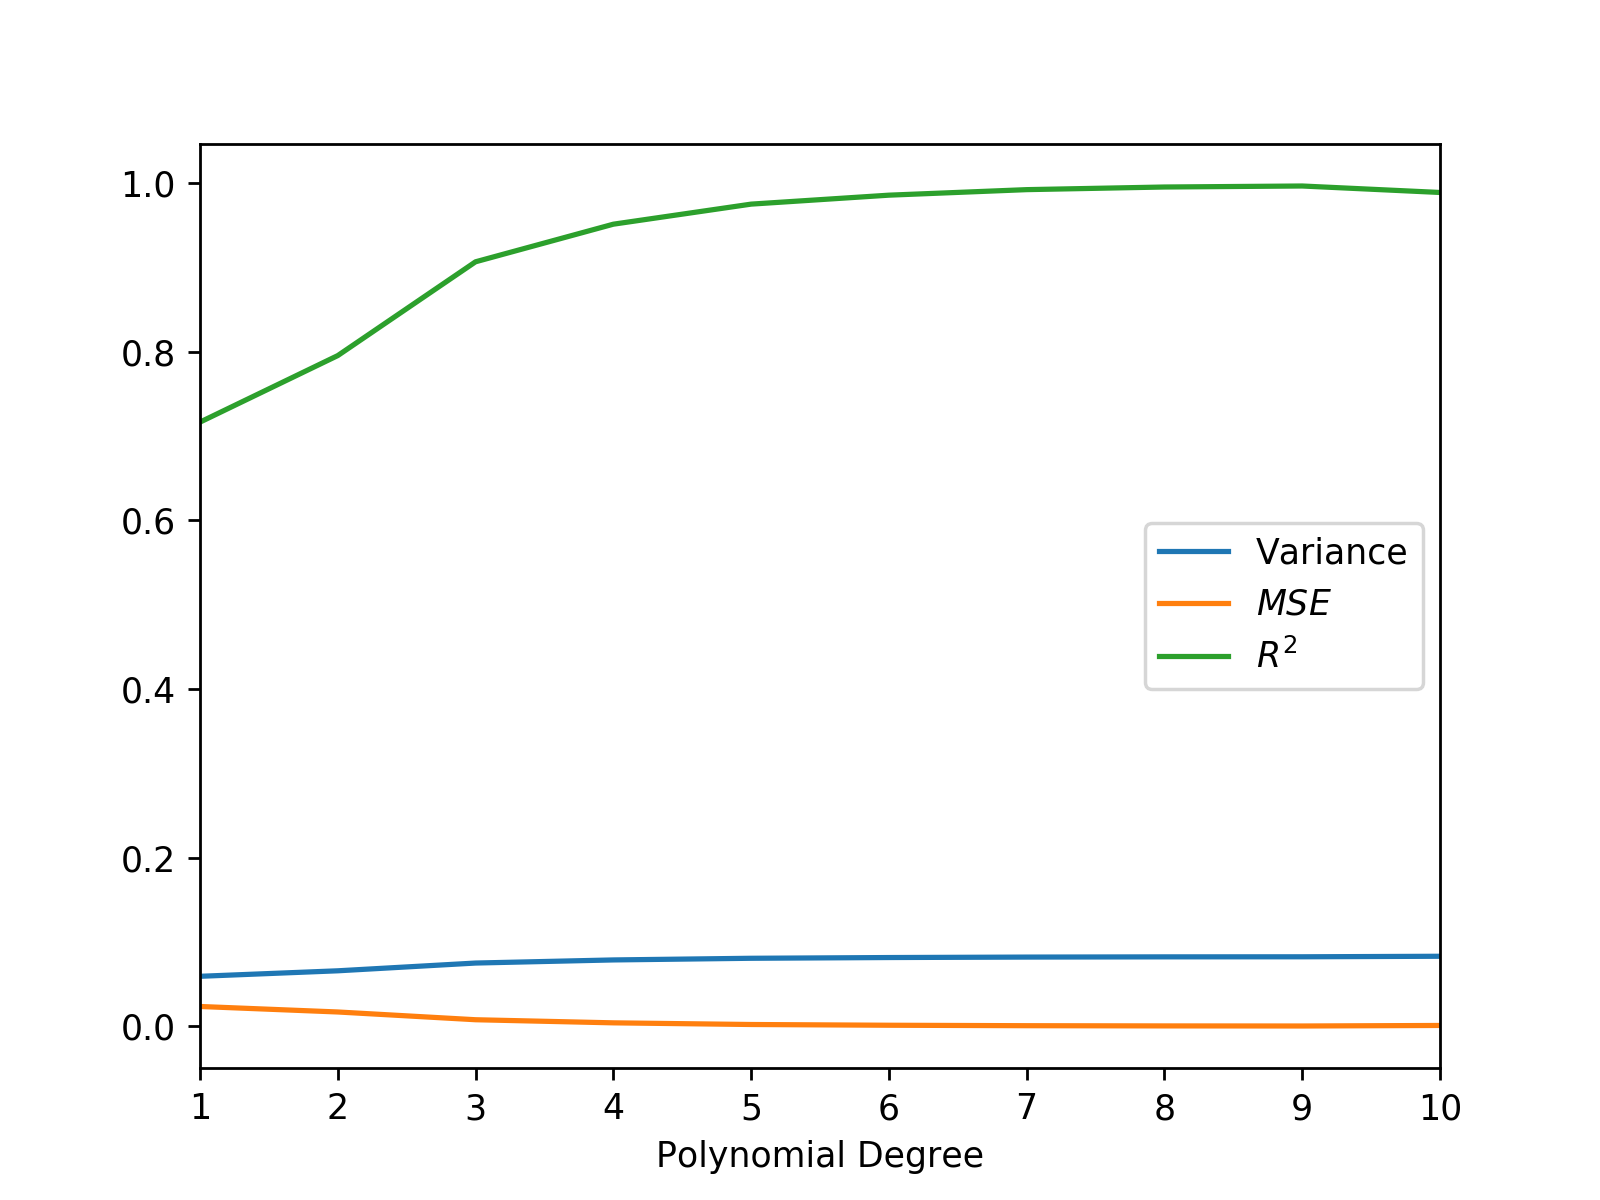
\includegraphics[width = 0.5\textwidth, center]{../franke_output/part_A.png}
	\caption{The $MSE$, the $R^2$-score, and the variance $\sigma$ in the vector of coefficients $\beta$, as functions of the polynomial degree after performing OLS on the Franke-function}
	\label{part_a}
\end{figure}

\begin{figure}[H]
	\centering 
	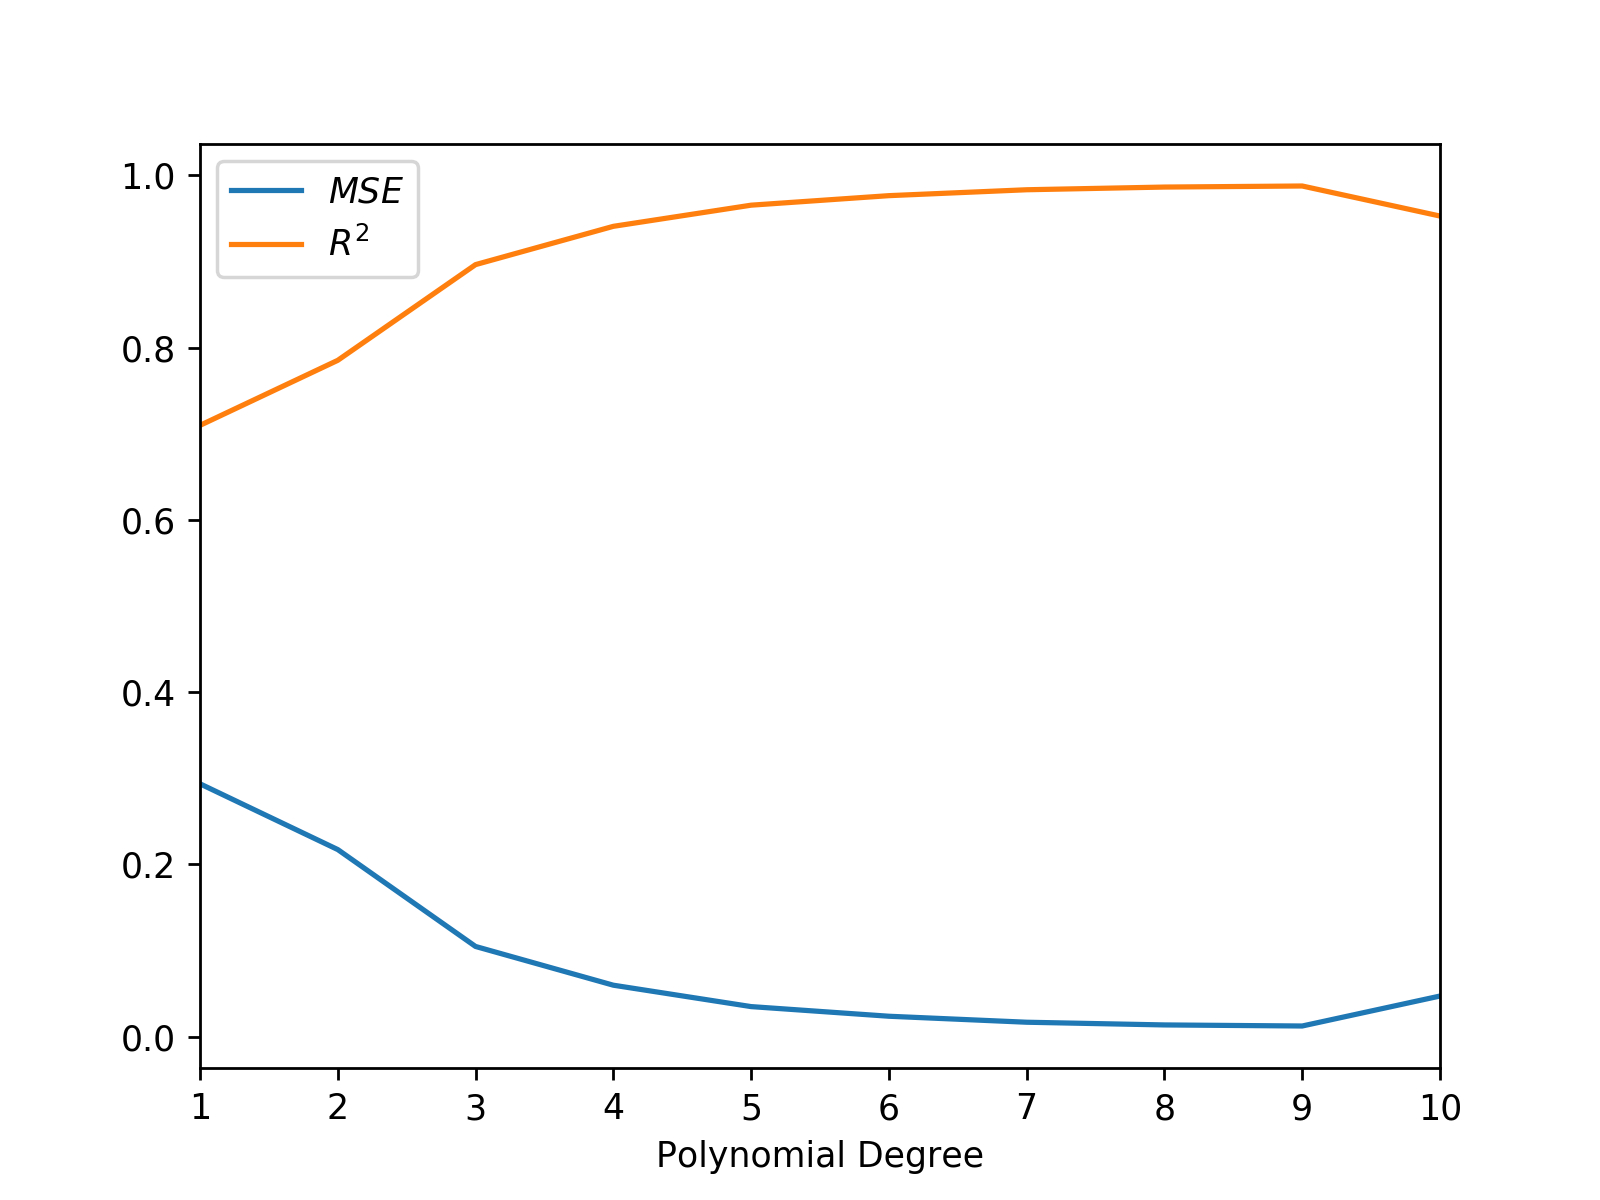
\includegraphics[width = 0.5\textwidth, center]{../franke_output/part_B.png}
	\caption{The $MSE$, the $R^2$-score, and the variance $\sigma$ in the vector of coefficients $\beta$ as functions of the polynomial degree after performing \textit{OLS} on the Franke-function.  Using $12$-fold cross validation.}
	\label{part_b}
\end{figure}

%Part c:

\begin{figure}[H]
	\centering 
	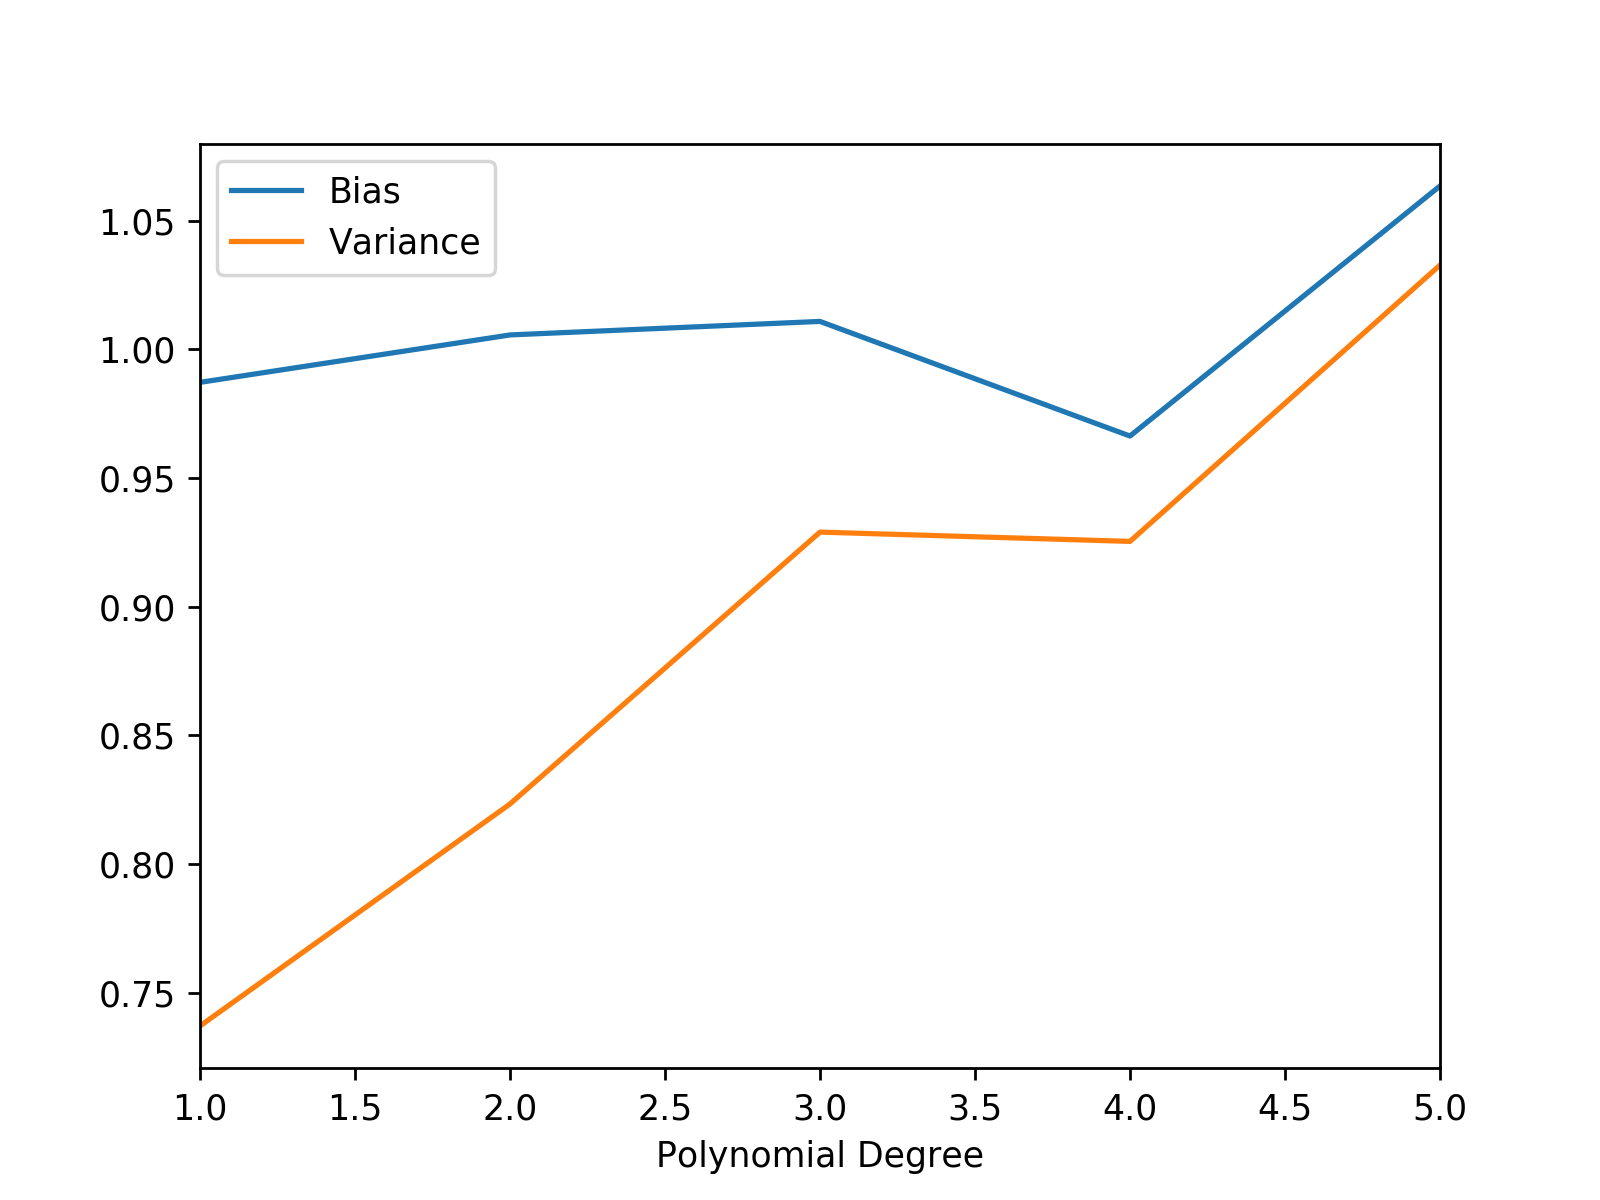
\includegraphics[width = 0.5\textwidth, center]{../franke_output/part_C_1.png}
	\caption{The \textit{bias} and \textit{variance} as functions of the polynomial degree after performing \textit{OLS} on the Franke-function}
	\label{part_c1}
\end{figure}

\begin{figure}[H]
	\centering 
	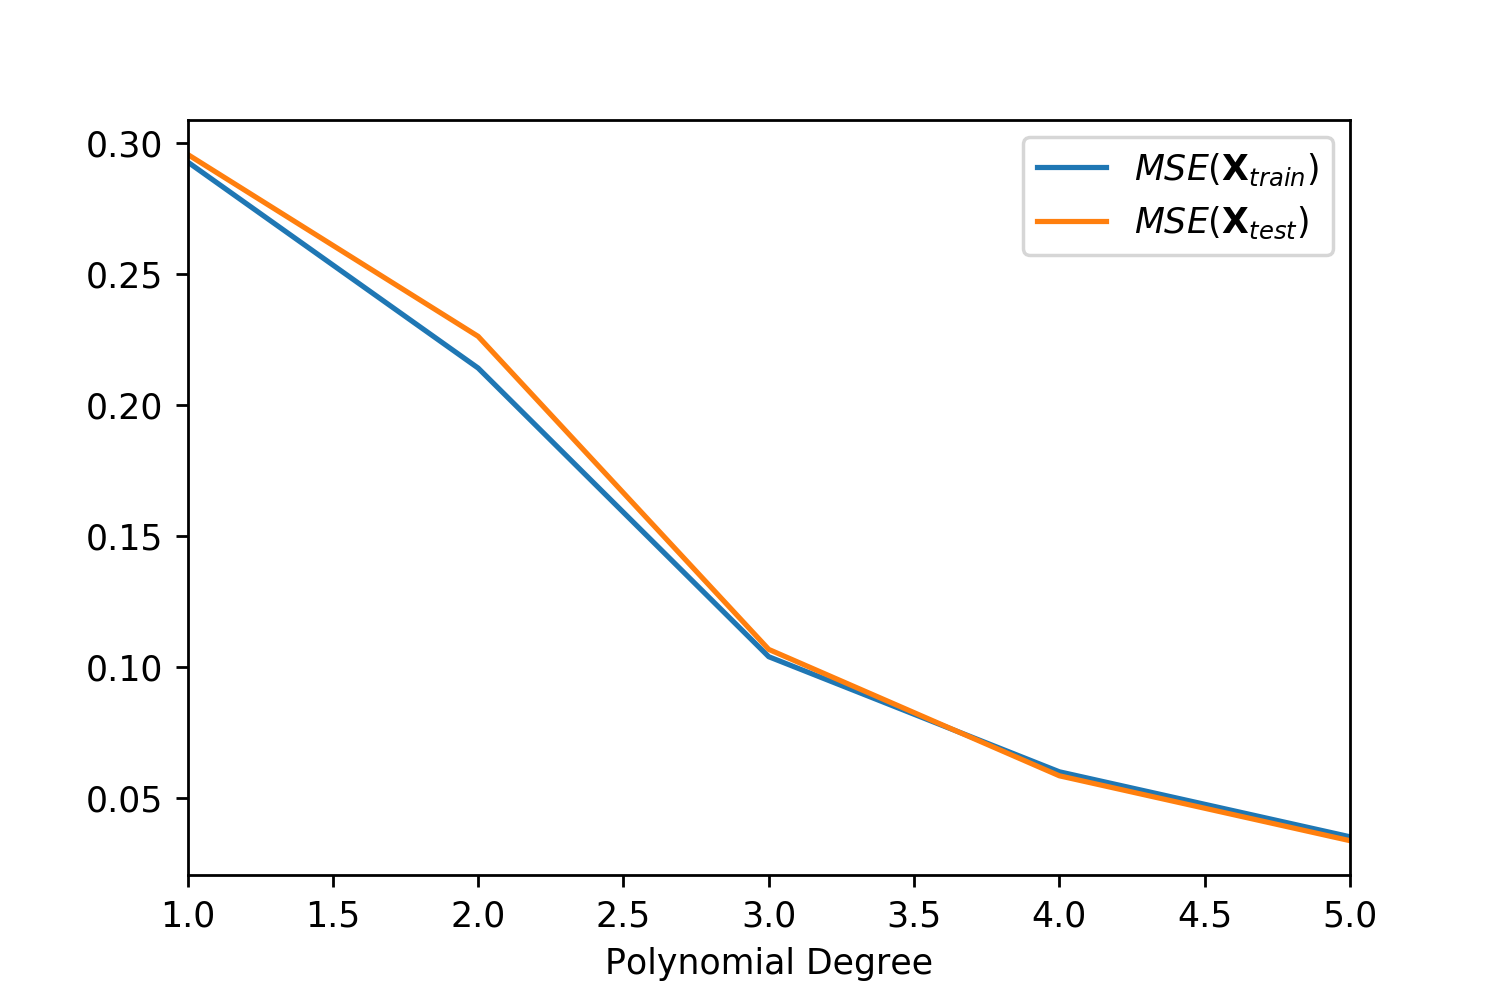
\includegraphics[width = 0.5\textwidth, center]{../franke_output/part_C_2.png}
	\caption{The $MSE$ for the \textit{training data} and the \textit{testing data}, as a function of the polynomial degree after performing \textit{OLS} on the Franke-function}
	\label{part_c2}
\end{figure}

%Part d:

\begin{figure}[H]
	\centering 
	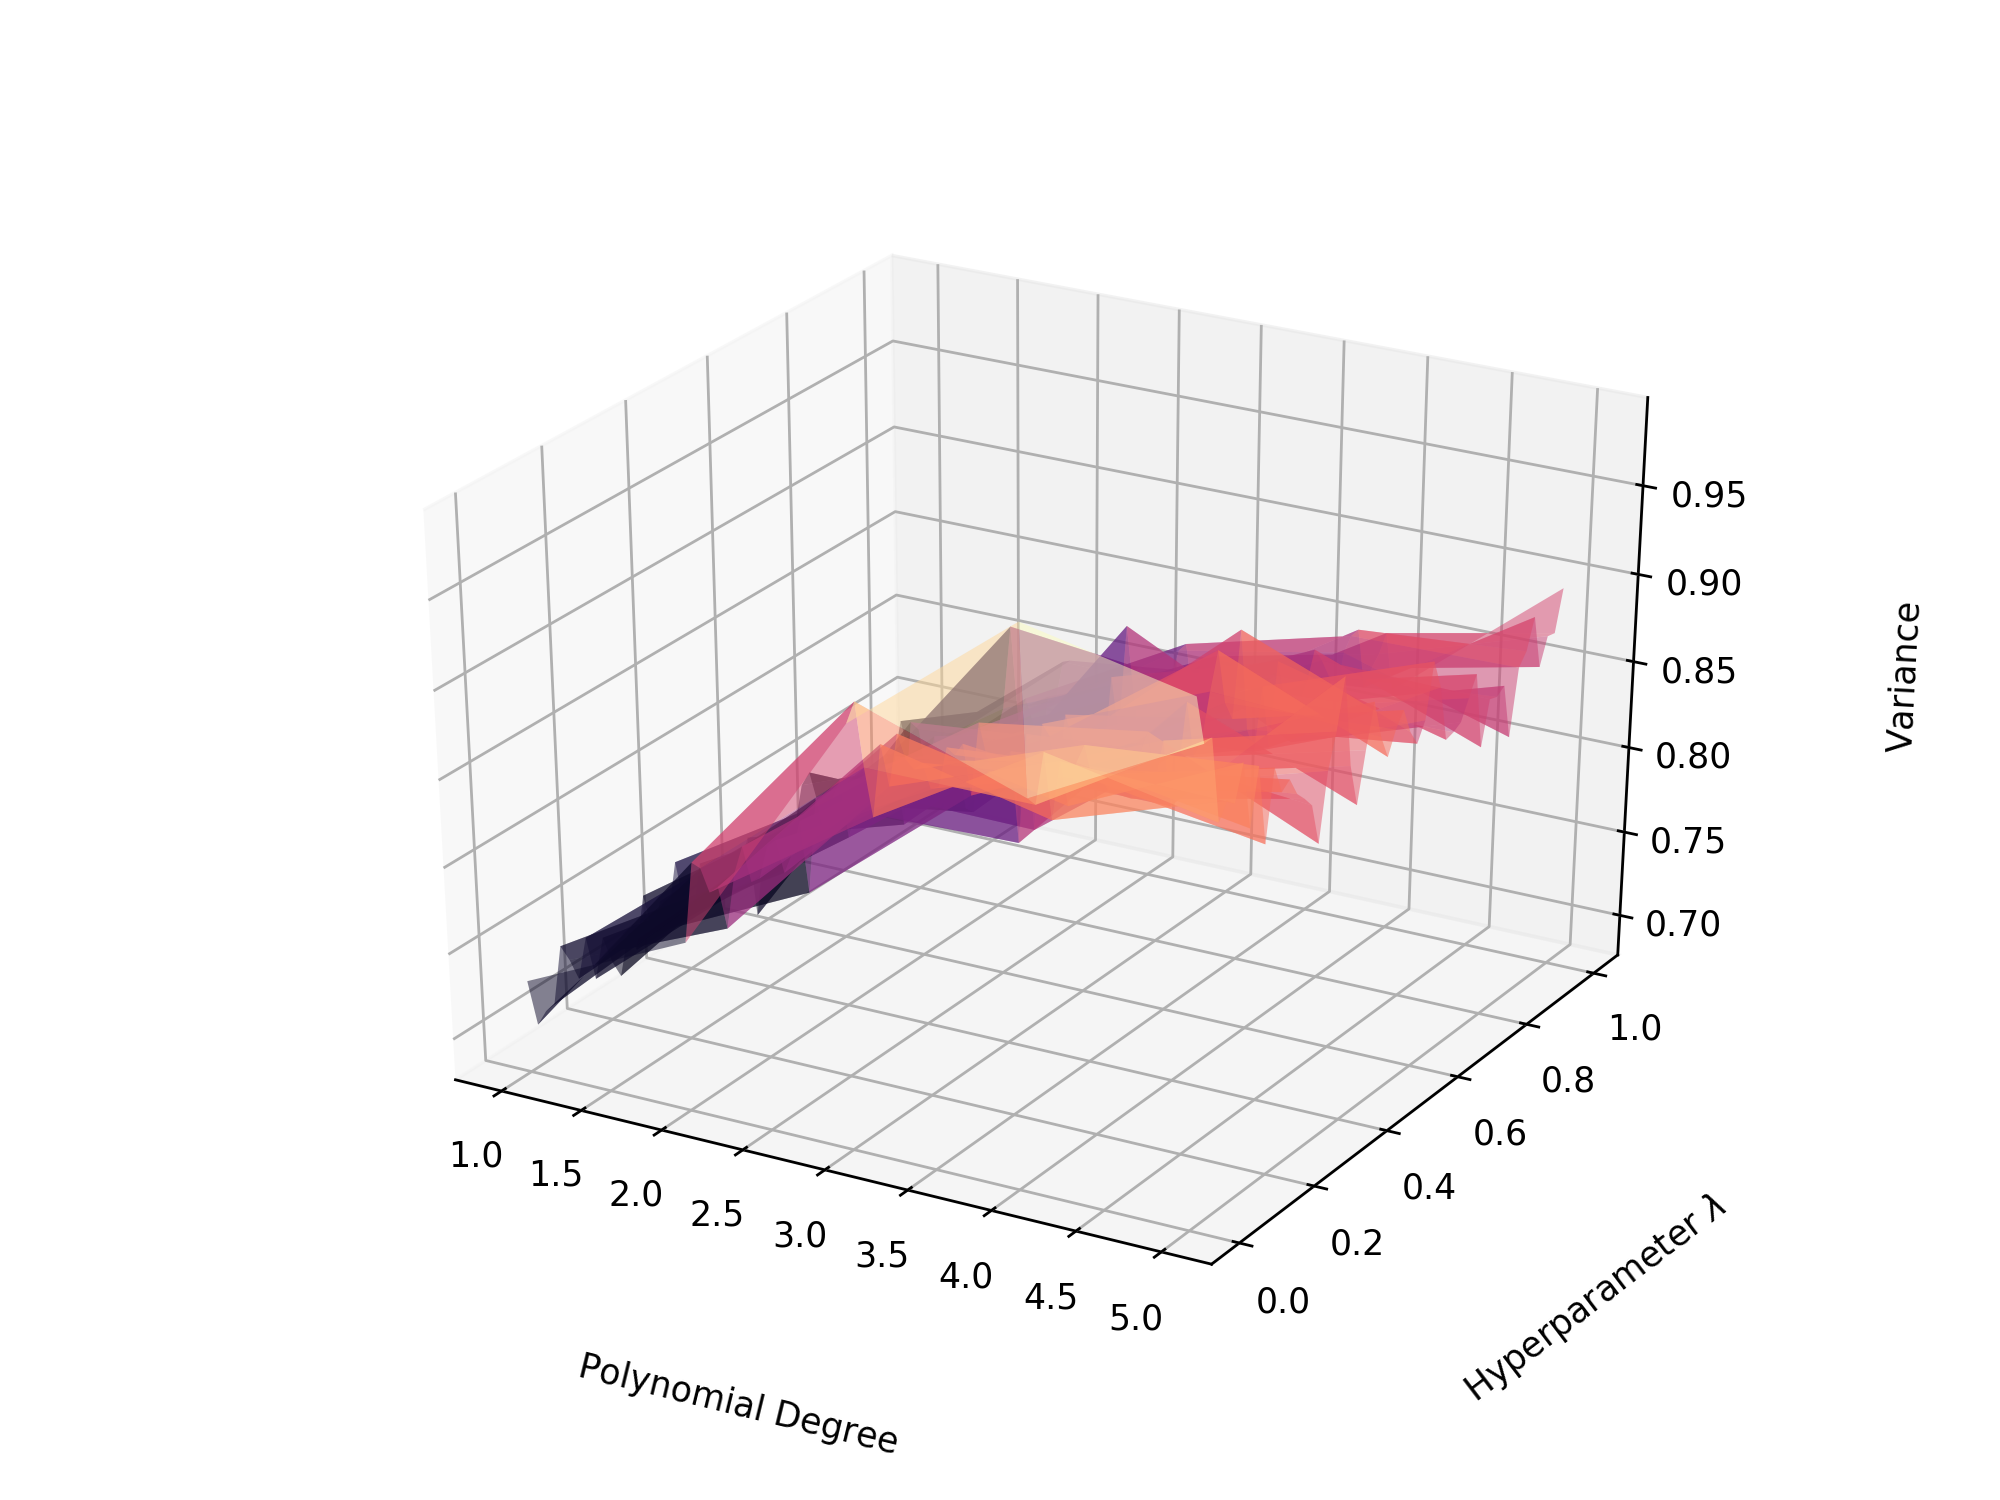
\includegraphics[width = 0.5\textwidth, center]{../franke_output/part_D_1.png}
	\caption{The \textit{variance} as a function of polynomial degree and hyperparameter $\lambda$, after performing \textit{Ridge regression} on the Franke-function}
	\label{part_d1}
\end{figure}

\begin{figure}[H]
	\centering 
	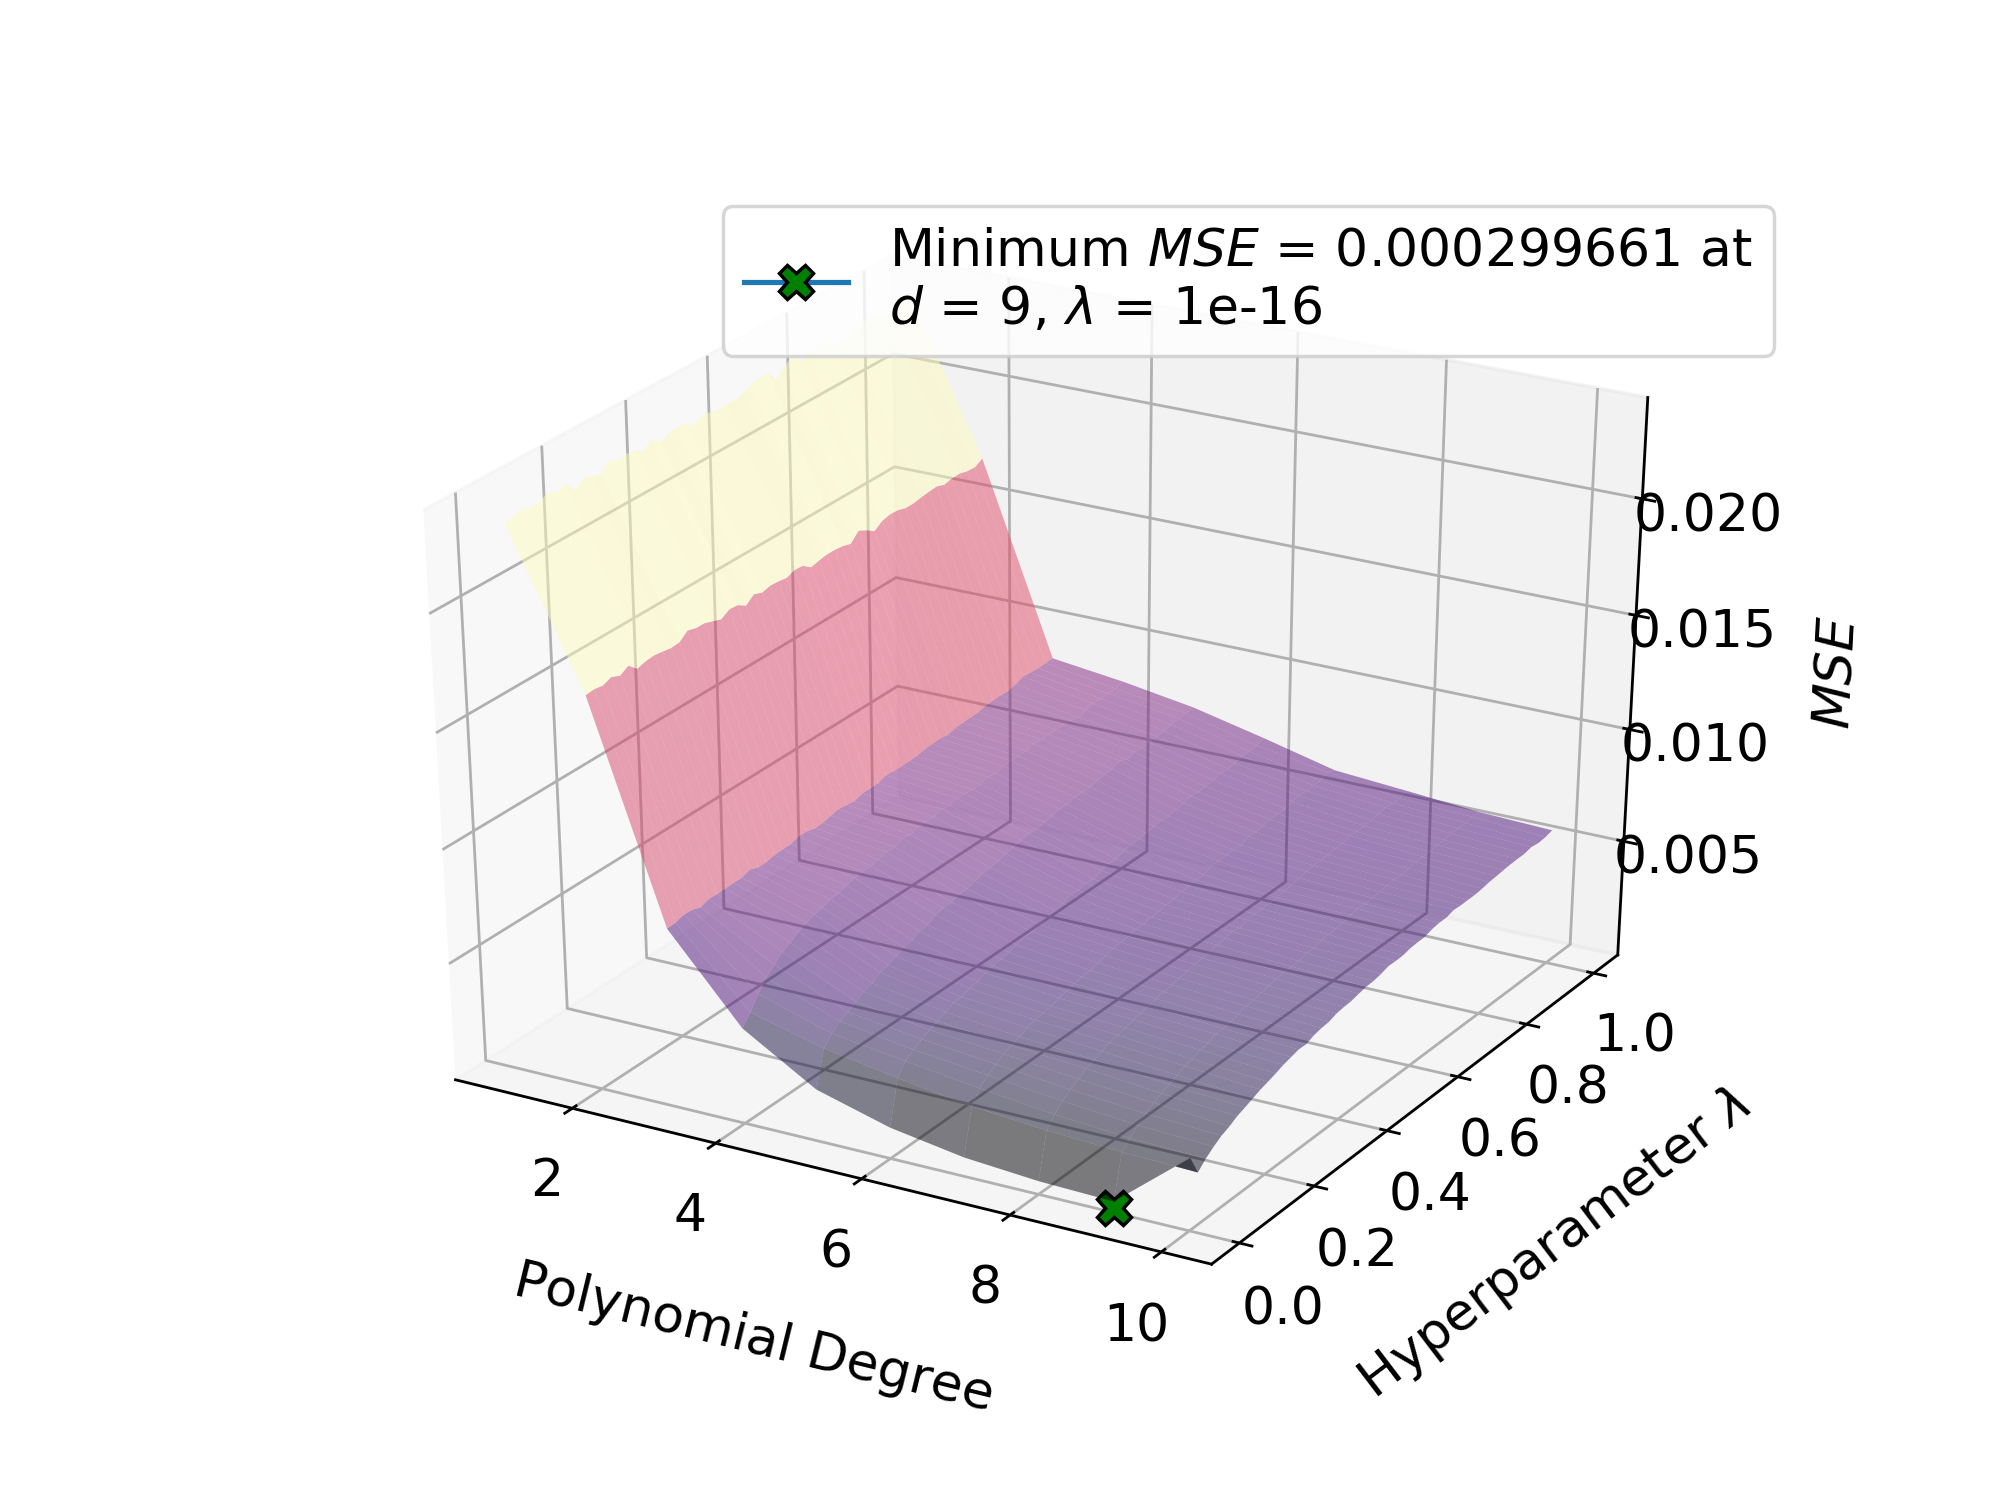
\includegraphics[width = 0.5\textwidth, center]{../franke_output/part_D_2.png}
	\caption{The $MSE$ as a function of the polynomial degree and hyperparameter $\lambda$ after performing \textit{Ridge regression} on the Franke-function}
	\label{part_d2}
\end{figure}

\begin{figure}[H]
	\centering 
	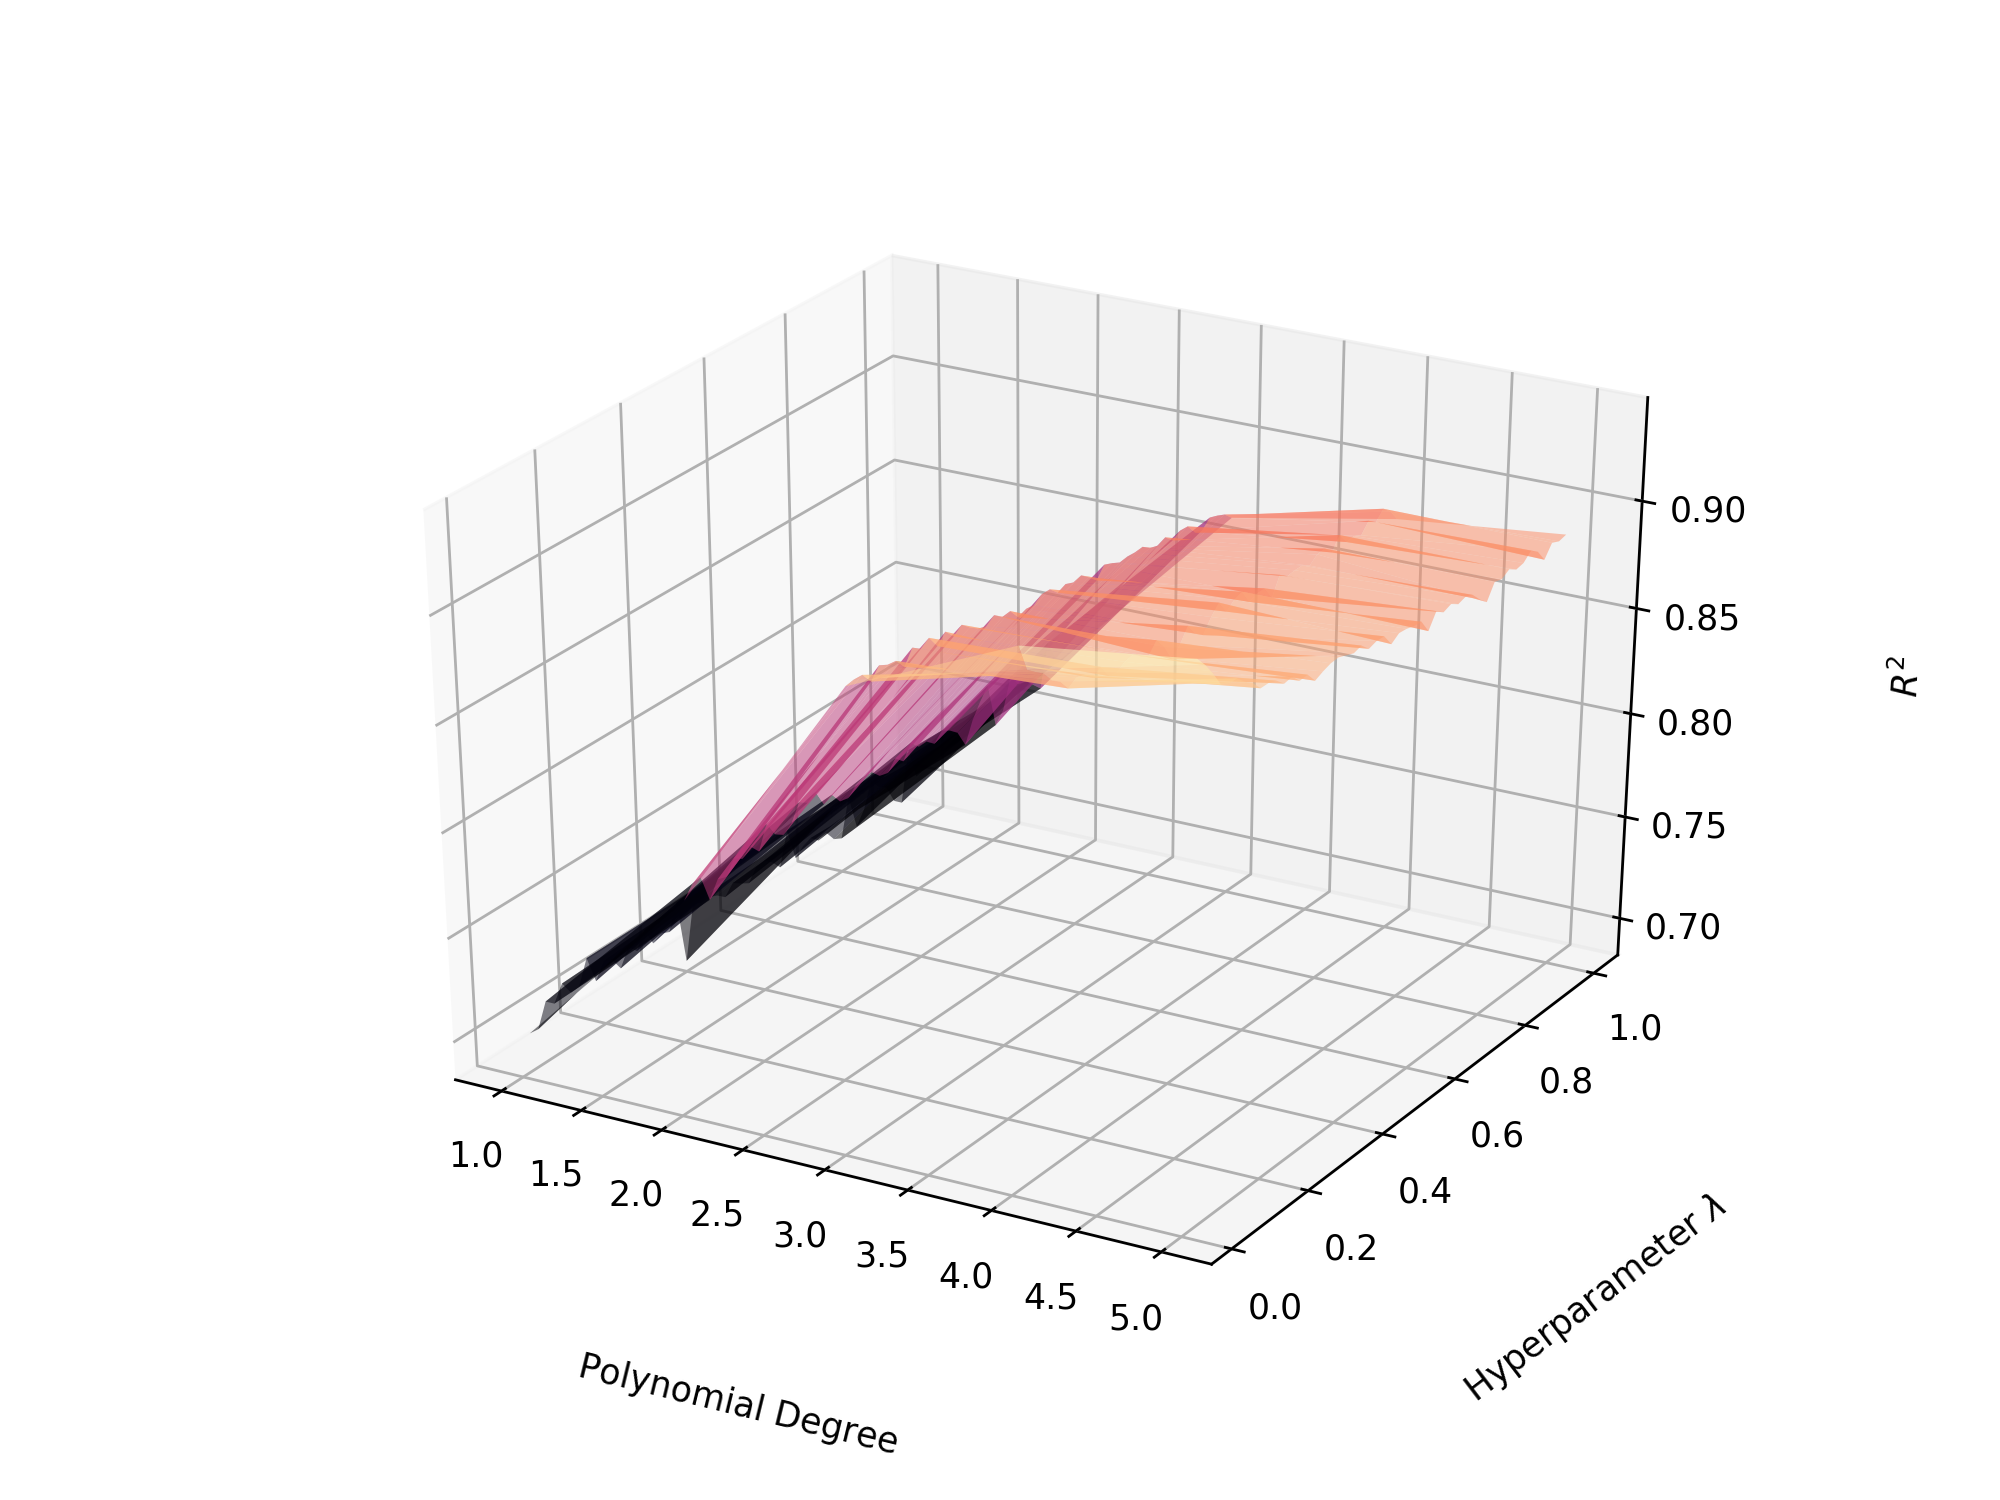
\includegraphics[width = 0.5\textwidth, center]{../franke_output/part_D_3.png}
	\caption{The $R^2$-score as a function of the polynomial degree and hyperparameter $\lambda$ after performing \textit{Ridge regression} on the Franke-function}
	\label{part_d3}
\end{figure}

\begin{figure}[H]
	\centering 
	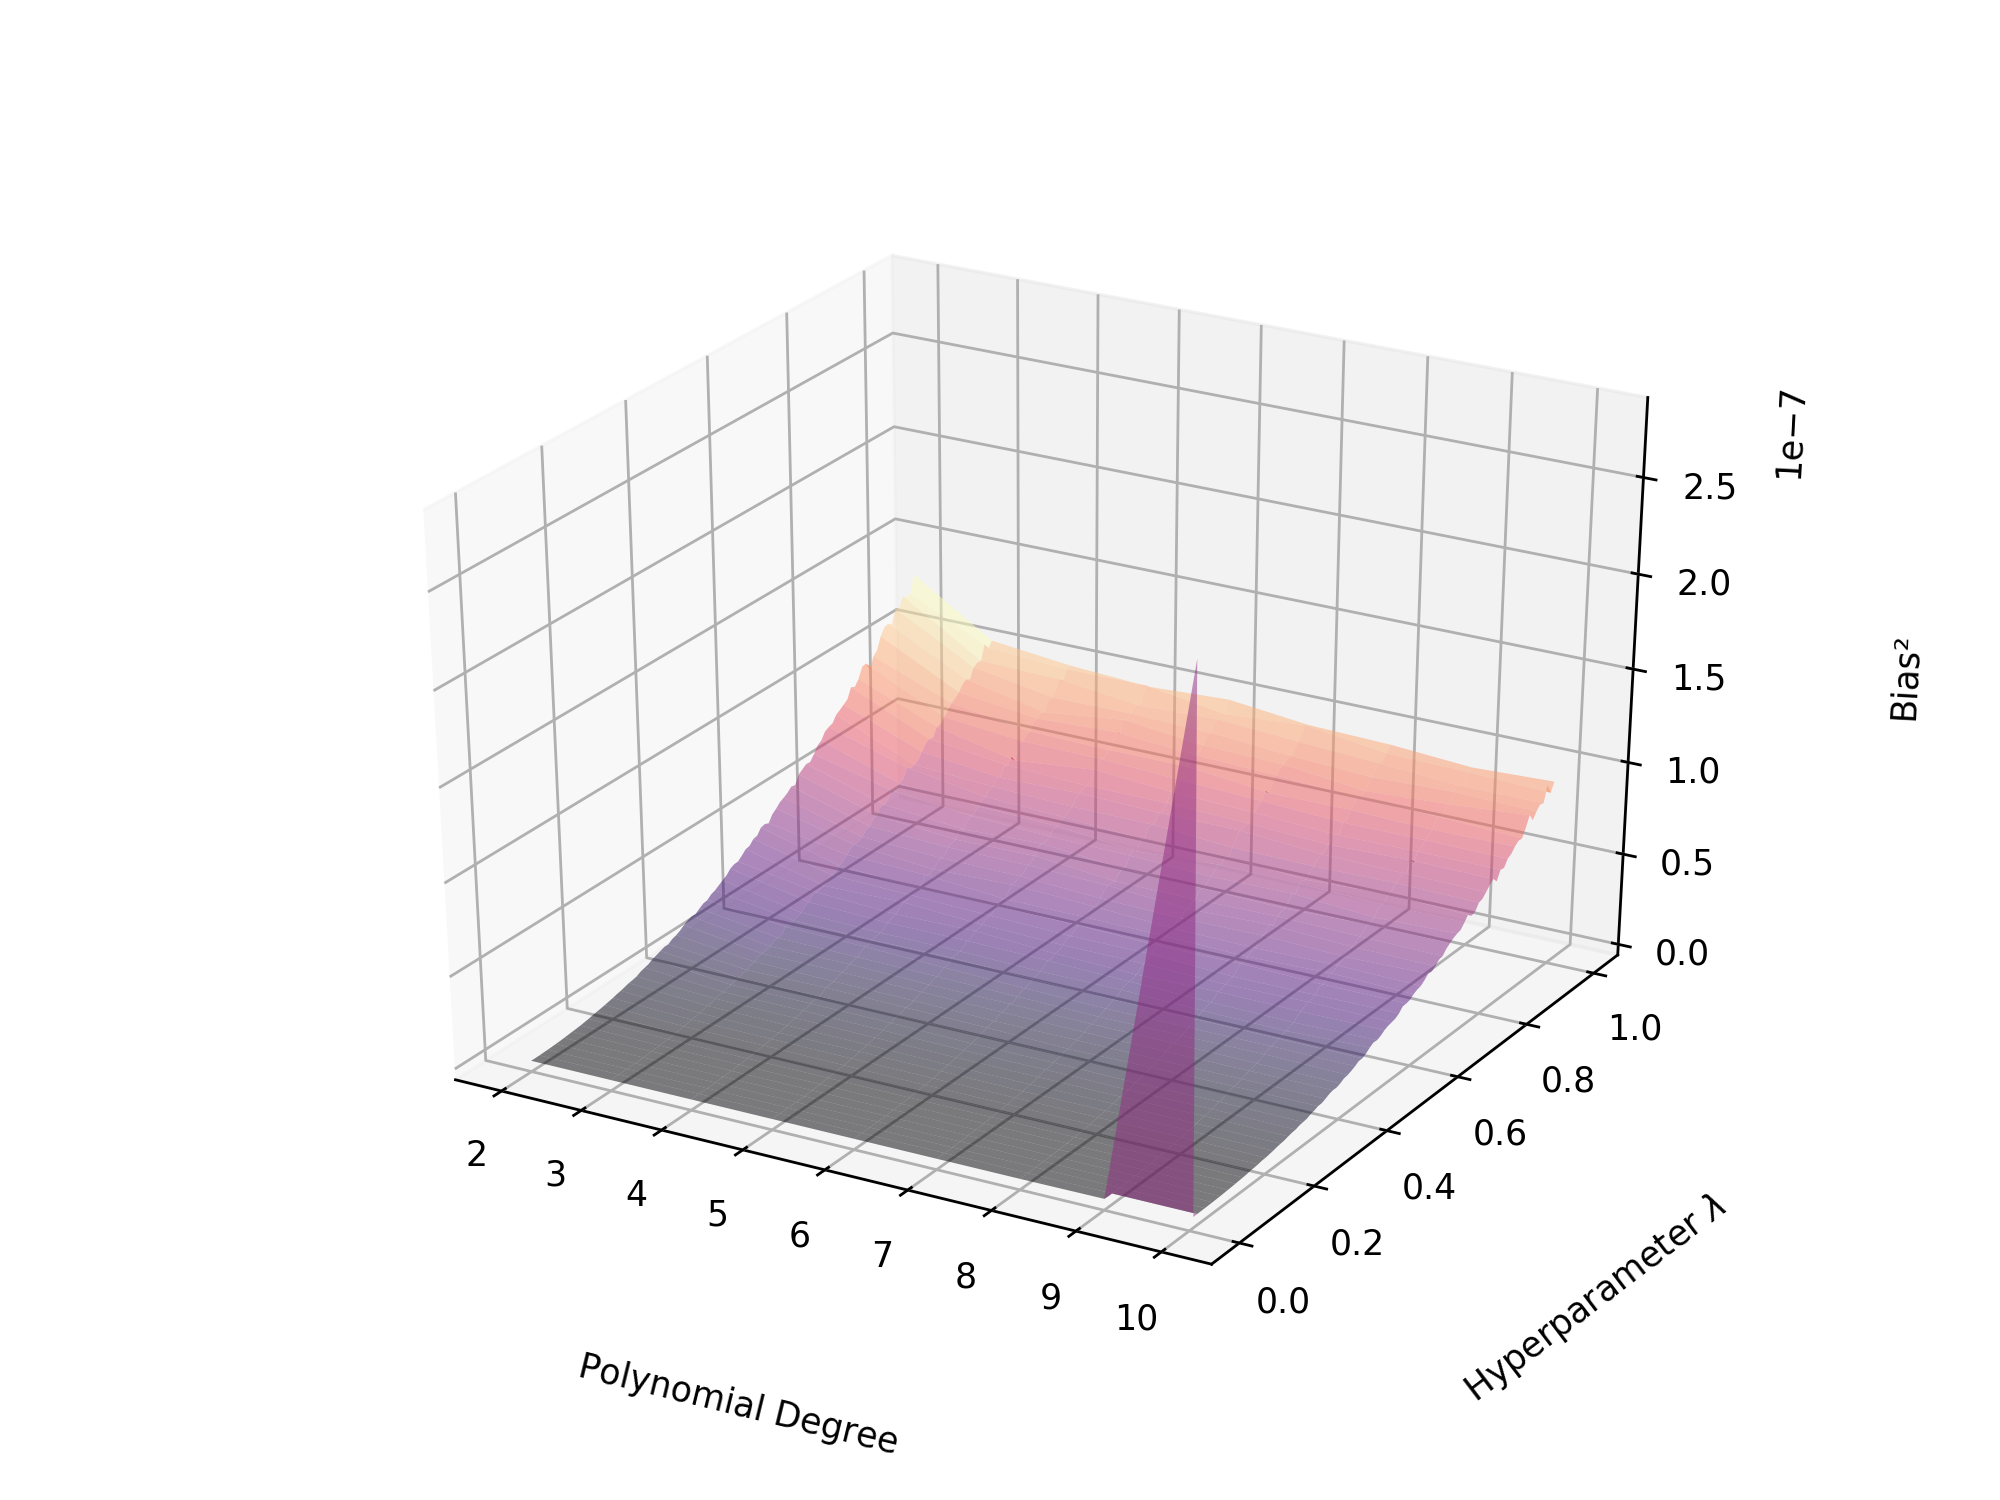
\includegraphics[width = 0.5\textwidth, center]{../franke_output/part_D_4.png}
	\caption{The \textit{squared bias} as a function of the polynomial degree and hyperparameter $\lambda$ after performing \textit{Ridge regression} on the Franke-function}
	\label{part_d4}
\end{figure}

%Part e:

\begin{figure}[H]
	\centering 
	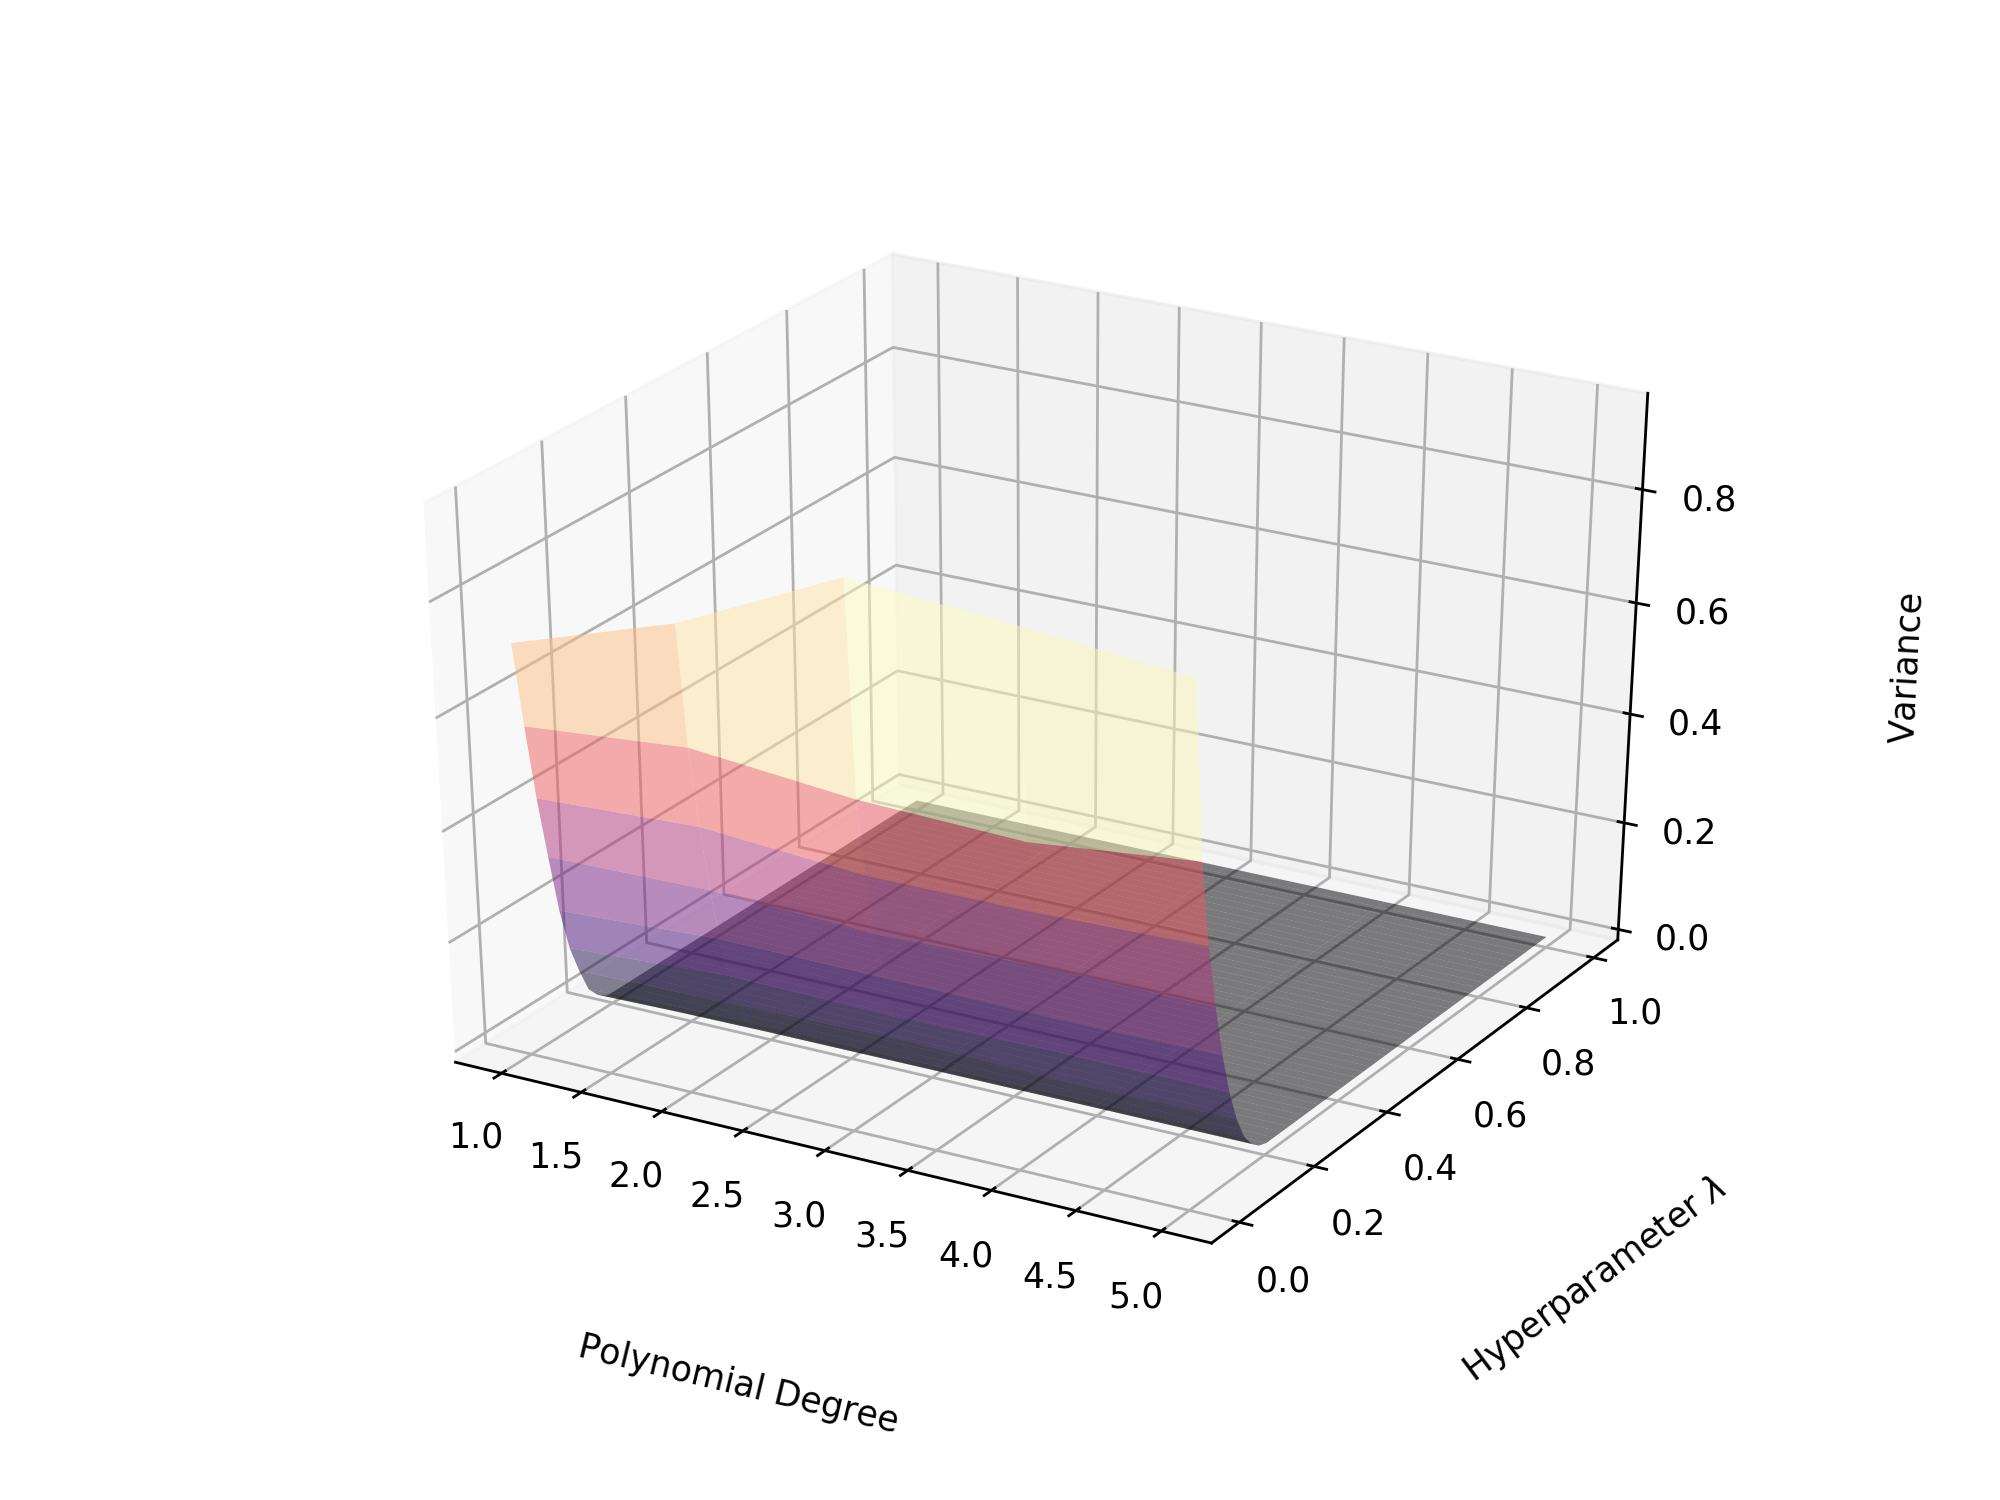
\includegraphics[width = 0.5\textwidth, center]{../franke_output/part_E_1.png}
	\caption{The \textit{variance} as a function of the polynomial degree and hyperparameter $\lambda$ after performing \textit{LASSO regression} on the Franke-function}
	\label{part_e1}
\end{figure}

\begin{figure}[H]
	\centering 
	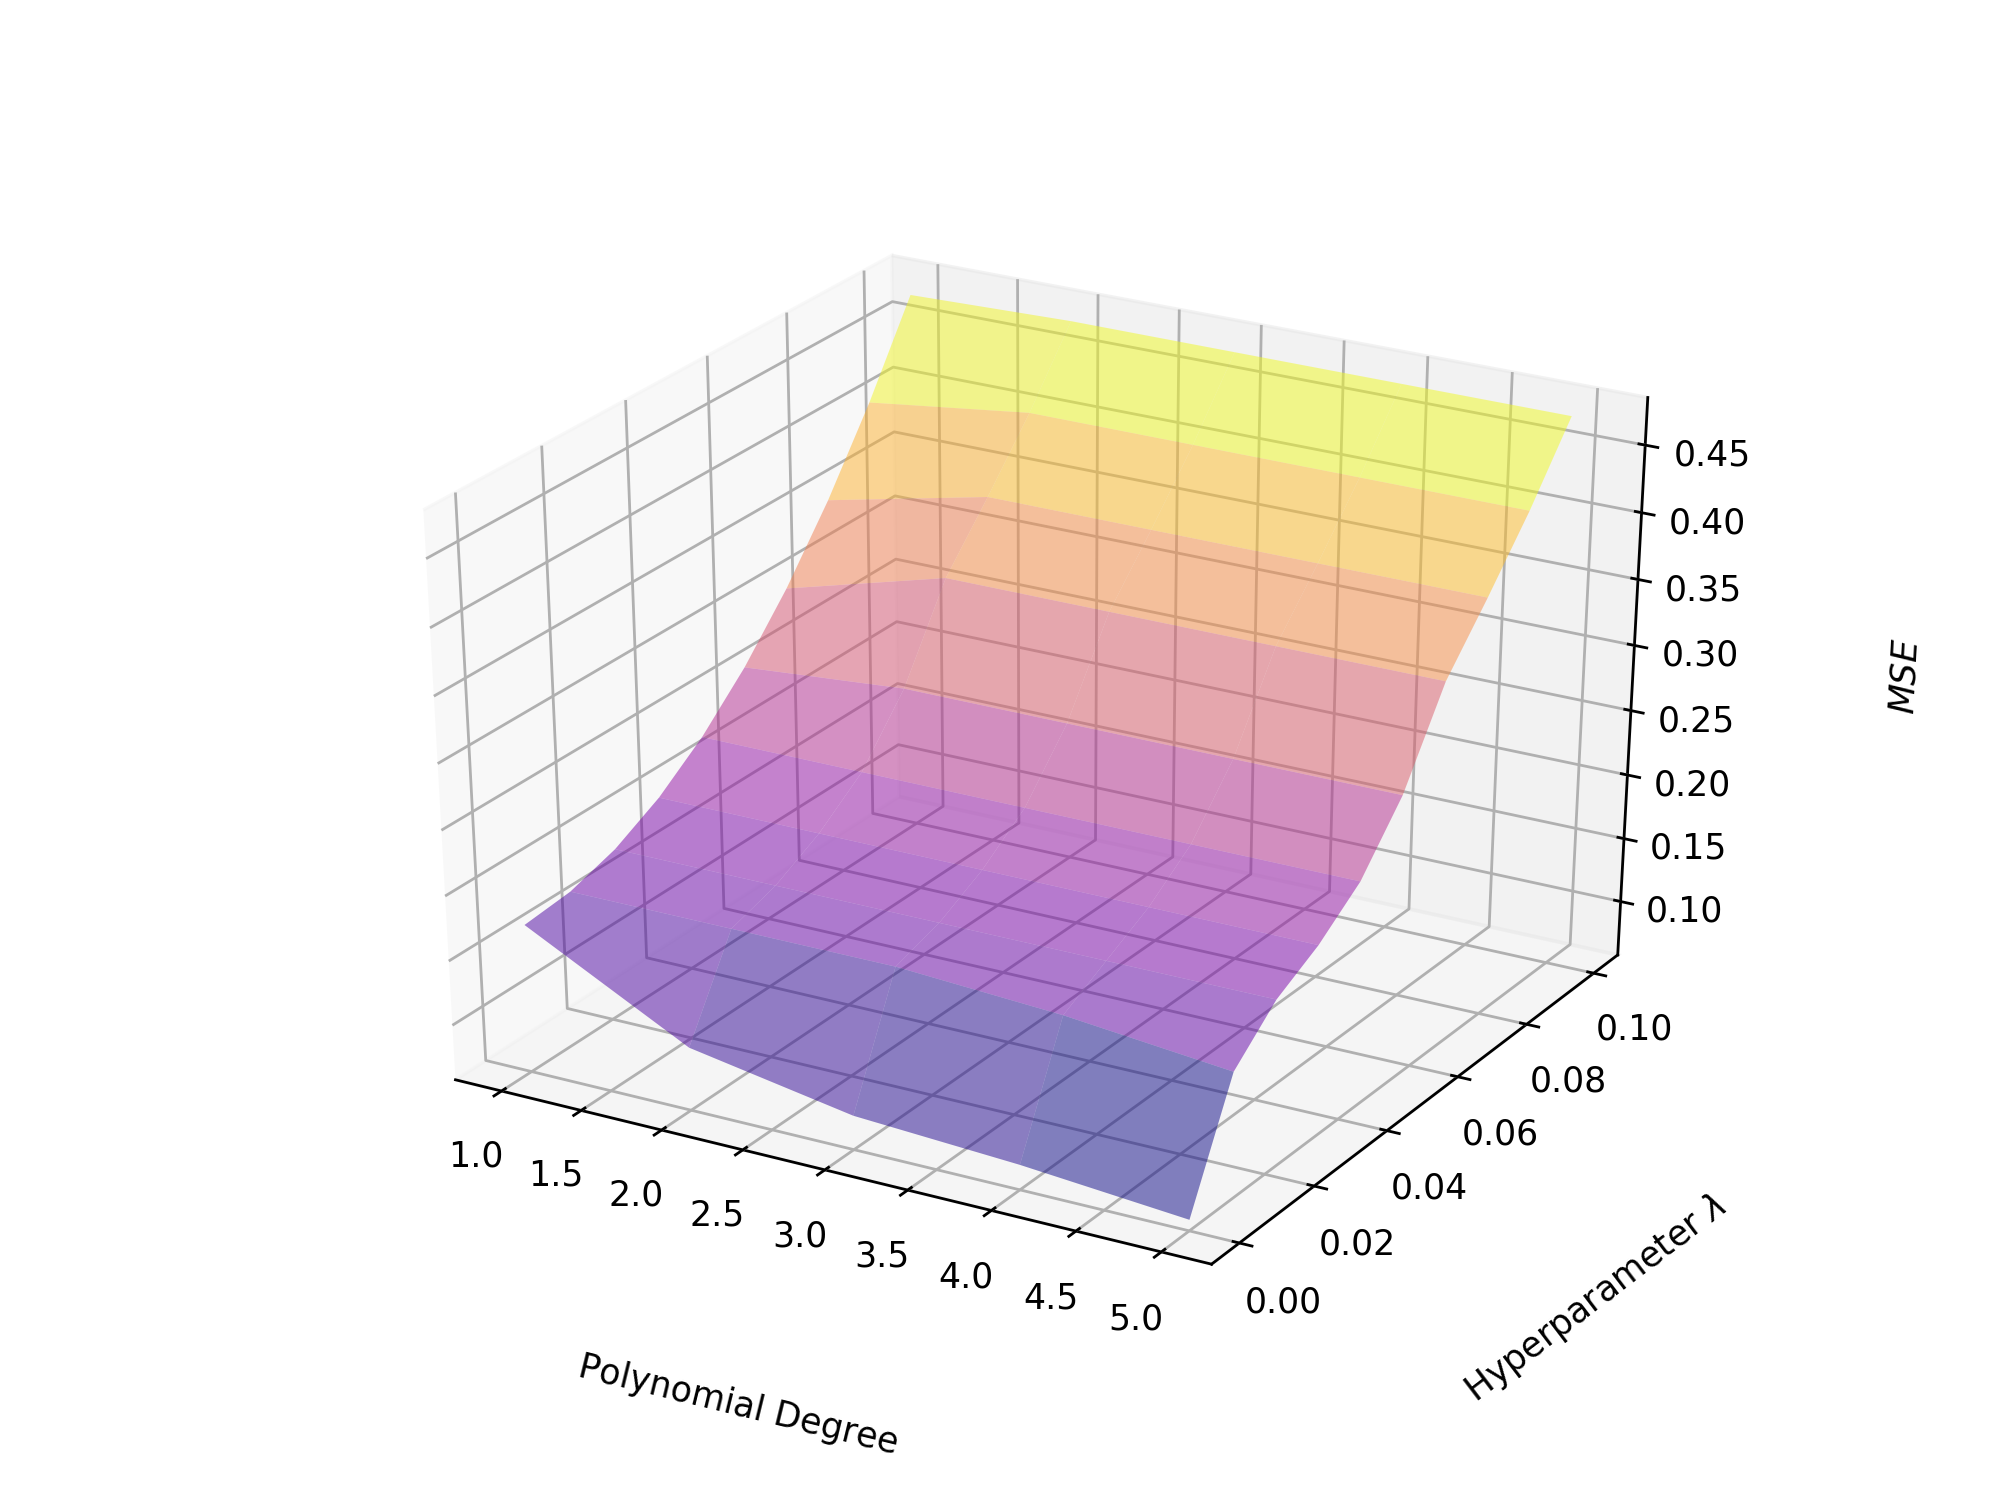
\includegraphics[width = 0.5\textwidth, center]{../franke_output/part_E_2.png}
	\caption{The $MSE$ as a function of the polynomial degree and hyperparameter $\lambda$ after performing \textit{LASSO regression} on the Franke-function}
	\label{part_e2}
\end{figure}

\begin{figure}[H]
	\centering 
	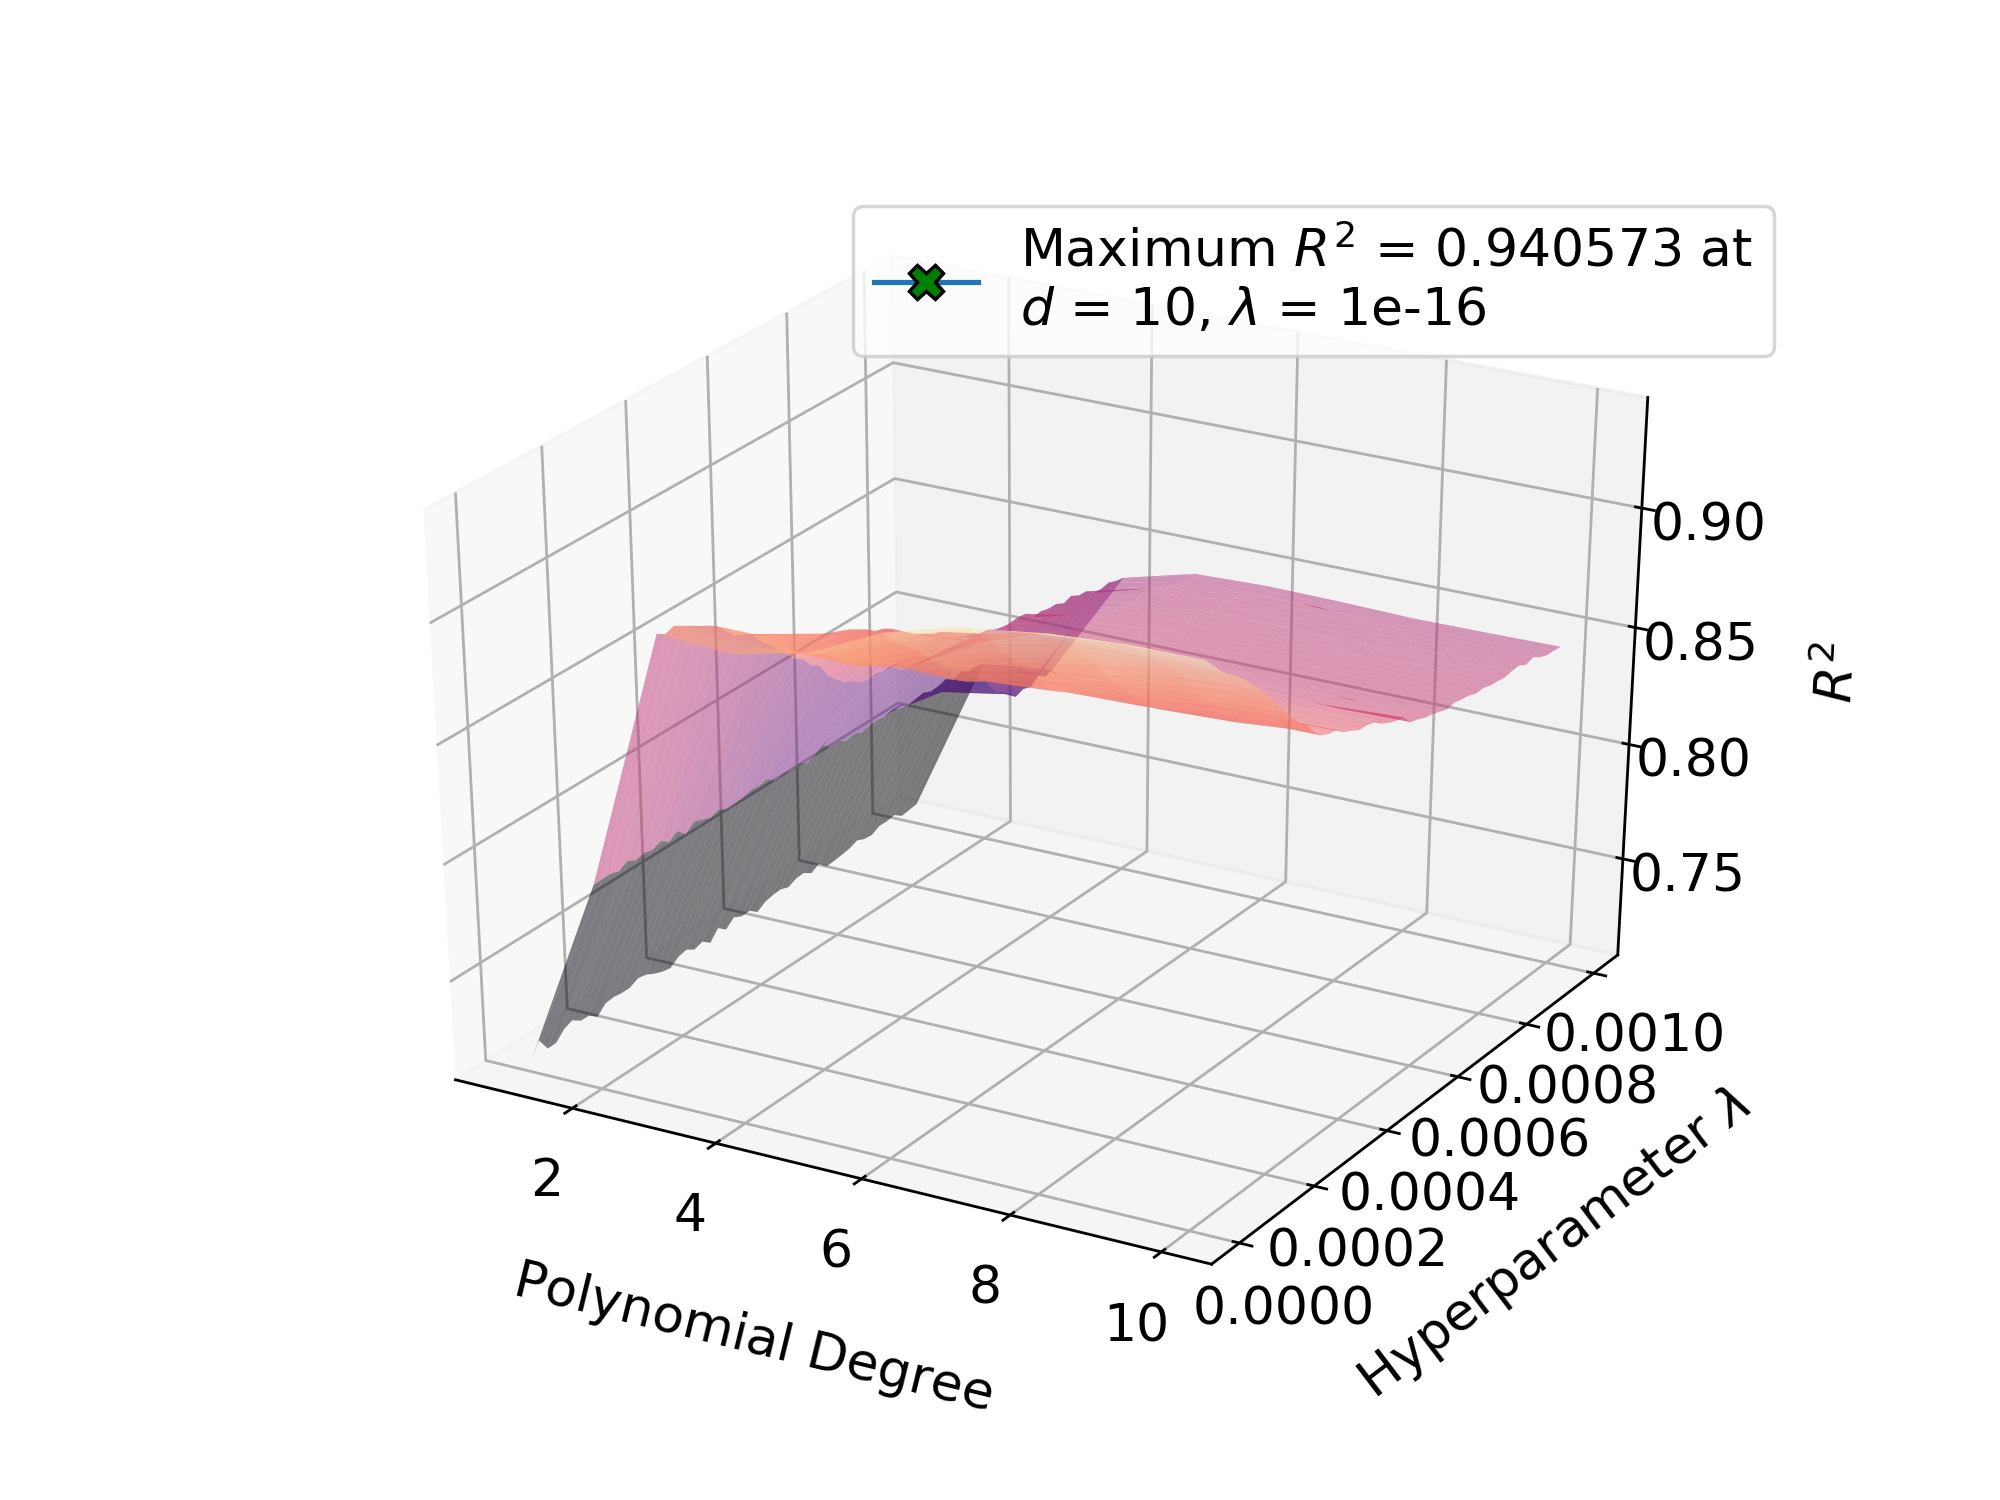
\includegraphics[width = 0.5\textwidth, center]{../franke_output/part_E_3.png}
	\caption{The $R^2$-score as a function of the polynomial degree and hyperparameter $\lambda$ after performing \textit{LASSO regression} on the Franke-function}
	\label{part_e3}
\end{figure}

\begin{figure}[H]
	\centering 
	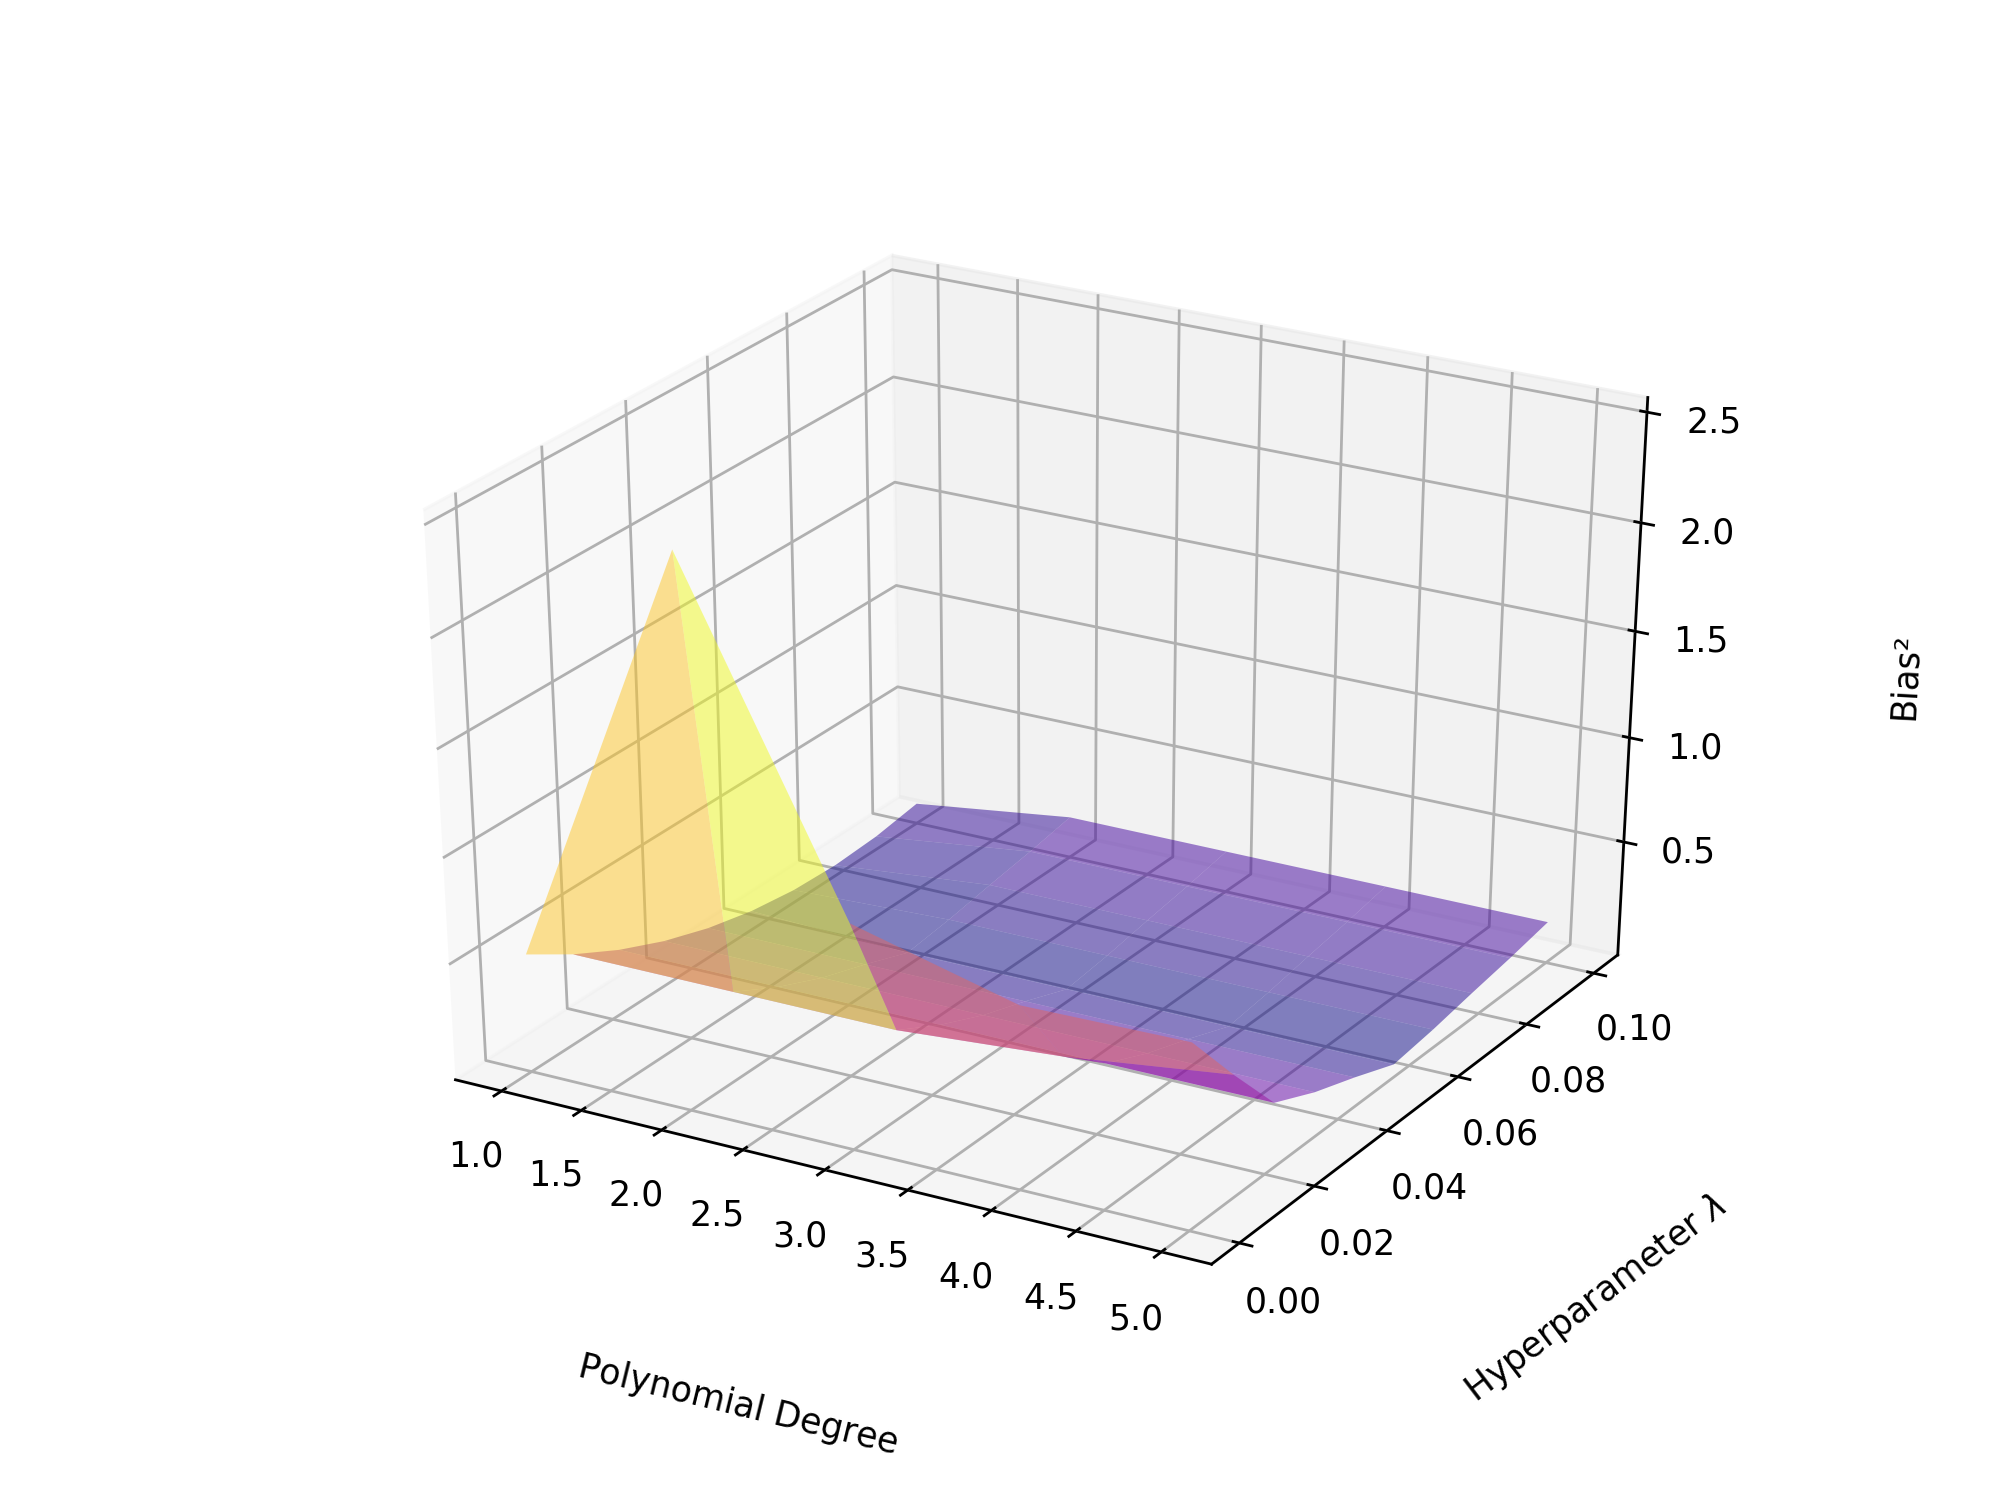
\includegraphics[width = 0.5\textwidth, center]{../franke_output/part_E_4.png}
	\caption{The \textit{squared bias} as a function of the polynomial degree and hyperparameter $\lambda$ after performing \textit{LASSO regression} on the Franke-function}
	\label{part_e4}
\end{figure}



%part g

\subsection{Real Data}


Following bellow is several plots we made of our result after studying regression on the real terrain data. All the plots shows the results for 1 to 10 polynomil degrees.

Figure \ref{part_g_a} to \ref{part_g_c2} details the ordinary least square method.
Figure \ref{part_g_a} shows the variance, mean square error and the $R^2$-score.
Figure \ref{part_g_b} shows the mean square error and the $R^2$-score after performing $k$-fold cross validation. 
Figure \ref{part_g_c2} compares the MSE of the training set and the testing set.

Figure \ref{part_g_d1} to \ref{part_g_d3} details the Ridge method. Here we also have plotted the results with $\lambda$ differing between $10^{-10}$ and $1$.
Figure \ref{part_g_d1} shows the varinace.
Figure \ref{part_g_d2} shows the mean squared error, as well as where the minimum value was found.
Figure \ref{part_g_d3} shows the $R^2$-score.

Figure \ref{part_g_e1} to \ref{part_g_e3} details the LASSO method. Here we also have plotted the results with $\lambda$ differing between $10^{-10}$ and $1$.
Figure \ref{part_g_e1} shows the varinace.
Figure \ref{part_g_e2} shows the mean squared error, as well as where the minimum value was found.
Figure \ref{part_g_e3} shows the $R^2$-score.



%Part a and b:

\begin{figure}[H]
	\centering 
	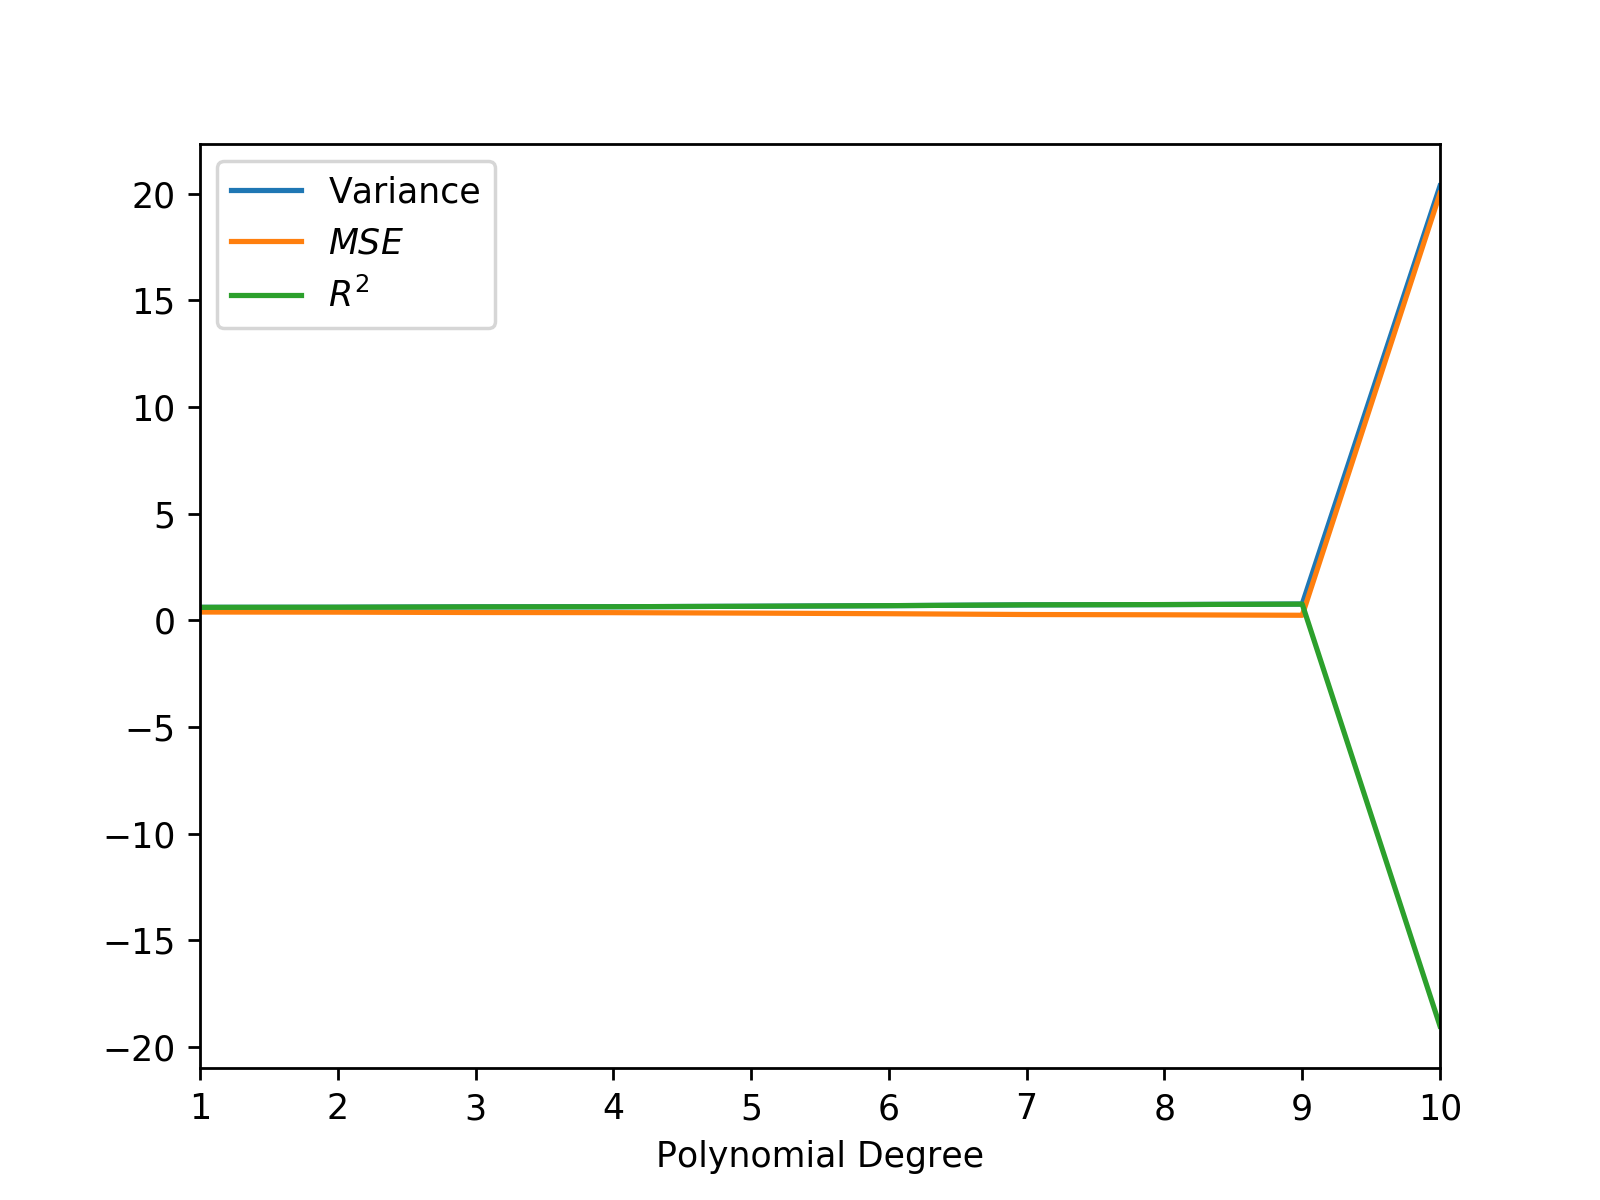
\includegraphics[width = 0.5\textwidth, center]{../real_output/part_A.png}
	\caption{The $MSE$, $R^2$-score and variance $\sigma$ of the vector of coefficients $\beta$ as a function of the polynomial degree after performing \textit{OLS} on real terrain data from \textit{Møsvatn Austfjell}}
	\label{part_g_a}
\end{figure}

\begin{figure}[H]
	\centering 
	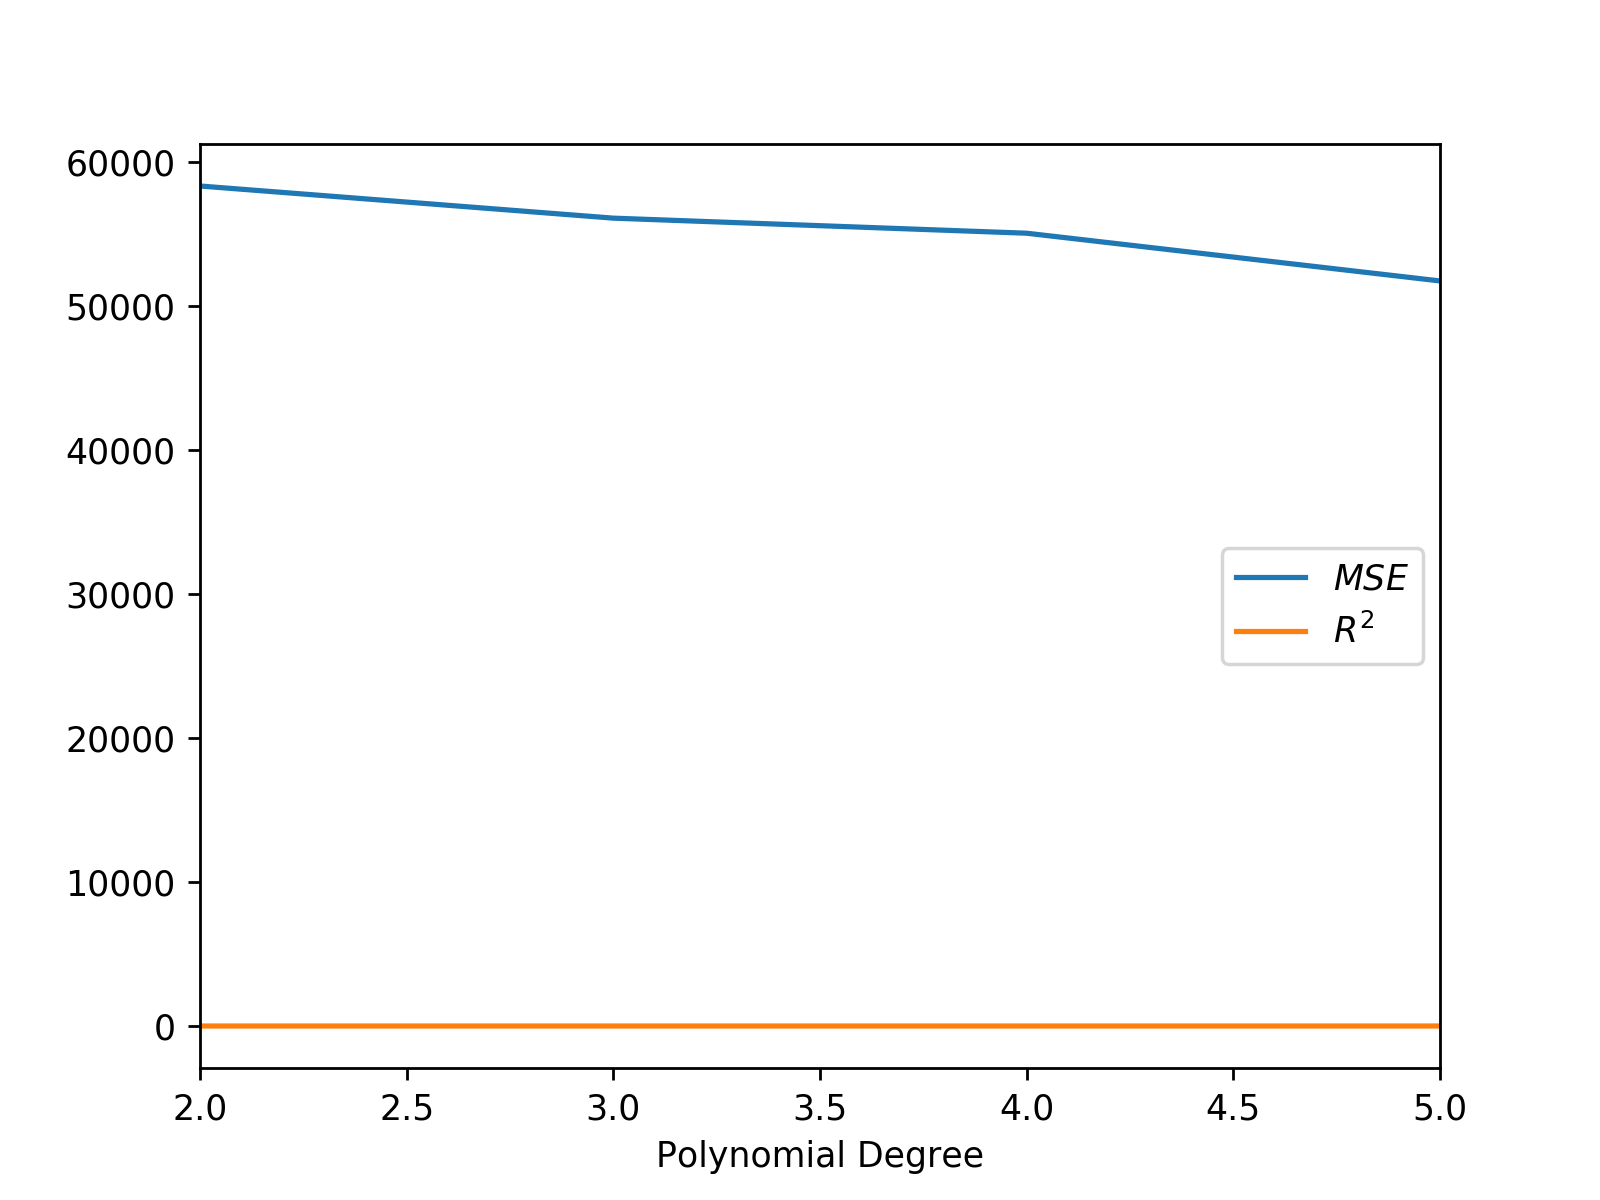
\includegraphics[width = 0.5\textwidth, center]{../real_output/part_B.png}
	\caption{The $MSE$, $R^2$-score and variance $\sigma$ of the vector of coefficients $\beta$ as a function of the polynomial degree after performing \textit{OLS} on real terrain data from \textit{Møsvatn Austfjell}. Using $12$-fold cross validation.}
	\label{part_g_b}
\end{figure}

\begin{figure}[H]
	\centering 
	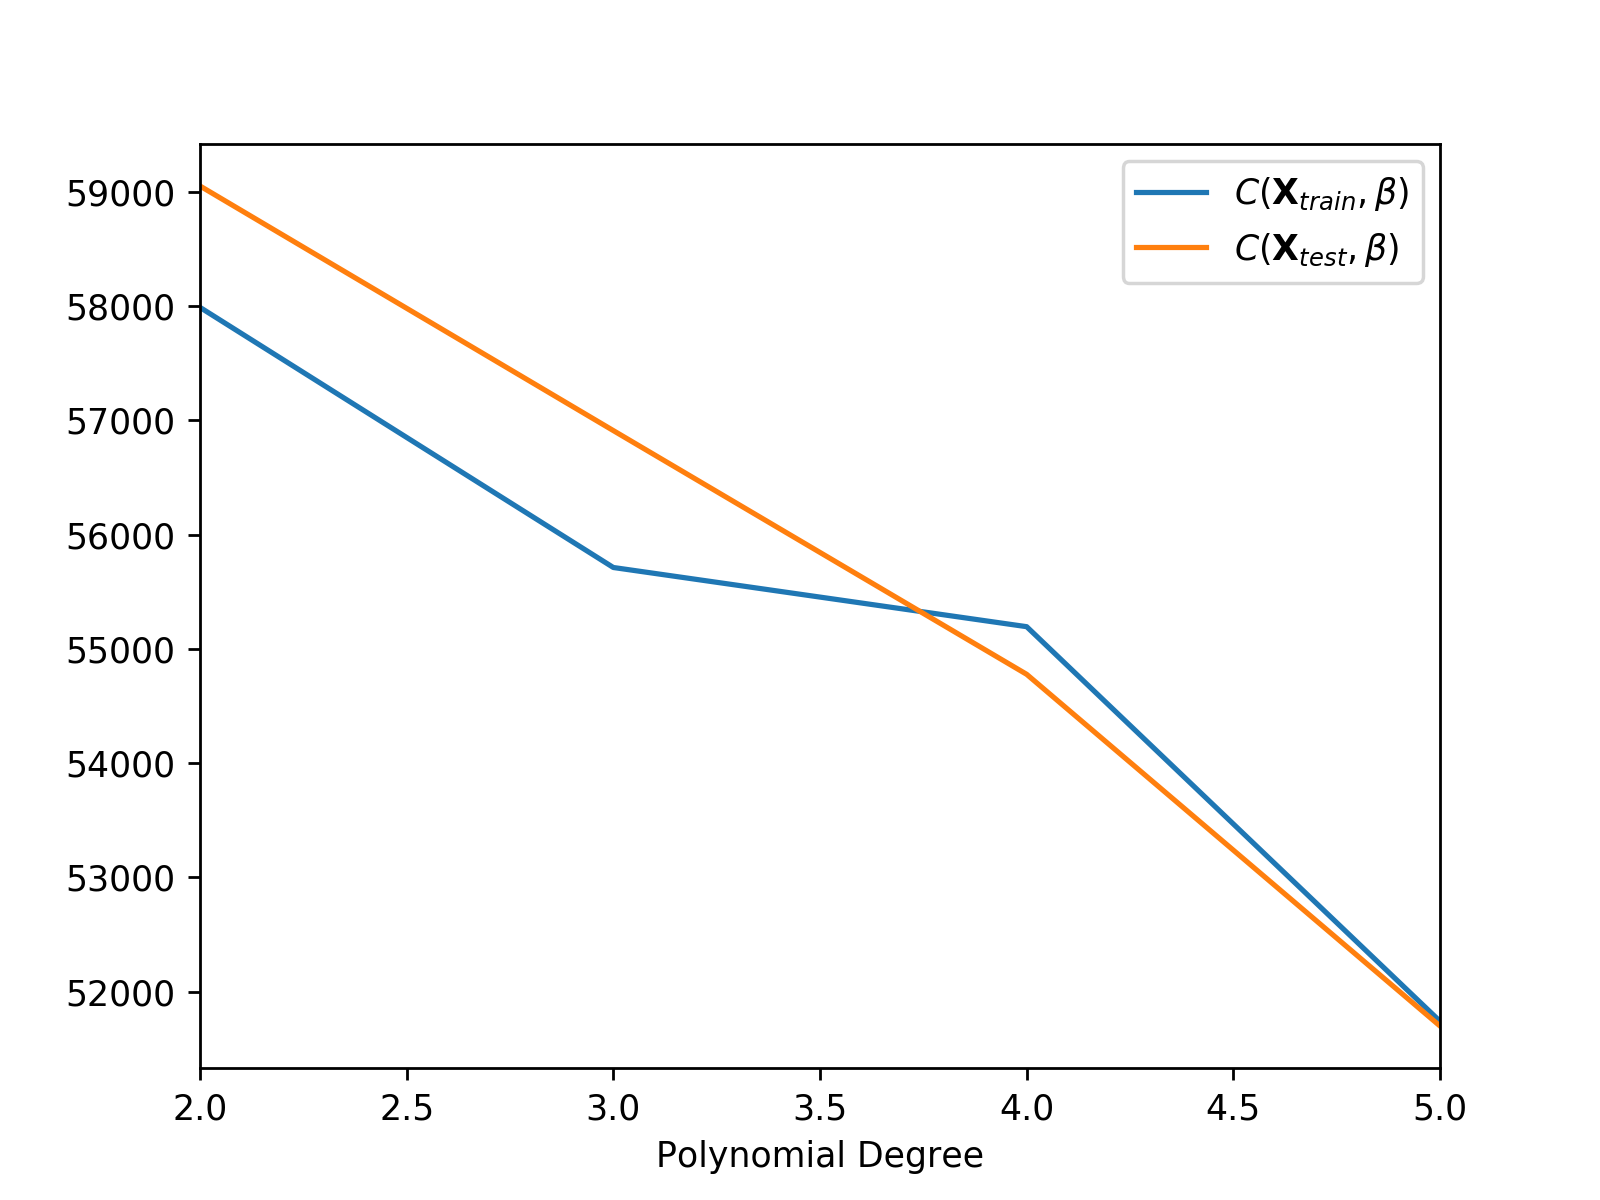
\includegraphics[width = 0.5\textwidth, center]{../real_output/part_C_2.png}
	\caption{The $MSE$ for the \textit{training data} and the \textit{testing data}, as a function of the polynomial degree after performing \textit{OLS} on real terrain data from \textit{Møsvatn Austfjell}}
	\label{part_g_c2}
\end{figure}

\begin{figure}[H]
	\centering 
	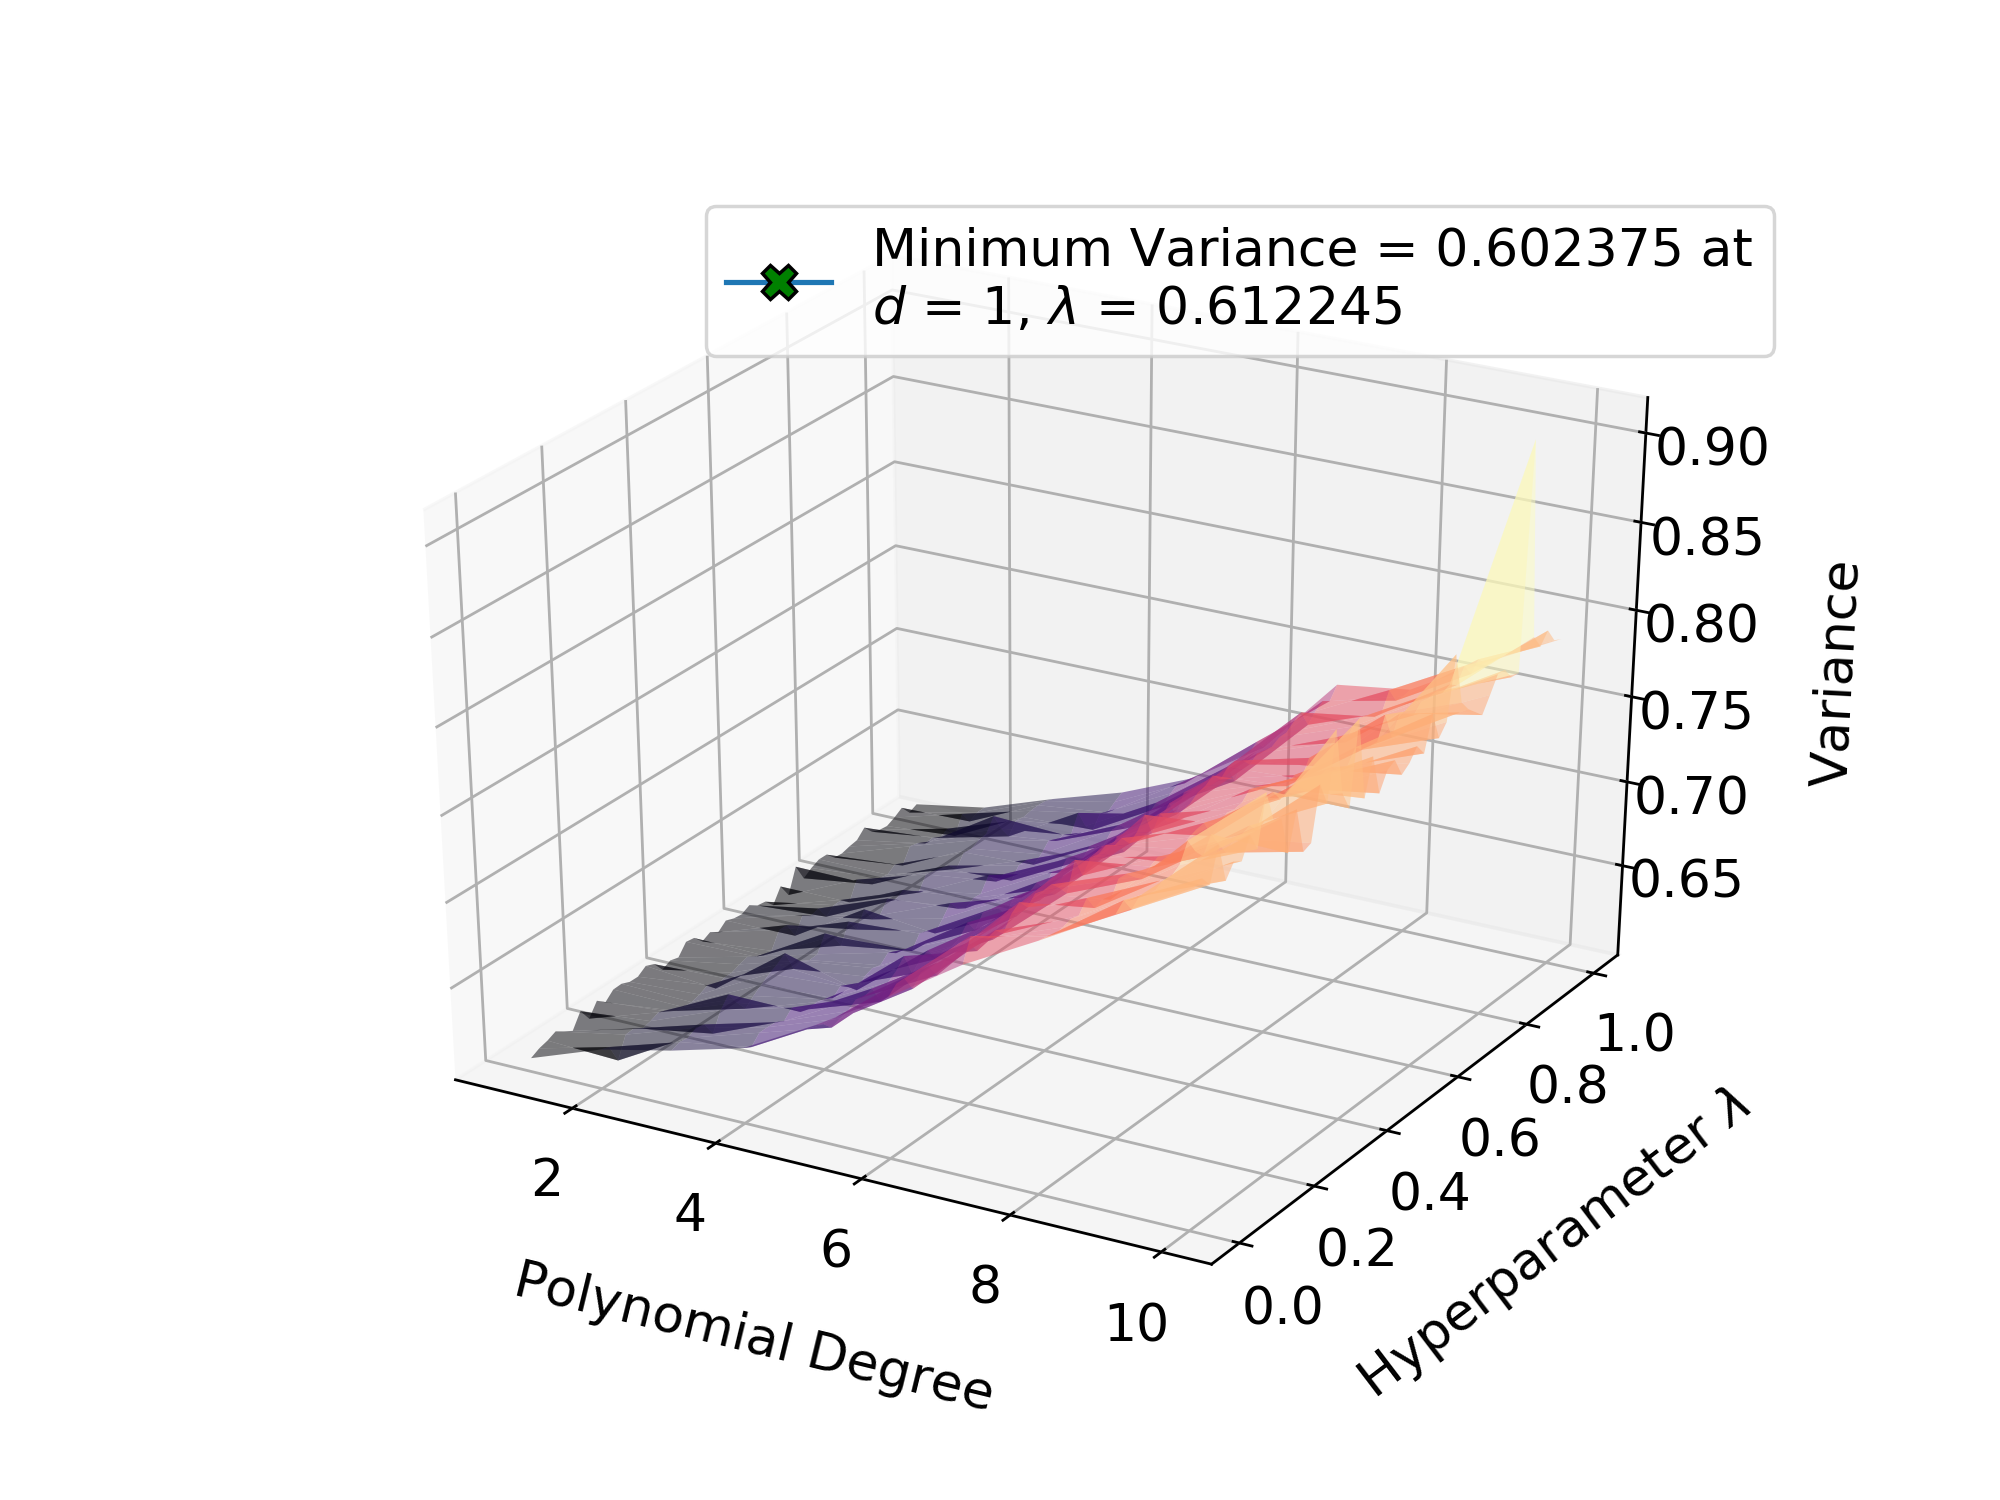
\includegraphics[width = 0.5\textwidth, center]{../real_output/part_D_1.png}
	\caption{The \textit{variance} as a function of the polynomial degree and hyperparameter $\lambda$ after performing \textit{Ridge regression} on real terrain data from \textit{Møsvatn Austfjell}}
	\label{part_g_d1}
\end{figure}

\begin{figure}[H]
	\centering 
	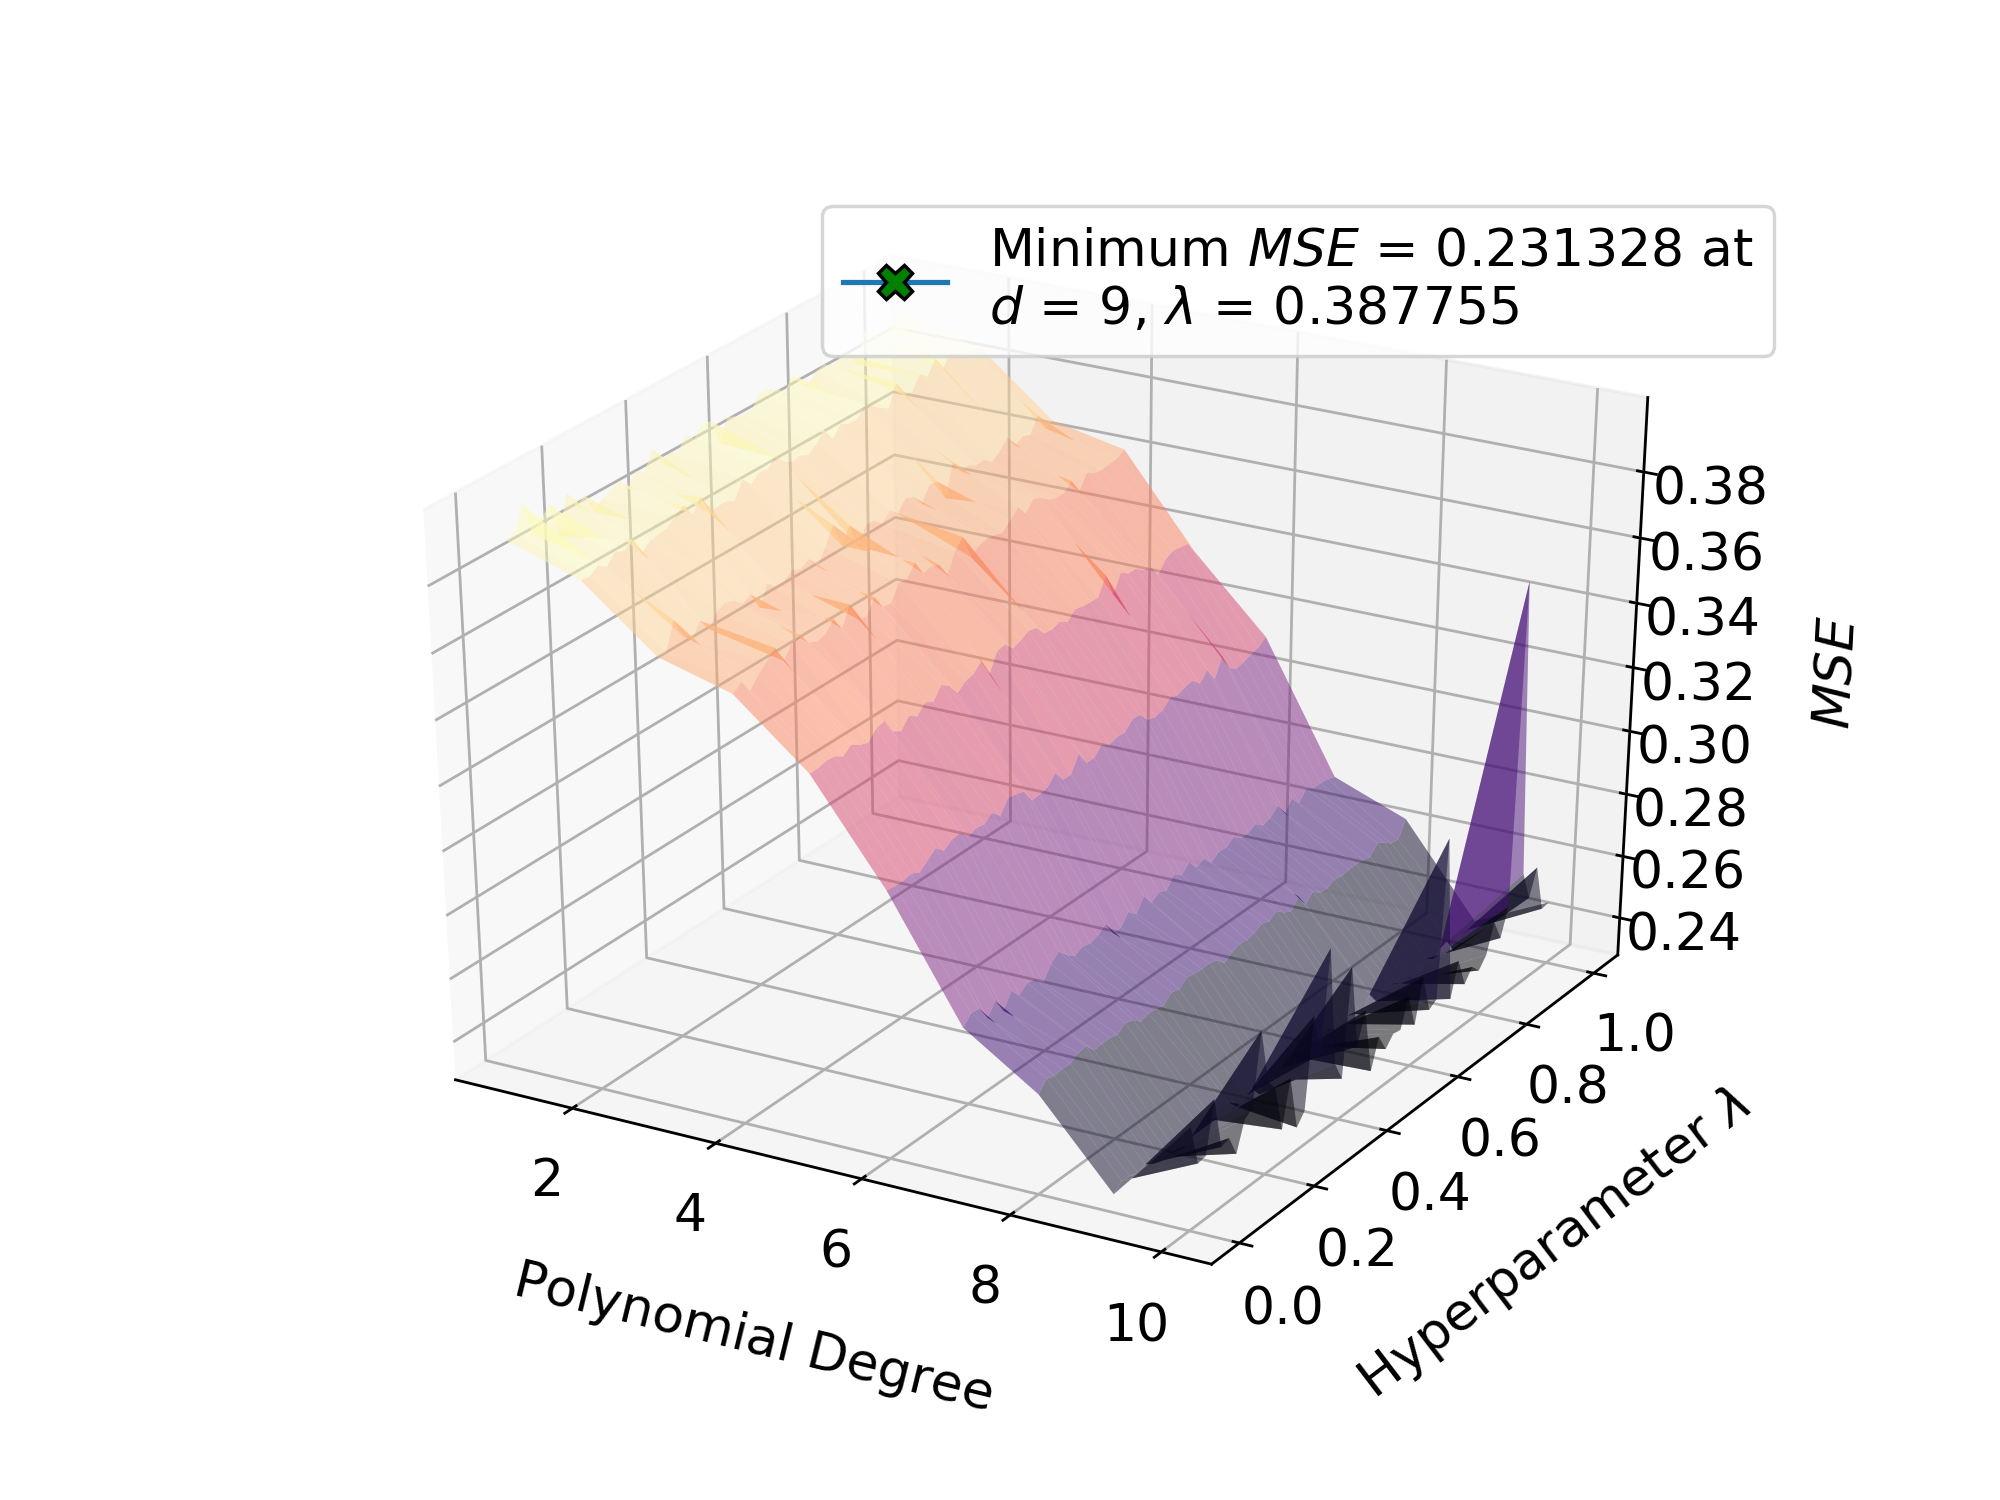
\includegraphics[width = 0.5\textwidth, center]{../real_output/part_D_2.png}
	\caption{The $MSE$ as a function of the polynomial degree and the hyperparameter $\lambda$ after performing \textit{Ridge regression} on real terrain data from \textit{Møsvatn Austfjell}}
	\label{part_g_d2}
\end{figure}

\begin{figure}[H]
	\centering 
	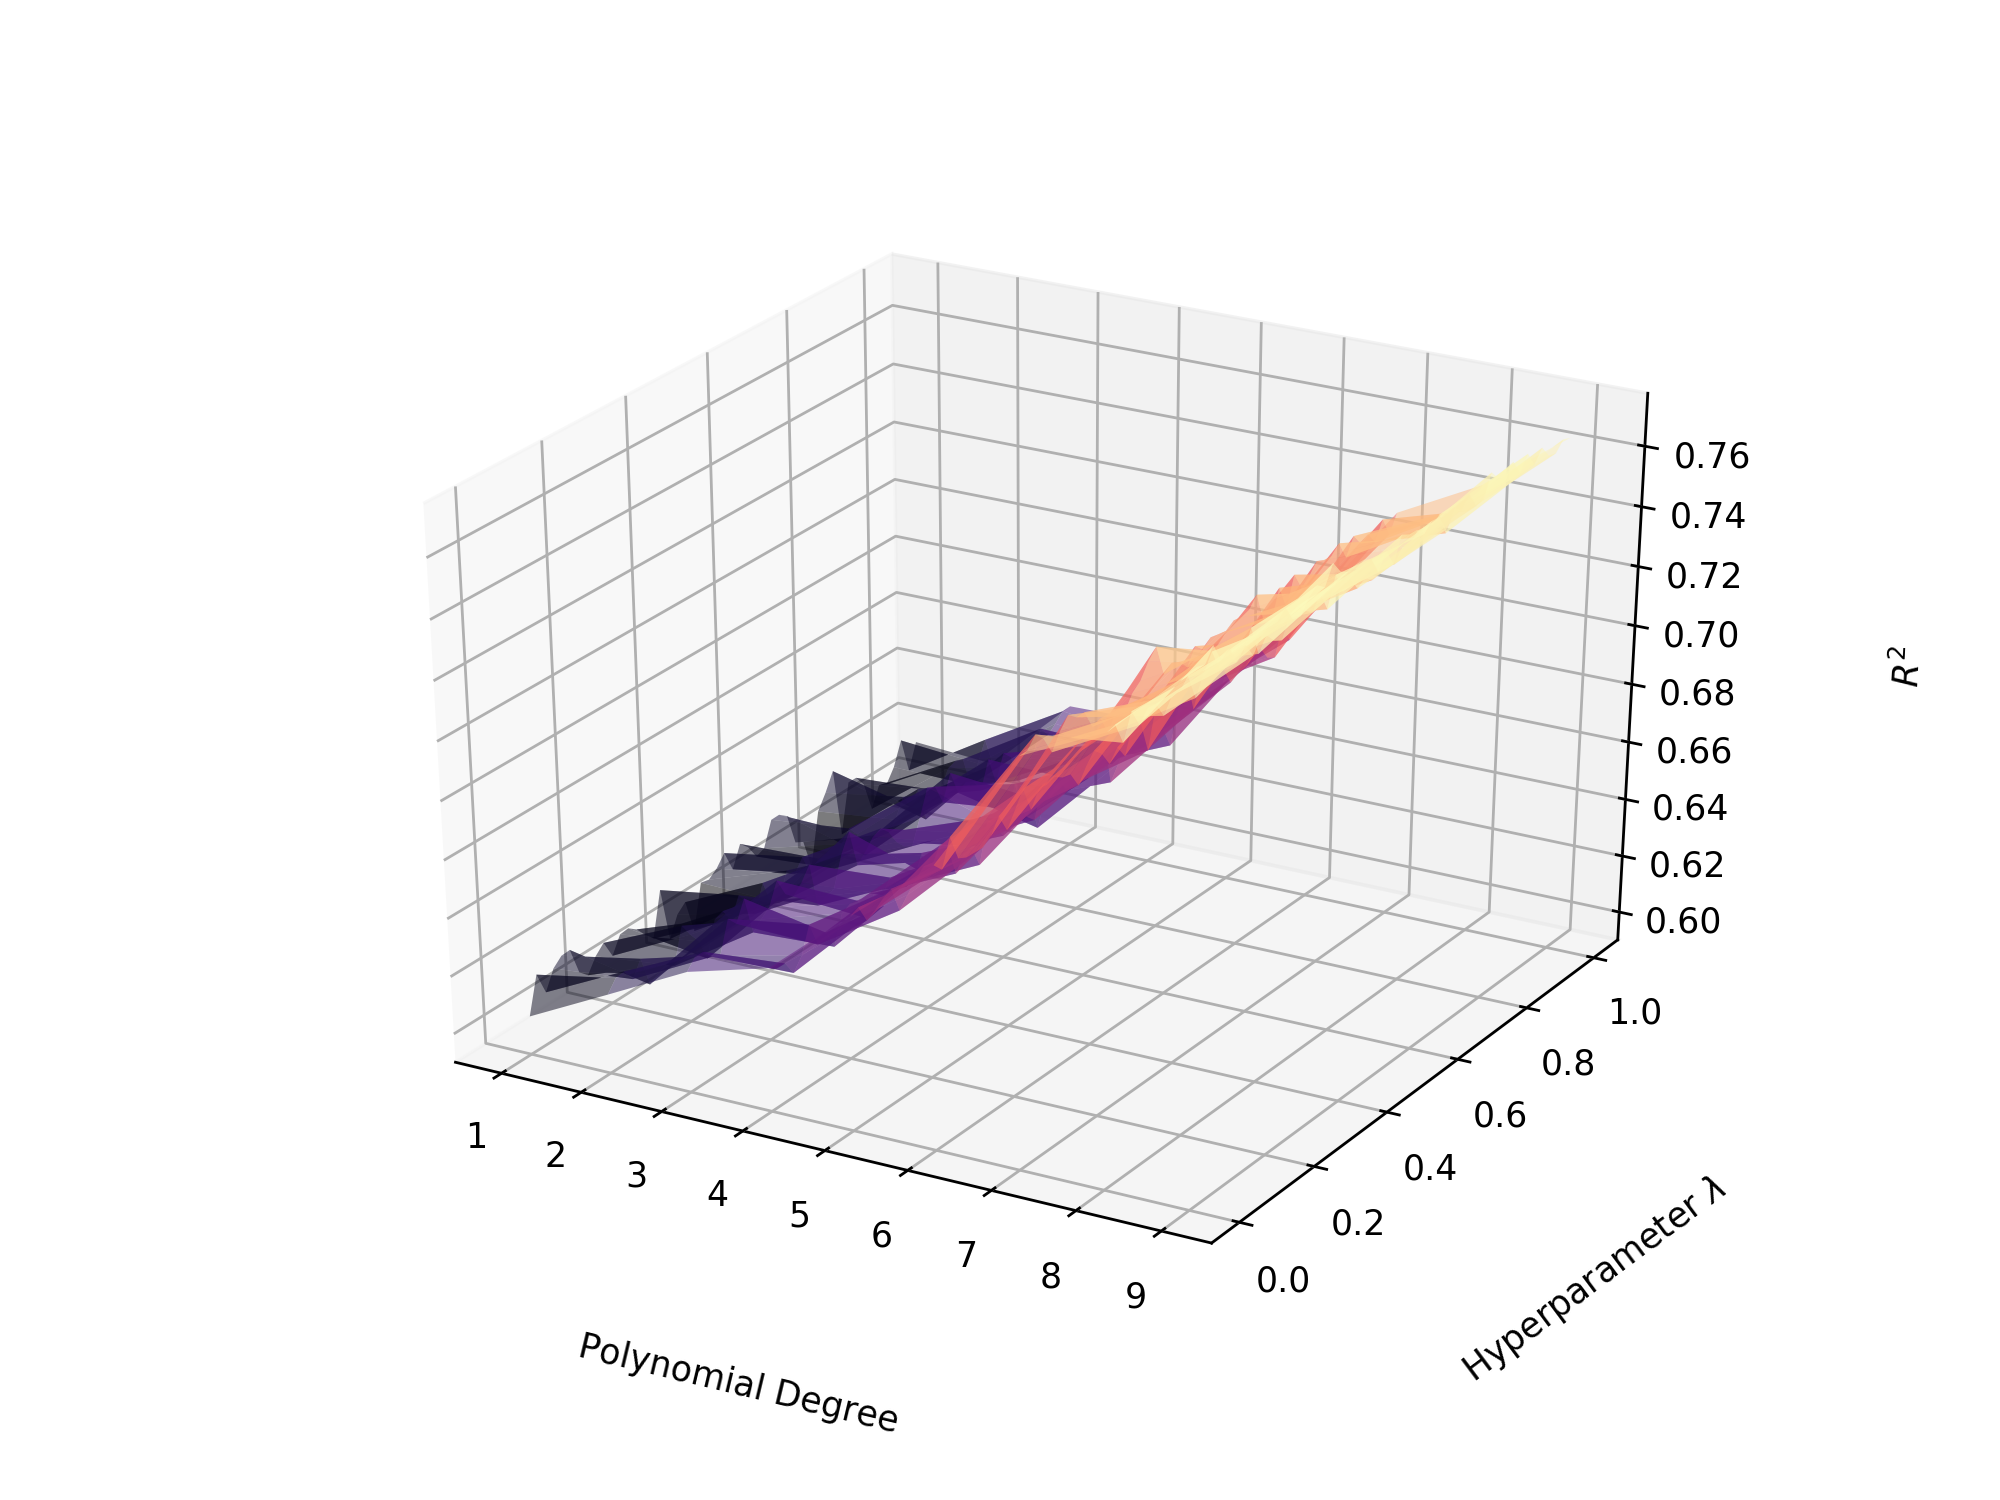
\includegraphics[width = 0.5\textwidth, center]{../real_output/part_D_3.png}
	\caption{The $R^2$-score as a function of the polynomial degree and hyperparameter $\lambda$ after performing \textit{Ridge regression} on real terrain data from \textit{Møsvatn Austfjell}}
	\label{part_g_d3}
\end{figure}

\begin{figure}[H]
	\centering 
	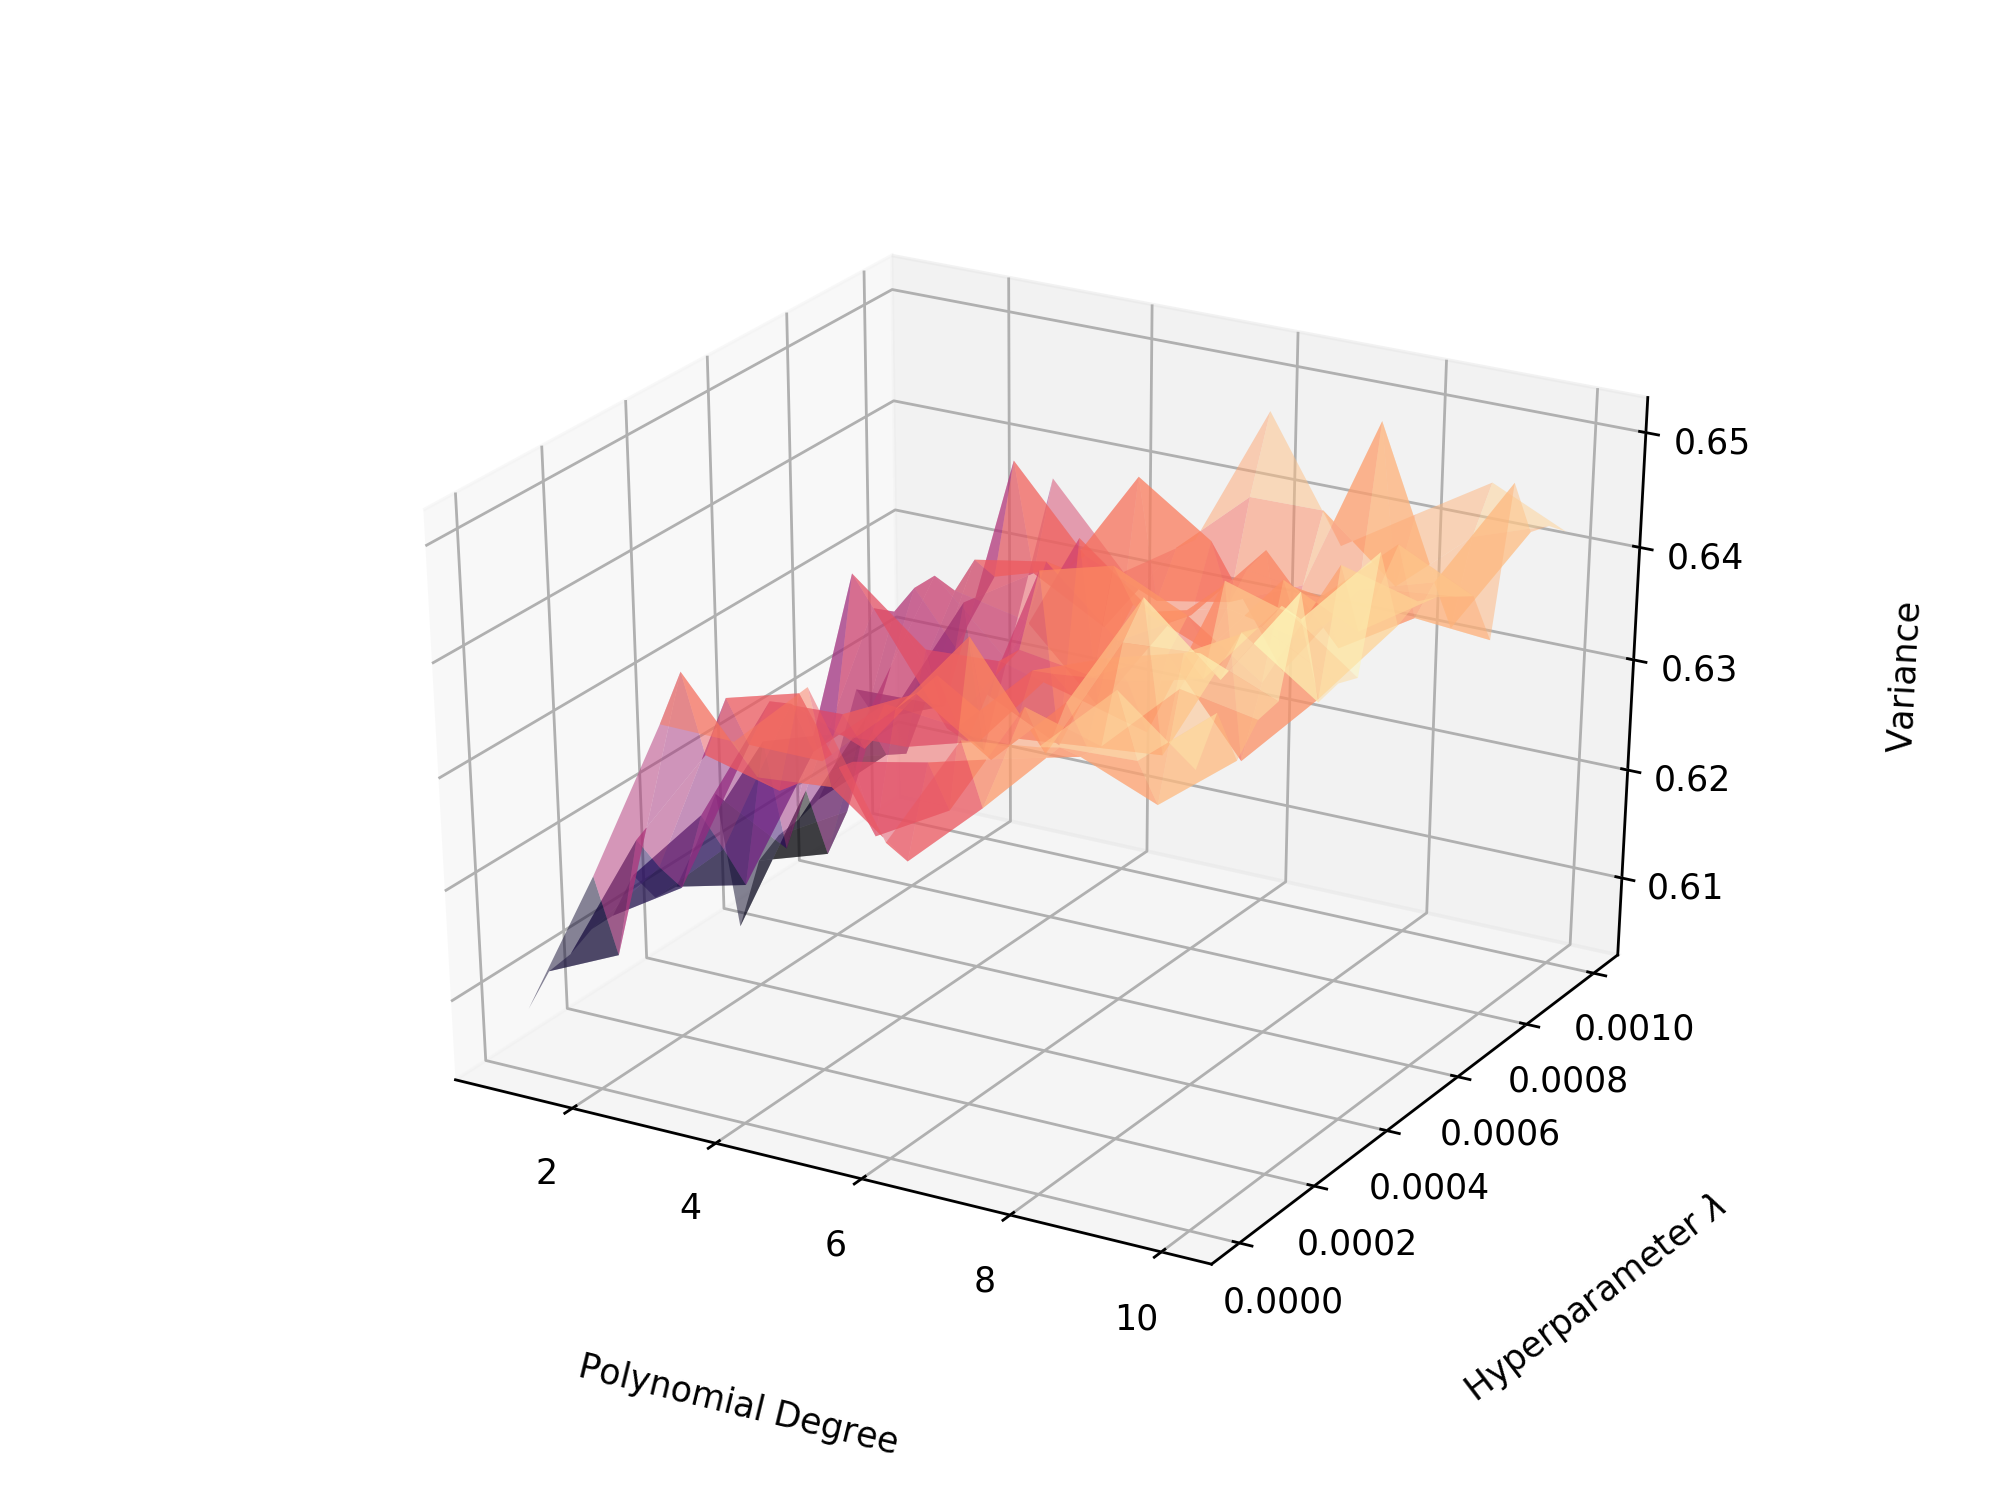
\includegraphics[width = 0.5\textwidth, center]{../real_output/part_E_1.png}
	\caption{The \textit{variance} as a function of the polynomial degree and hyperparameter $\lambda$ after performing \textit{LASSO regression} on real terrain data from \textit{Møsvatn Austfjell}}
	\label{part_g_e1}
\end{figure}

\begin{figure}[H]
	\centering 
	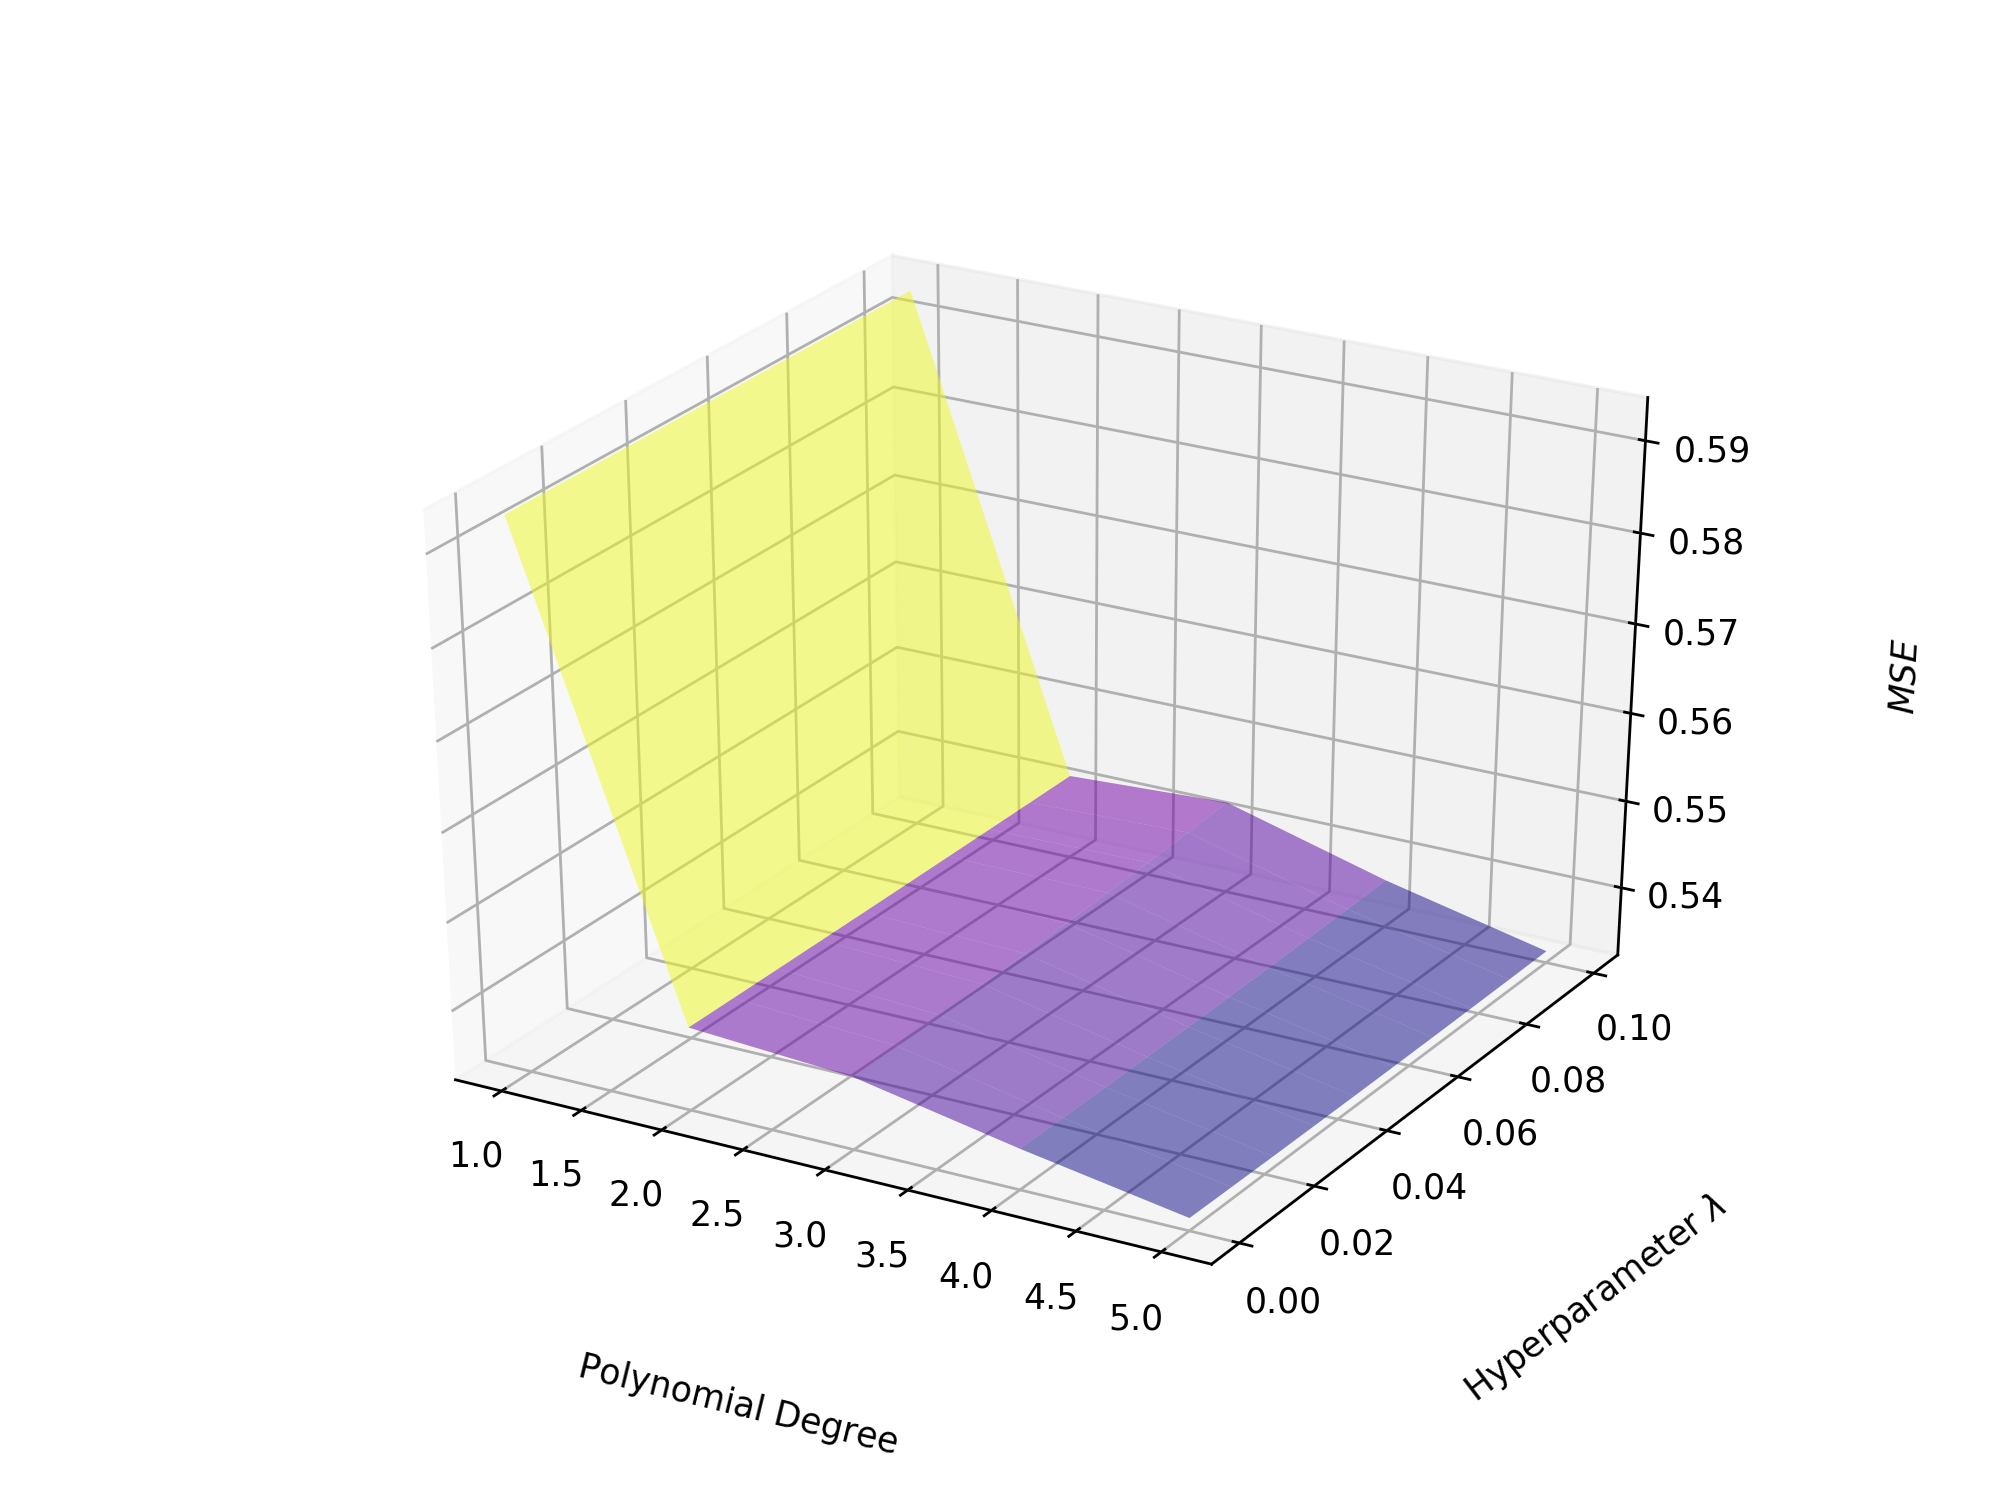
\includegraphics[width = 0.5\textwidth, center]{../real_output/part_E_2.png}
	\caption{Plots of the $MSE$ as a function of the polynomial degree and hyperparameter $\lambda$ after performing \textit{LASSO regression} on real terrain data from \textit{Møsvatn Austfjell}}
	\label{part_g_e2}
\end{figure}

\begin{figure}[H]
	\centering 
	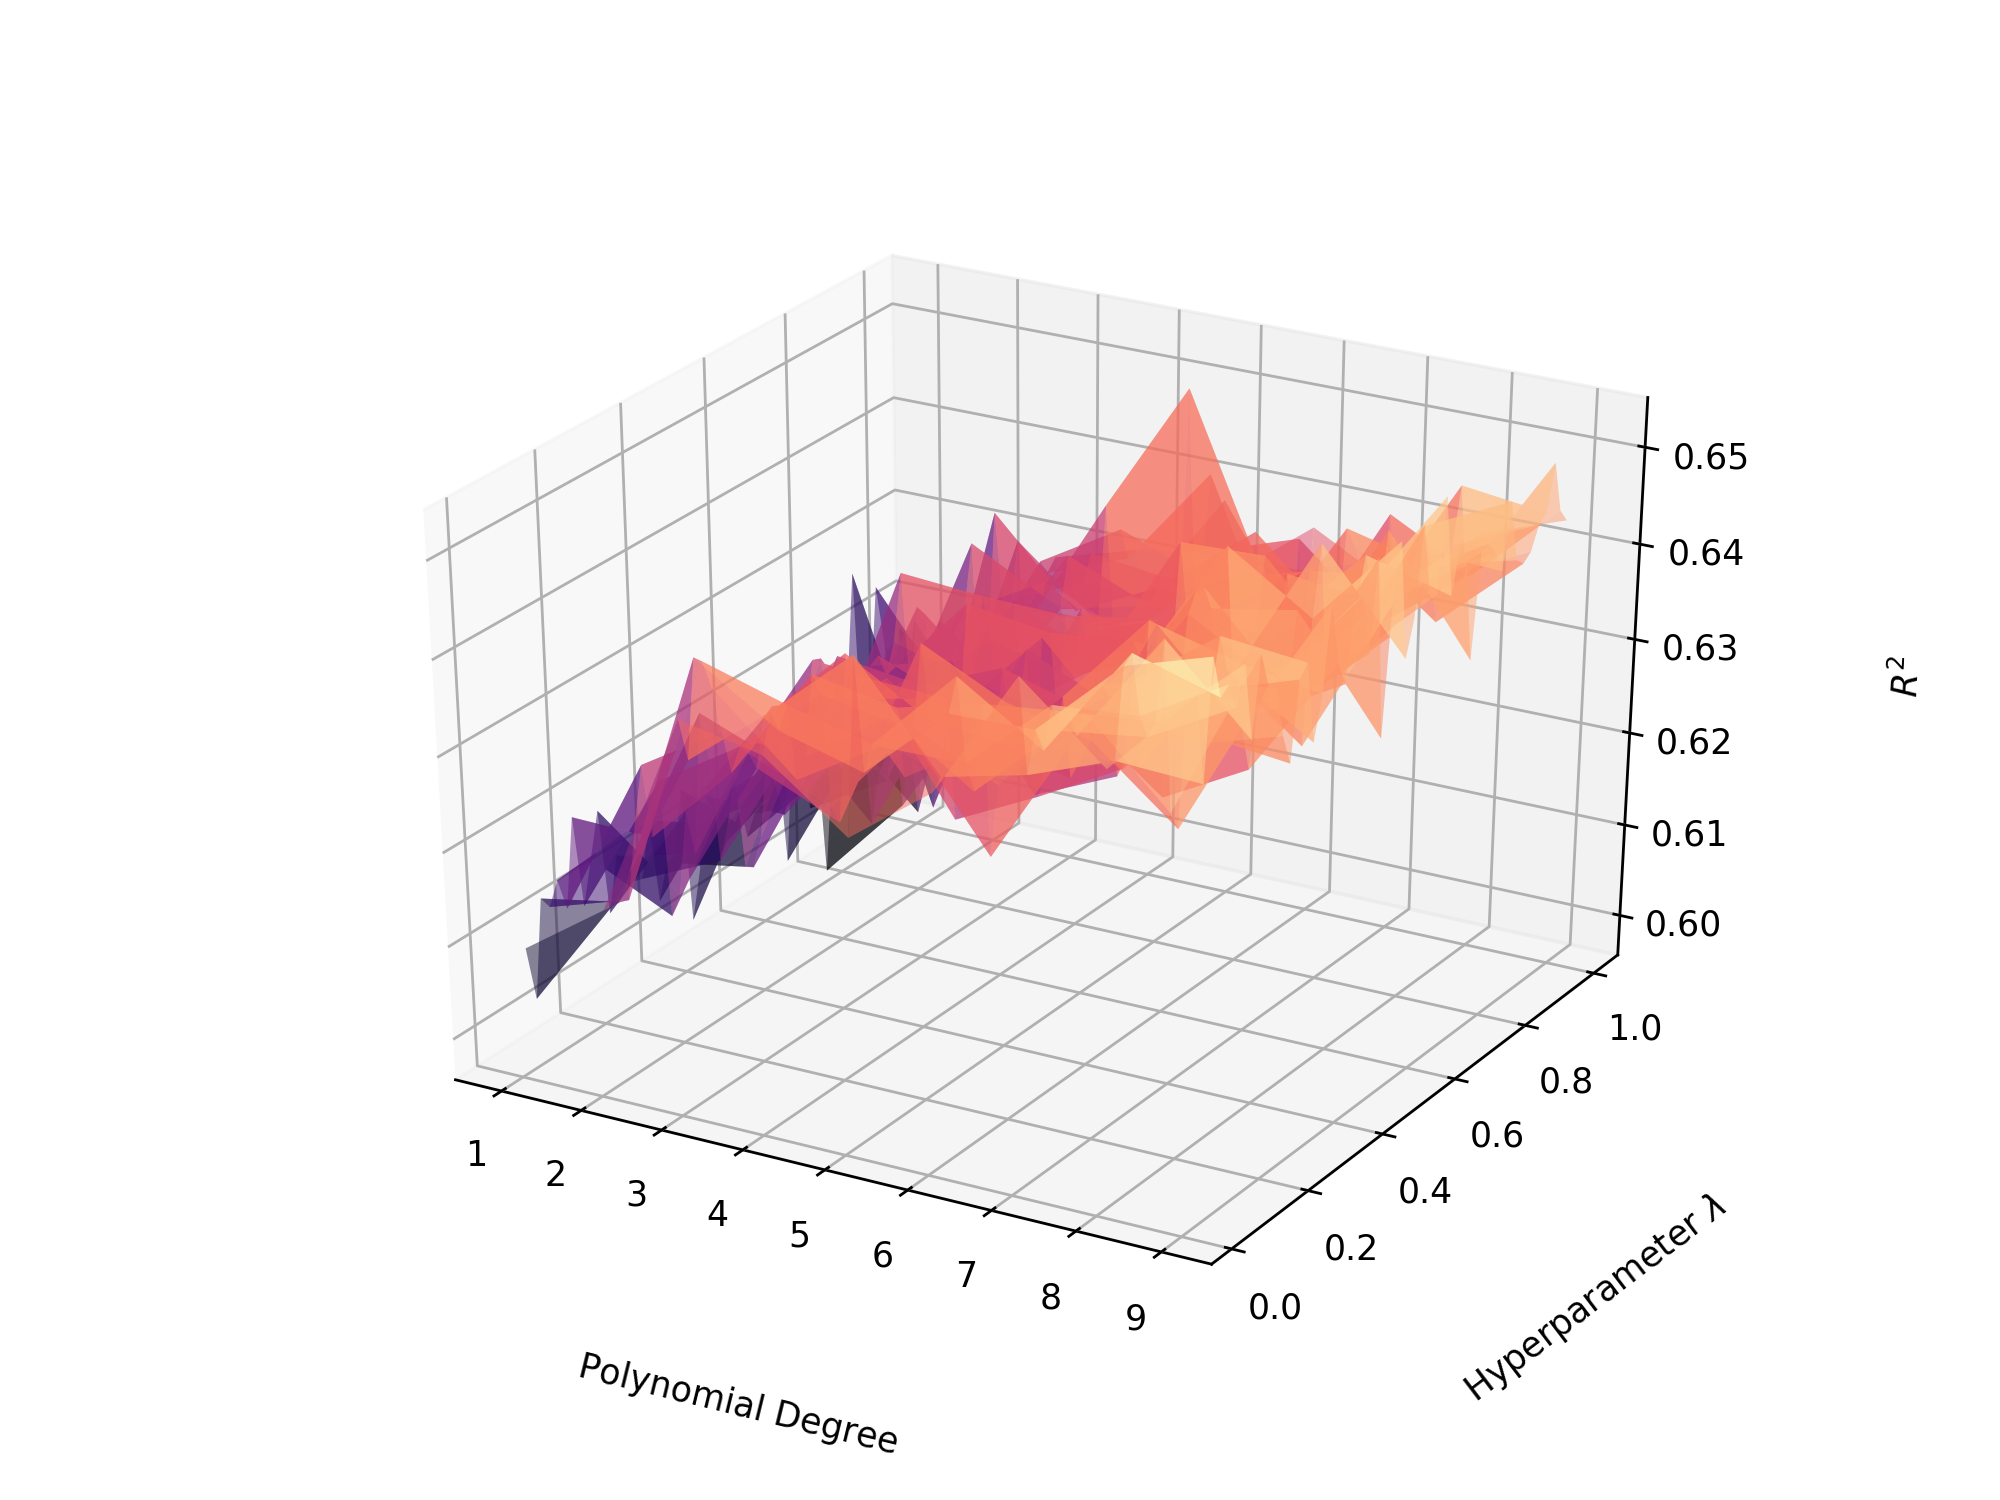
\includegraphics[width = 0.5\textwidth, center]{../real_output/part_E_3.png}
	\caption{The $R^2$-score as a function of the polynomial degre and hyperparameter $\lambda$ after performing \textit{LASSO regression} on real terrain data from \textit{Møsvatn Austfjell}}
	\label{part_g_e3}
\end{figure}




\section{Discussion}
\label{sec:discussion}

\subsection{franke}

Figure \ref{part_a}: varinace increases (bad?) as $n$ increases , but MSE$\rightarrow 0$ and $R^2\rightarrow 1$ (good). For $n=10$ we get overflow and weird results.

Figure \ref{part_b}: pretty similar results, no cross-validation give sligthly better reults, except at $n=9$, and cross-validation dosen't get overflow at $n=10$.

Figure \ref{part_c1}: not sure how to interpret this one. Also gives different results at $n=1$, which it shouldn't. Bias and variance differs, not quite sure what result is desirable.

Figure \ref{part_c2}: Pretty similar results for test and training, which I think is good, though train is slightly lower. Both have a minimum at $n=9$ and start increasing after that, as in figure \ref{part_b}. 

Figure \ref{part_d1}: Not moch to say here, the variance seems to flatten out as $n$ increases, suggesting diminishing returns. Much difference in result based on $\lambda$.

Figure \ref{part_d2}: Much the same as in figure \ref{part_d1}. Minimum MSE happens at $n=9$, which is before the overflow, suggesting that this is the highest $n$ can be before overflow. Minimum is also at lowest $\lambda$, suggesting that an even lower value could give even better results.

Figure \ref{part_d3}: Difference in results flattens out as $n$ increases. Not much difference in result based on $\lambda$, but best result happens at lower values, with a seeming spike at the lowest, coinsiding with the MSE. 

Figure \ref{part_d4}: Can't see any particular pattern here.

Figure \ref{part_e1}: Reults flattens out as $\lambda$ suggesting diminising results, but are highest for low $\lambda$. $n$ dosen't seem to have a large impact on variance.

Figure \ref{part_e2}: $n$ has a small impact on results. MSE drops quickly for lower $\lambda$. Best value at highest $n$ and lowest $\lambda$, suggesting a better result could be found for higher $n$ and lower $\lambda$.

Figure \ref{part_e3}: $n$ has a small impact on results. Best value at lower $\lambda$, coninciding with MSE. 

Figure \ref{part_e4}: Same as figure \ref{part_d4}.

OLS$>$Ridge$>$LASSO for MSE of Franke data. OLS and ridge best at $n=9$, LASSO at $n=10$. Best values at lowest $\lambda$ as well.


\subsubsection{real}

Figure \ref{part_g_a}: Pretty much what was expected, variance and MSE increases and $R^2$ decrases as $n$ increases. Total values are lower than for Franke, meaning higher uncertainty/data that is harder to interpret/fit to polynomial, makes sense as it's real life data. More or less exact overlap between variance and $R^2$.

Figure \ref{part_g_b}: Results are slightly better than without cross-validation.

Figure \ref{part_g_c2}: MSE of train and test is pretty close, though more variance in test.

Figure \ref{part_g_d1}: Unlike Franke, the data dosen't flatten out for any particular variable

Figure \ref{part_g_d2}: Best result not at a extreme for $\lambda$, suggesting either that the best result is within tested $\lambda$-values or relativley low impact from $\lambda$. Best result is at highest tested $n$, but there's unlikely to be a beter result as $n=10$ gave overflow. Minimum MSE is smaller than for Franke, as figure \ref{part_g_a}. 

Figure \ref{part_g_d3}: Same as figure \ref{part_g_d1}.

Figure \ref{part_g_e1}: More spikes/variance than Ridge. 

Figure \ref{part_g_e2}: Best MSE is neither for lowest $\lambda$ or highest $n$.

Figure \ref{part_g_e3}: 


Ridge$>$OLS$>$LASSO for real data. OLS and Ridge at $n=9$ and LASSO at $n=8$.


we should maybe have a plot of made from the betas at the smalest MSE

\newpage

\section{Appendix}
\label{sec:appendix}

\bibliography{bib}{}
\bibliographystyle{ieeetr}


\end{document}


















